\documentclass[]{book}
\usepackage{lmodern}
\usepackage{amssymb,amsmath}
\usepackage{ifxetex,ifluatex}
\usepackage{fixltx2e} % provides \textsubscript
\ifnum 0\ifxetex 1\fi\ifluatex 1\fi=0 % if pdftex
  \usepackage[T1]{fontenc}
  \usepackage[utf8]{inputenc}
\else % if luatex or xelatex
  \ifxetex
    \usepackage{mathspec}
  \else
    \usepackage{fontspec}
  \fi
  \defaultfontfeatures{Ligatures=TeX,Scale=MatchLowercase}
  \newcommand{\euro}{€}
\fi
% use upquote if available, for straight quotes in verbatim environments
\IfFileExists{upquote.sty}{\usepackage{upquote}}{}
% use microtype if available
\IfFileExists{microtype.sty}{%
\usepackage{microtype}
\UseMicrotypeSet[protrusion]{basicmath} % disable protrusion for tt fonts
}{}
\usepackage[margin=1in]{geometry}
\usepackage{hyperref}
\PassOptionsToPackage{usenames,dvipsnames}{color} % color is loaded by hyperref
\hypersetup{unicode=true,
            pdftitle={Solutions to Time Series Analysis: with Applications in R},
            pdfauthor={Johan Larsson},
            pdfborder={0 0 0},
            breaklinks=true}
\urlstyle{same}  % don't use monospace font for urls
\usepackage{color}
\usepackage{fancyvrb}
\newcommand{\VerbBar}{|}
\newcommand{\VERB}{\Verb[commandchars=\\\{\}]}
\DefineVerbatimEnvironment{Highlighting}{Verbatim}{commandchars=\\\{\}}
% Add ',fontsize=\small' for more characters per line
\usepackage{framed}
\definecolor{shadecolor}{RGB}{248,248,248}
\newenvironment{Shaded}{\begin{snugshade}}{\end{snugshade}}
\newcommand{\KeywordTok}[1]{\textcolor[rgb]{0.13,0.29,0.53}{\textbf{{#1}}}}
\newcommand{\DataTypeTok}[1]{\textcolor[rgb]{0.13,0.29,0.53}{{#1}}}
\newcommand{\DecValTok}[1]{\textcolor[rgb]{0.00,0.00,0.81}{{#1}}}
\newcommand{\BaseNTok}[1]{\textcolor[rgb]{0.00,0.00,0.81}{{#1}}}
\newcommand{\FloatTok}[1]{\textcolor[rgb]{0.00,0.00,0.81}{{#1}}}
\newcommand{\ConstantTok}[1]{\textcolor[rgb]{0.00,0.00,0.00}{{#1}}}
\newcommand{\CharTok}[1]{\textcolor[rgb]{0.31,0.60,0.02}{{#1}}}
\newcommand{\SpecialCharTok}[1]{\textcolor[rgb]{0.00,0.00,0.00}{{#1}}}
\newcommand{\StringTok}[1]{\textcolor[rgb]{0.31,0.60,0.02}{{#1}}}
\newcommand{\VerbatimStringTok}[1]{\textcolor[rgb]{0.31,0.60,0.02}{{#1}}}
\newcommand{\SpecialStringTok}[1]{\textcolor[rgb]{0.31,0.60,0.02}{{#1}}}
\newcommand{\ImportTok}[1]{{#1}}
\newcommand{\CommentTok}[1]{\textcolor[rgb]{0.56,0.35,0.01}{\textit{{#1}}}}
\newcommand{\DocumentationTok}[1]{\textcolor[rgb]{0.56,0.35,0.01}{\textbf{\textit{{#1}}}}}
\newcommand{\AnnotationTok}[1]{\textcolor[rgb]{0.56,0.35,0.01}{\textbf{\textit{{#1}}}}}
\newcommand{\CommentVarTok}[1]{\textcolor[rgb]{0.56,0.35,0.01}{\textbf{\textit{{#1}}}}}
\newcommand{\OtherTok}[1]{\textcolor[rgb]{0.56,0.35,0.01}{{#1}}}
\newcommand{\FunctionTok}[1]{\textcolor[rgb]{0.00,0.00,0.00}{{#1}}}
\newcommand{\VariableTok}[1]{\textcolor[rgb]{0.00,0.00,0.00}{{#1}}}
\newcommand{\ControlFlowTok}[1]{\textcolor[rgb]{0.13,0.29,0.53}{\textbf{{#1}}}}
\newcommand{\OperatorTok}[1]{\textcolor[rgb]{0.81,0.36,0.00}{\textbf{{#1}}}}
\newcommand{\BuiltInTok}[1]{{#1}}
\newcommand{\ExtensionTok}[1]{{#1}}
\newcommand{\PreprocessorTok}[1]{\textcolor[rgb]{0.56,0.35,0.01}{\textit{{#1}}}}
\newcommand{\AttributeTok}[1]{\textcolor[rgb]{0.77,0.63,0.00}{{#1}}}
\newcommand{\RegionMarkerTok}[1]{{#1}}
\newcommand{\InformationTok}[1]{\textcolor[rgb]{0.56,0.35,0.01}{\textbf{\textit{{#1}}}}}
\newcommand{\WarningTok}[1]{\textcolor[rgb]{0.56,0.35,0.01}{\textbf{\textit{{#1}}}}}
\newcommand{\AlertTok}[1]{\textcolor[rgb]{0.94,0.16,0.16}{{#1}}}
\newcommand{\ErrorTok}[1]{\textcolor[rgb]{0.64,0.00,0.00}{\textbf{{#1}}}}
\newcommand{\NormalTok}[1]{{#1}}
\usepackage{longtable,booktabs}
\usepackage{graphicx,grffile}
\makeatletter
\def\maxwidth{\ifdim\Gin@nat@width>\linewidth\linewidth\else\Gin@nat@width\fi}
\def\maxheight{\ifdim\Gin@nat@height>\textheight\textheight\else\Gin@nat@height\fi}
\makeatother
% Scale images if necessary, so that they will not overflow the page
% margins by default, and it is still possible to overwrite the defaults
% using explicit options in \includegraphics[width, height, ...]{}
\setkeys{Gin}{width=\maxwidth,height=\maxheight,keepaspectratio}
\setlength{\parindent}{0pt}
\setlength{\parskip}{6pt plus 2pt minus 1pt}
\setlength{\emergencystretch}{3em}  % prevent overfull lines
\providecommand{\tightlist}{%
  \setlength{\itemsep}{0pt}\setlength{\parskip}{0pt}}
\setcounter{secnumdepth}{5}

%%% Use protect on footnotes to avoid problems with footnotes in titles
\let\rmarkdownfootnote\footnote%
\def\footnote{\protect\rmarkdownfootnote}

%%% Change title format to be more compact
\usepackage{titling}

% Create subtitle command for use in maketitle
\newcommand{\subtitle}[1]{
  \posttitle{
    \begin{center}\large#1\end{center}
    }
}

\setlength{\droptitle}{-2em}
  \title{Solutions to Time Series Analysis: with Applications in R}
  \pretitle{\vspace{\droptitle}\centering\huge}
  \posttitle{\par}
  \author{Johan Larsson}
  \preauthor{\centering\large\emph}
  \postauthor{\par}
  \predate{\centering\large\emph}
  \postdate{\par}
  \date{2017-04-05}


% Redefines (sub)paragraphs to behave more like sections
\ifx\paragraph\undefined\else
\let\oldparagraph\paragraph
\renewcommand{\paragraph}[1]{\oldparagraph{#1}\mbox{}}
\fi
\ifx\subparagraph\undefined\else
\let\oldsubparagraph\subparagraph
\renewcommand{\subparagraph}[1]{\oldsubparagraph{#1}\mbox{}}
\fi


\usepackage{amsthm}
\newtheorem{theorem}{Theorem}[chapter]
\newtheorem{lemma}{Lemma}[chapter]
\theoremstyle{definition}
\newtheorem{definition}{Definition}[chapter]
\newtheorem{corollary}{Corollary}[chapter]
\newtheorem{proposition}{Proposition}[chapter]
\theoremstyle{definition}
\newtheorem{example}{Example}[chapter]
\theoremstyle{remark}
\newtheorem*{remark}{Remark}
\begin{document}
\maketitle

{
\setcounter{tocdepth}{1}
\tableofcontents
}
\chapter*{Preface}\label{preface}
\addcontentsline{toc}{chapter}{Preface}

This book contains solutions to the problems in the book \emph{Time
Series Analysis: with Applications in R}, third edition, by Cryer and
Chan. It is provided as a github repository so that anybody may
contribute to its development.

\section*{Dependencies}\label{dependencies}
\addcontentsline{toc}{section}{Dependencies}

You will need these packages to reproduce the examples in this book:

\begin{Shaded}
\begin{Highlighting}[]
\KeywordTok{install.packages}\NormalTok{(}\KeywordTok{c}\NormalTok{(}
  \StringTok{"latticeExtra"}\NormalTok{,}
  \StringTok{"lattice"}\NormalTok{,}
  \StringTok{"TSA"}\NormalTok{,}
  \StringTok{"pander"}
\NormalTok{))}
\end{Highlighting}
\end{Shaded}

\begin{Shaded}
\begin{Highlighting}[]
\CommentTok{# Load the packages}
\KeywordTok{library}\NormalTok{(latticeExtra)}
\KeywordTok{library}\NormalTok{(TSA)}
\KeywordTok{library}\NormalTok{(pander)}
\KeywordTok{library}\NormalTok{(dplyr)}
\end{Highlighting}
\end{Shaded}

In order for some of the content in this book to be reproducible, the
random seed is set as follows.

\begin{Shaded}
\begin{Highlighting}[]
\KeywordTok{set.seed}\NormalTok{(}\DecValTok{1234}\NormalTok{)}
\end{Highlighting}
\end{Shaded}

\chapter{Introduction}\label{introduction}

\section{Larain}\label{larain}

\begin{quote}
Use software to produce the time series plot shown in Exhibit 1.2, on
page 2. The data are in the file named larain.
\end{quote}

\begin{Shaded}
\begin{Highlighting}[]
\KeywordTok{library}\NormalTok{(TSA)}
\KeywordTok{library}\NormalTok{(latticeExtra)}

\KeywordTok{data}\NormalTok{(larain, }\DataTypeTok{package =} \StringTok{"TSA"}\NormalTok{)}
\end{Highlighting}
\end{Shaded}

\begin{Shaded}
\begin{Highlighting}[]
\KeywordTok{xyplot}\NormalTok{(larain, }\DataTypeTok{ylab =} \StringTok{"Inches"}\NormalTok{, }\DataTypeTok{xlab =} \StringTok{"Year"}\NormalTok{, }\DataTypeTok{type =} \StringTok{"o"}\NormalTok{)}
\end{Highlighting}
\end{Shaded}

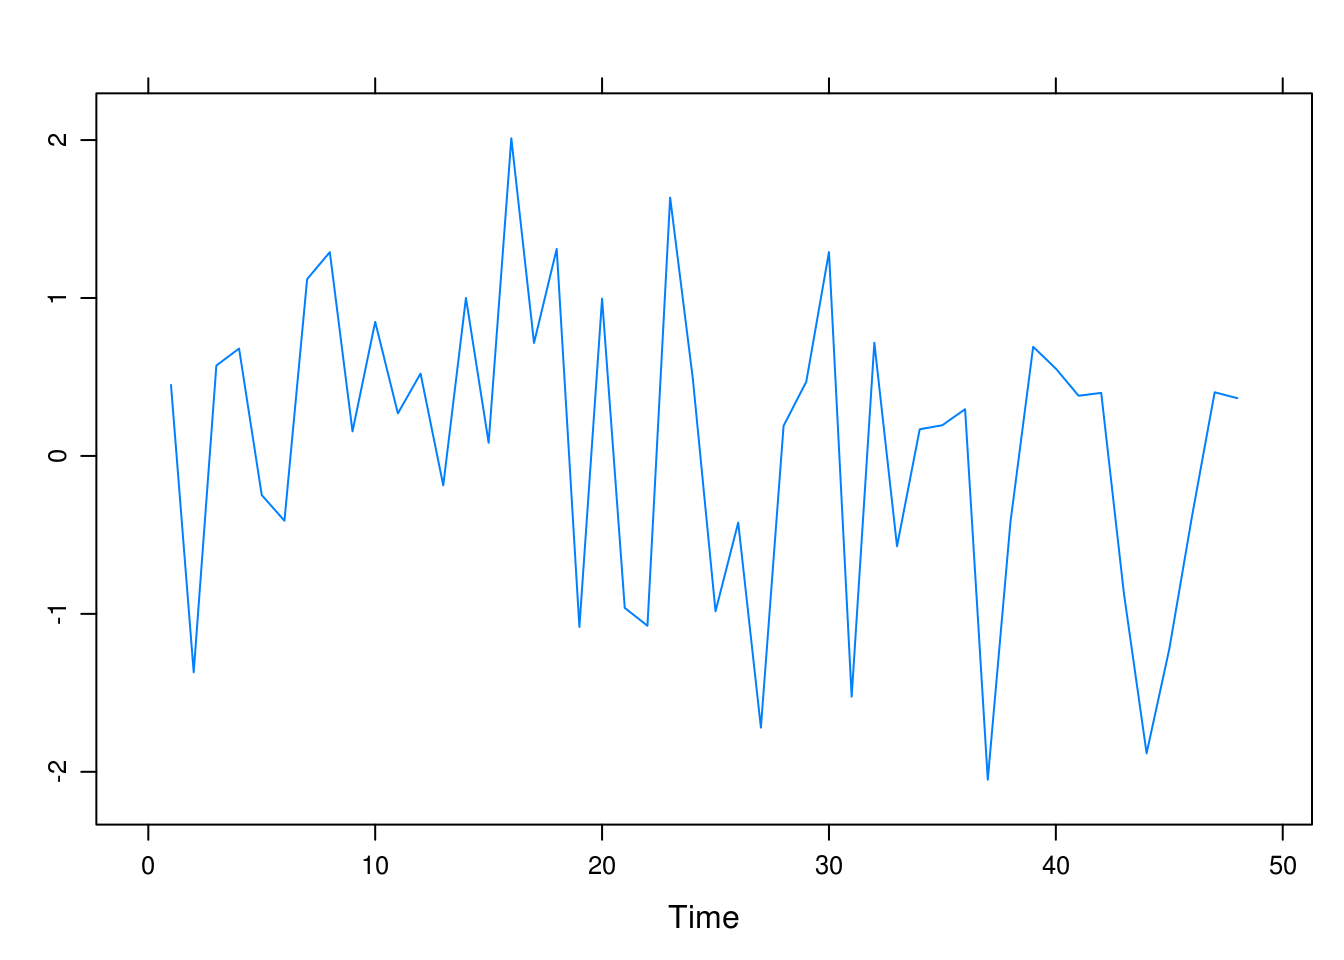
\includegraphics{TSAsolutions_files/figure-latex/unnamed-chunk-3-1.pdf}

\section{Colors}\label{colors}

\begin{quote}
Produce the time series plot displayed in Exhibit 1.3, on page 3. The
data file is named color.
\end{quote}

\begin{Shaded}
\begin{Highlighting}[]
\KeywordTok{data}\NormalTok{(color)}
\KeywordTok{xyplot}\NormalTok{(color, }\DataTypeTok{ylab =} \StringTok{"Color property"}\NormalTok{, }\DataTypeTok{xlab =} \StringTok{"Batch"}\NormalTok{, }\DataTypeTok{type =} \StringTok{"o"}\NormalTok{)}
\end{Highlighting}
\end{Shaded}

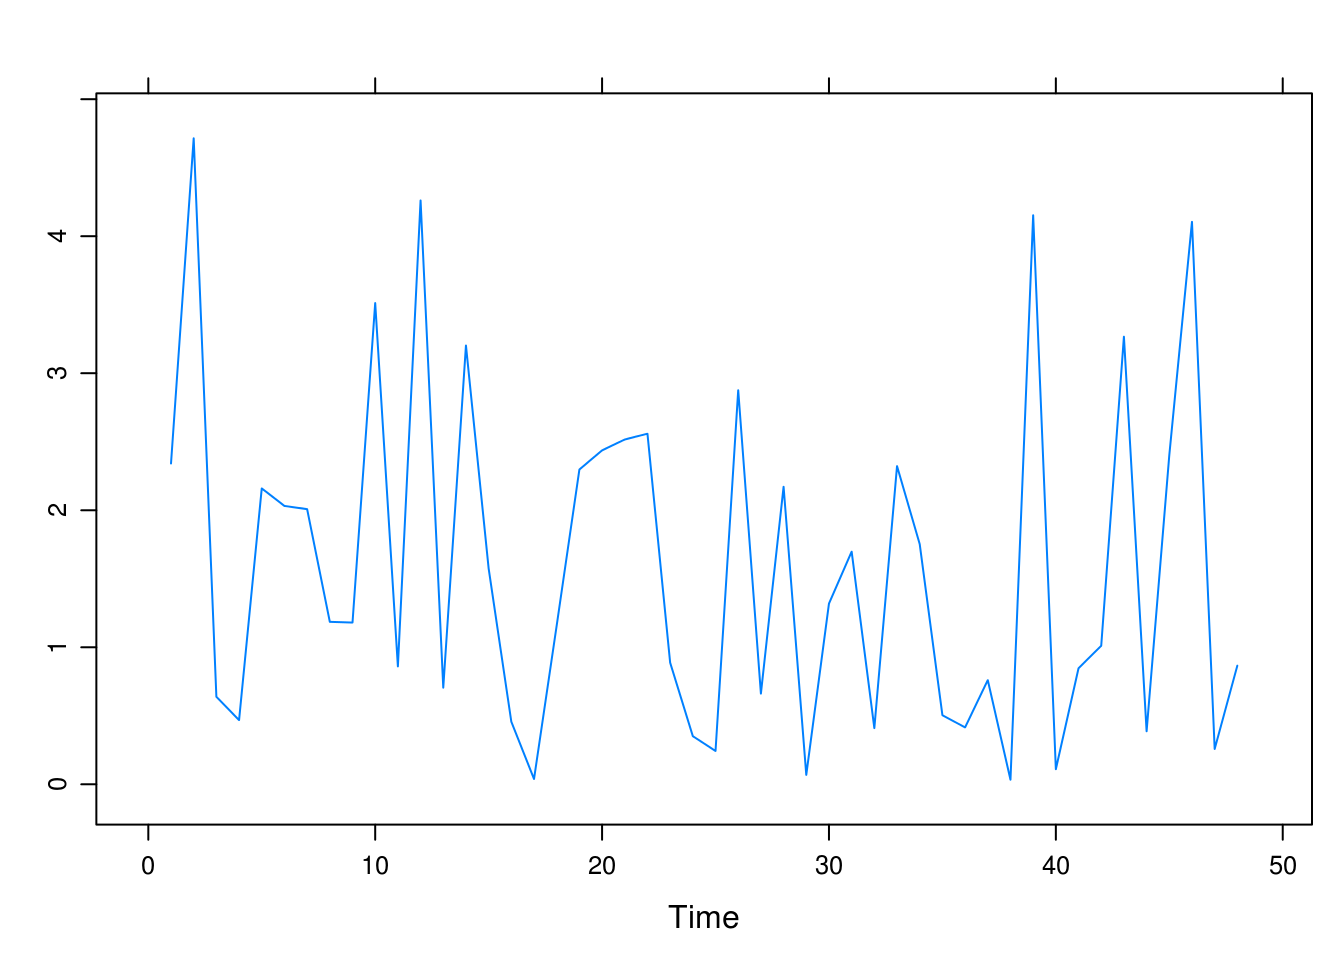
\includegraphics{TSAsolutions_files/figure-latex/unnamed-chunk-4-1.pdf}

\section{Random, normal time series}\label{random-normal-time-series}

\begin{quote}
Simulate a completely random process of length 48 with independent,
normal values. Plot the time series plot. Does it look ``random''?
Repeat this exercise several times with a new simulation each time.
\end{quote}

\begin{Shaded}
\begin{Highlighting}[]
\KeywordTok{xyplot}\NormalTok{(}\KeywordTok{as.ts}\NormalTok{(}\KeywordTok{rnorm}\NormalTok{(}\DecValTok{48}\NormalTok{)))}
\KeywordTok{xyplot}\NormalTok{(}\KeywordTok{as.ts}\NormalTok{(}\KeywordTok{rnorm}\NormalTok{(}\DecValTok{48}\NormalTok{)))}
\end{Highlighting}
\end{Shaded}

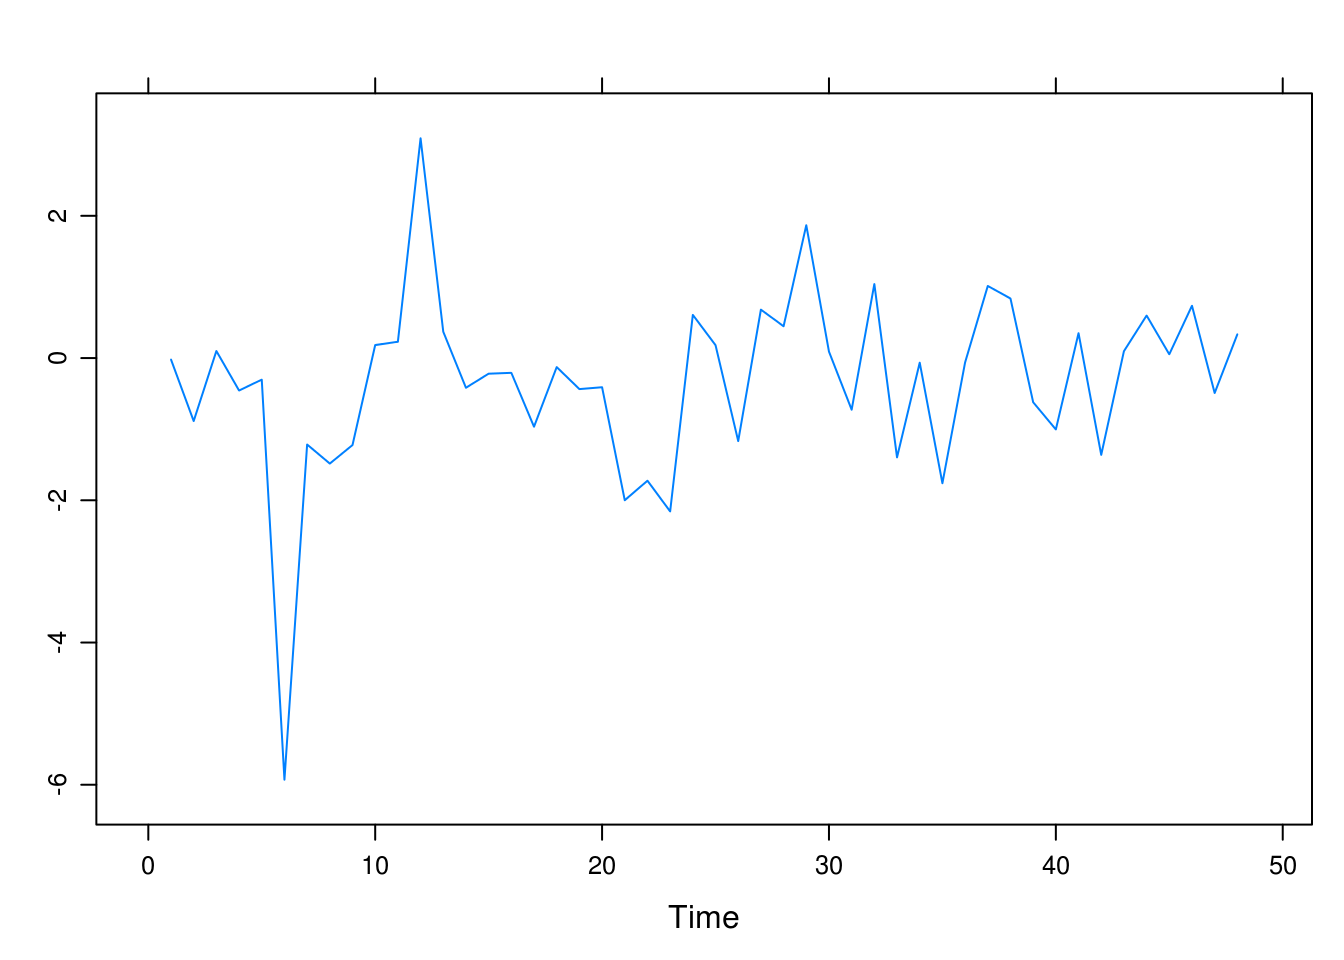
\includegraphics{TSAsolutions_files/figure-latex/unnamed-chunk-5-1.pdf}
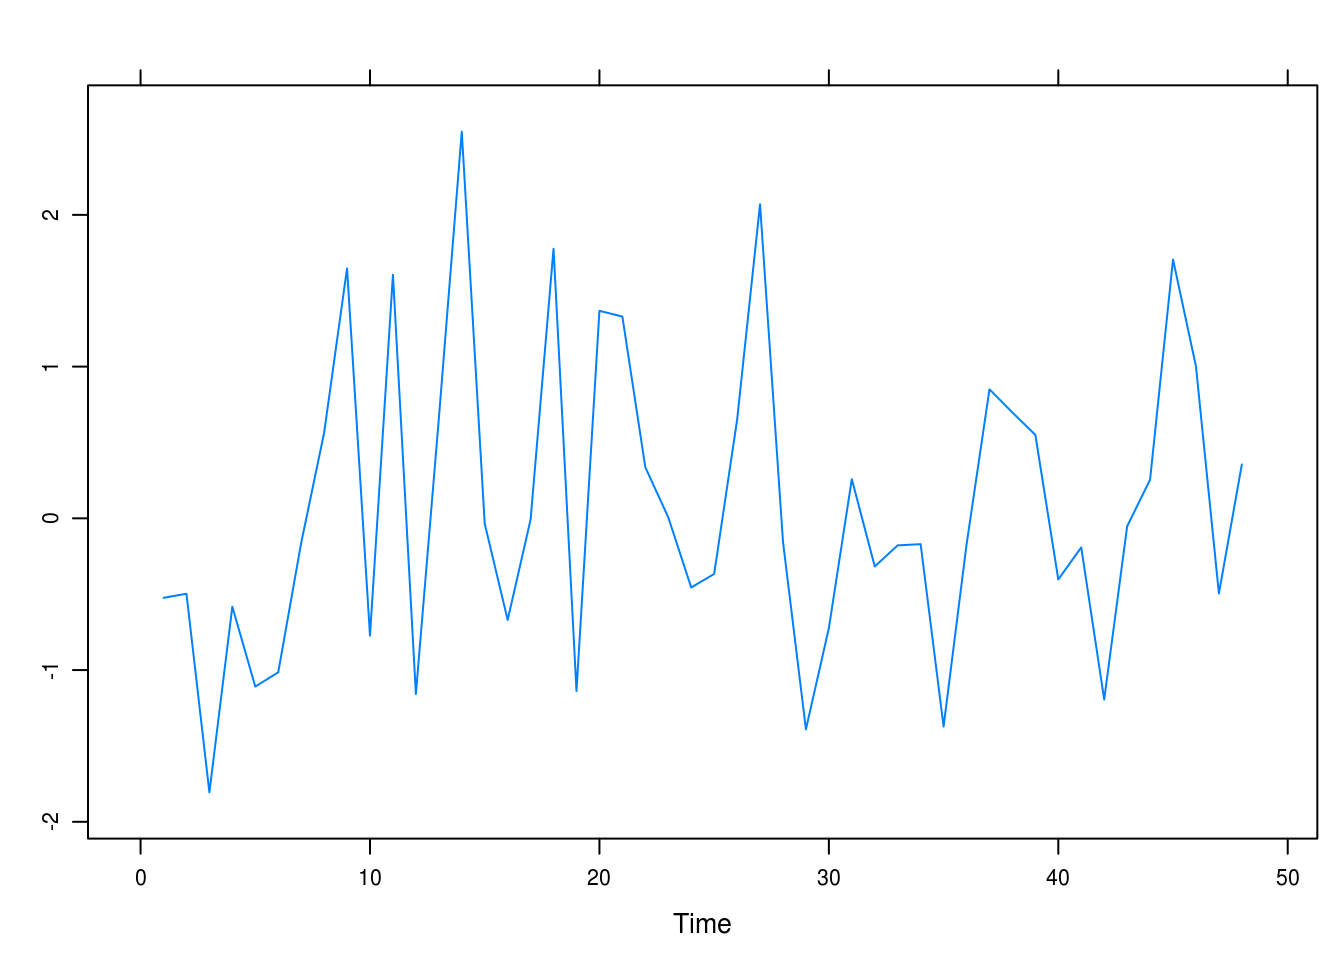
\includegraphics{TSAsolutions_files/figure-latex/unnamed-chunk-5-2.pdf}

As far as we can tell there is no discernable pattern here.

\section{\texorpdfstring{Random, \(\chi^2\)-distributed time
series}{Random, \textbackslash{}chi\^{}2-distributed time series}}\label{random-chi2-distributed-time-series}

\begin{quote}
Simulate a completely random process of length 48 with independent,
chi-square distributed values, each with 2 degrees of freedom. Display
the time series plot. Does it look ``random'' and nonnormal? Repeat this
exercise several times with a new simulation each time.
\end{quote}

\begin{Shaded}
\begin{Highlighting}[]
\KeywordTok{xyplot}\NormalTok{(}\KeywordTok{as.ts}\NormalTok{(}\KeywordTok{rchisq}\NormalTok{(}\DecValTok{48}\NormalTok{, }\DecValTok{2}\NormalTok{)))}
\KeywordTok{xyplot}\NormalTok{(}\KeywordTok{as.ts}\NormalTok{(}\KeywordTok{rchisq}\NormalTok{(}\DecValTok{48}\NormalTok{, }\DecValTok{2}\NormalTok{)))}
\end{Highlighting}
\end{Shaded}

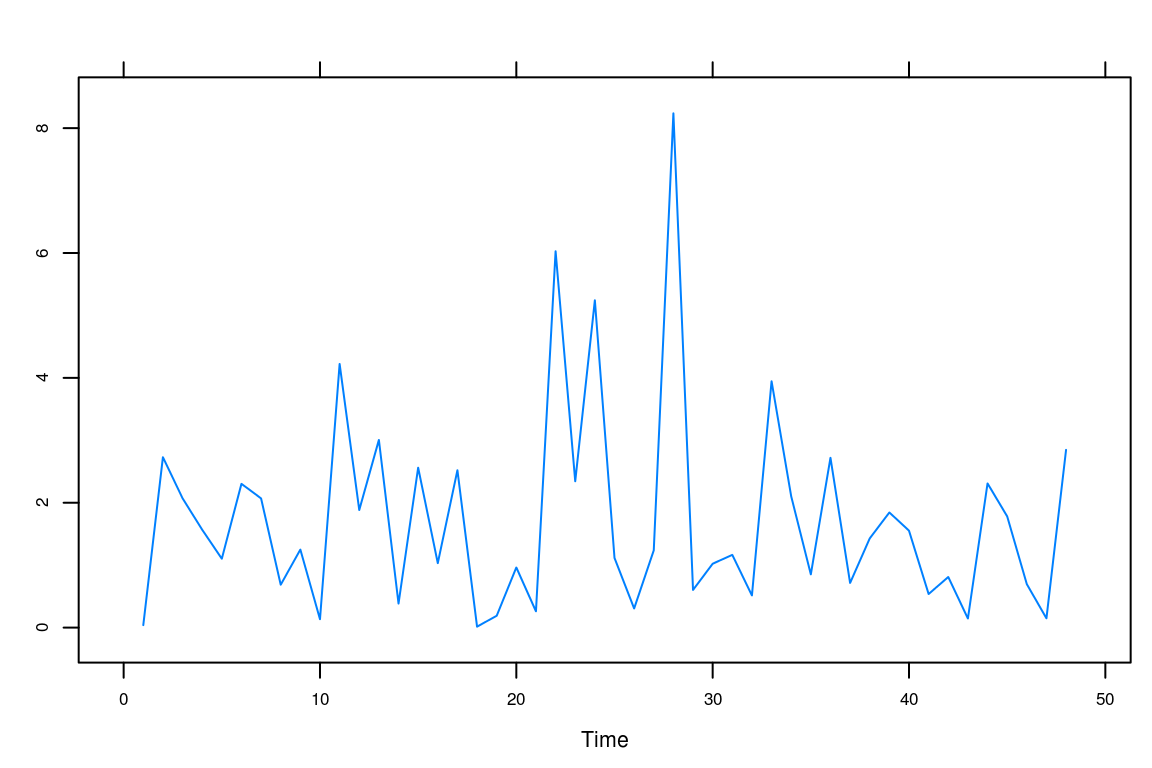
\includegraphics{TSAsolutions_files/figure-latex/unnamed-chunk-6-1.pdf}
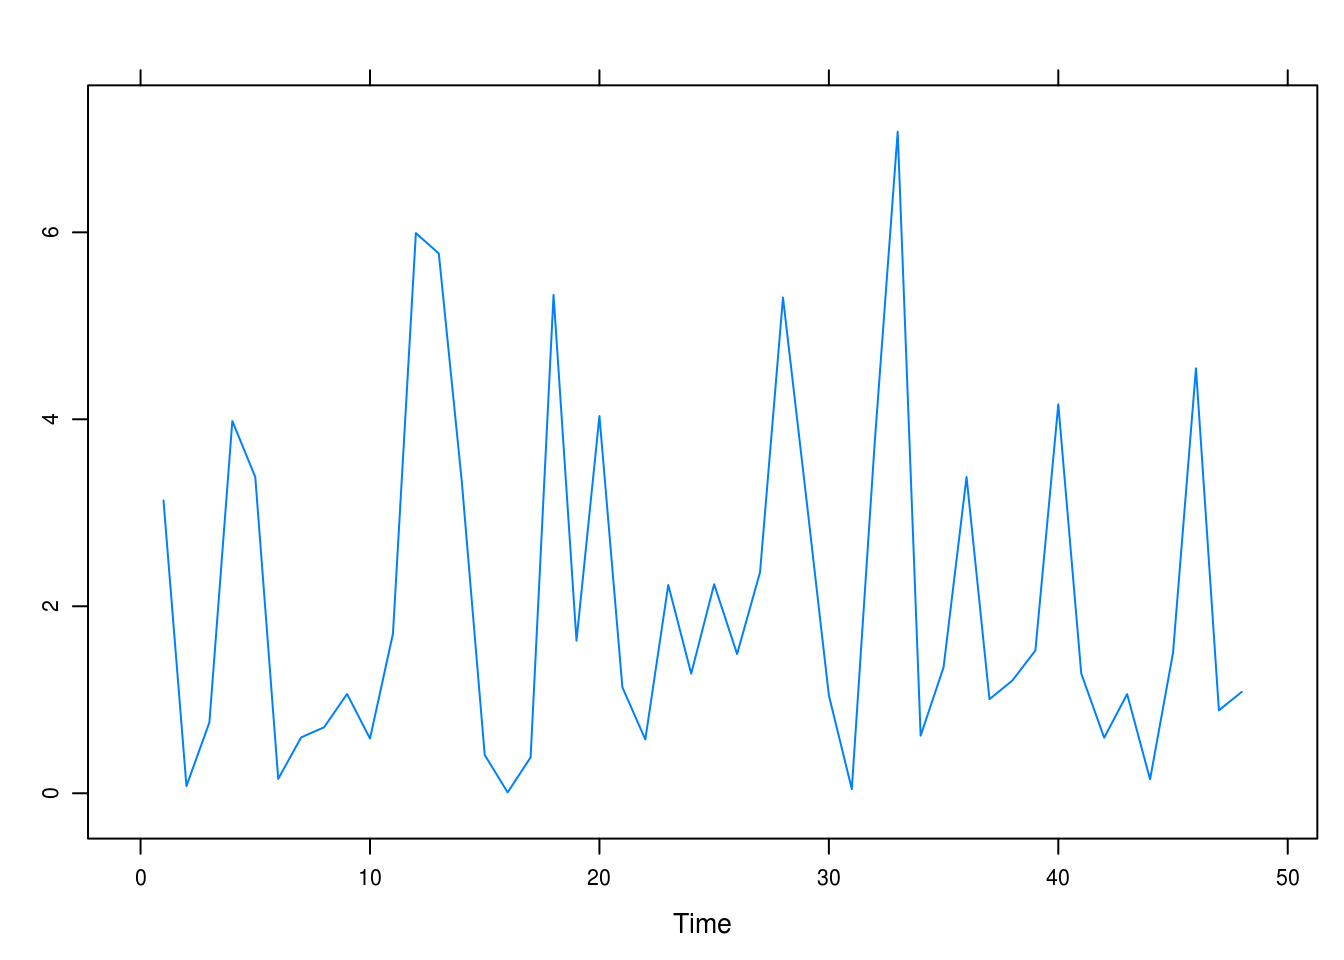
\includegraphics{TSAsolutions_files/figure-latex/unnamed-chunk-6-2.pdf}

The process appears random, though non-normal.

\section{\texorpdfstring{\emph{t}(5)-distributed, random
values}{t(5)-distributed, random values}}\label{t5-distributed-random-values}

\begin{quote}
Simulate a completely random process of length 48 with independent,
t-distributed values each with 5 degrees of freedom. Construct the time
series plot. Does it look ``random'' and nonnormal? Repeat this exercise
several times with a new simulation each time.
\end{quote}

\begin{Shaded}
\begin{Highlighting}[]
\KeywordTok{xyplot}\NormalTok{(}\KeywordTok{as.ts}\NormalTok{(}\KeywordTok{rt}\NormalTok{(}\DecValTok{48}\NormalTok{, }\DecValTok{5}\NormalTok{)))}
\end{Highlighting}
\end{Shaded}

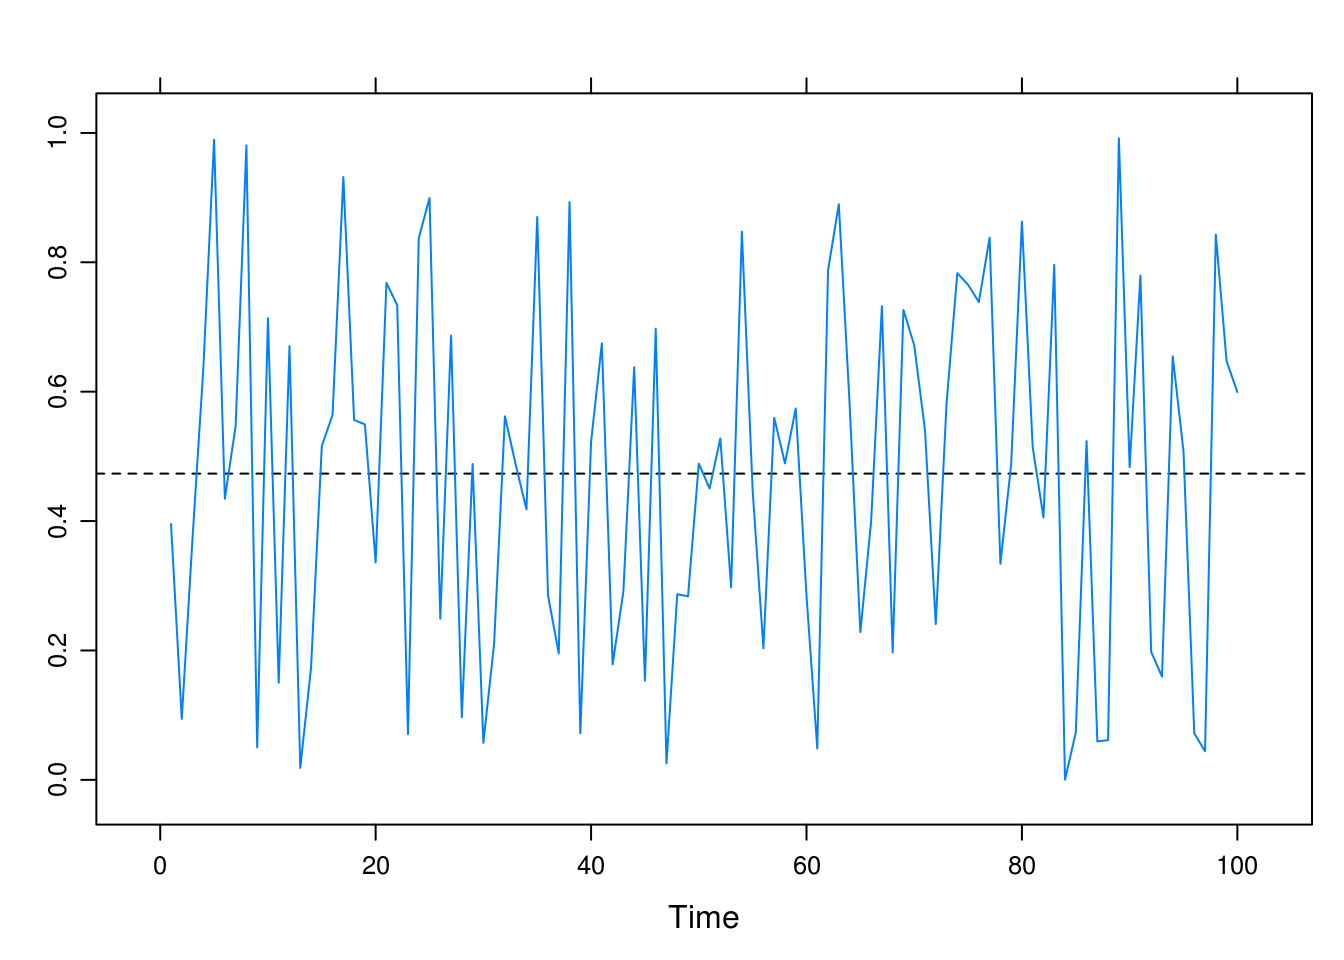
\includegraphics{TSAsolutions_files/figure-latex/unnamed-chunk-7-1.pdf}

\begin{Shaded}
\begin{Highlighting}[]
\KeywordTok{xyplot}\NormalTok{(}\KeywordTok{as.ts}\NormalTok{(}\KeywordTok{rt}\NormalTok{(}\DecValTok{48}\NormalTok{, }\DecValTok{5}\NormalTok{)))}
\end{Highlighting}
\end{Shaded}

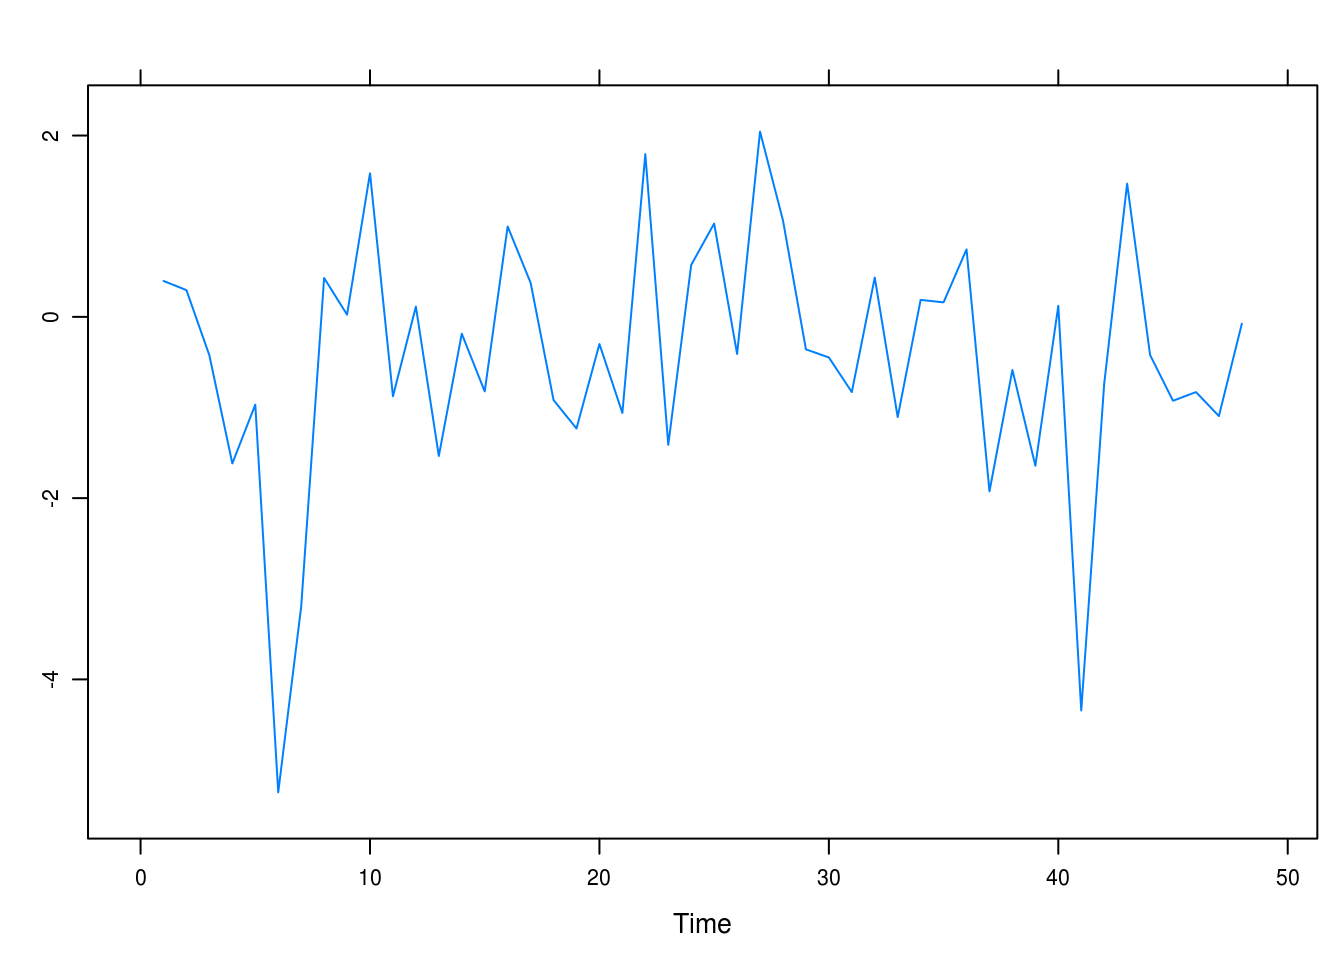
\includegraphics{TSAsolutions_files/figure-latex/unnamed-chunk-7-2.pdf}

It looks random but not normal, though it should be approximately so,
considering the distribution that we have sampled from.

\section{Dubuque temperature series}\label{dubuque-temperature-series}

\begin{quote}
Construct a time series plot with monthly plotting symbols for the
Dubuque temperature series as in Exhibit 1.7, on page 6. The data are in
the file named tempdub.
\end{quote}

\begin{Shaded}
\begin{Highlighting}[]
\KeywordTok{data}\NormalTok{(tempdub)}
\KeywordTok{xyplot}\NormalTok{(tempdub, }\DataTypeTok{ylab =} \StringTok{"Temperature"}\NormalTok{, }\DataTypeTok{xlab =} \StringTok{"Year"}\NormalTok{)}
\end{Highlighting}
\end{Shaded}

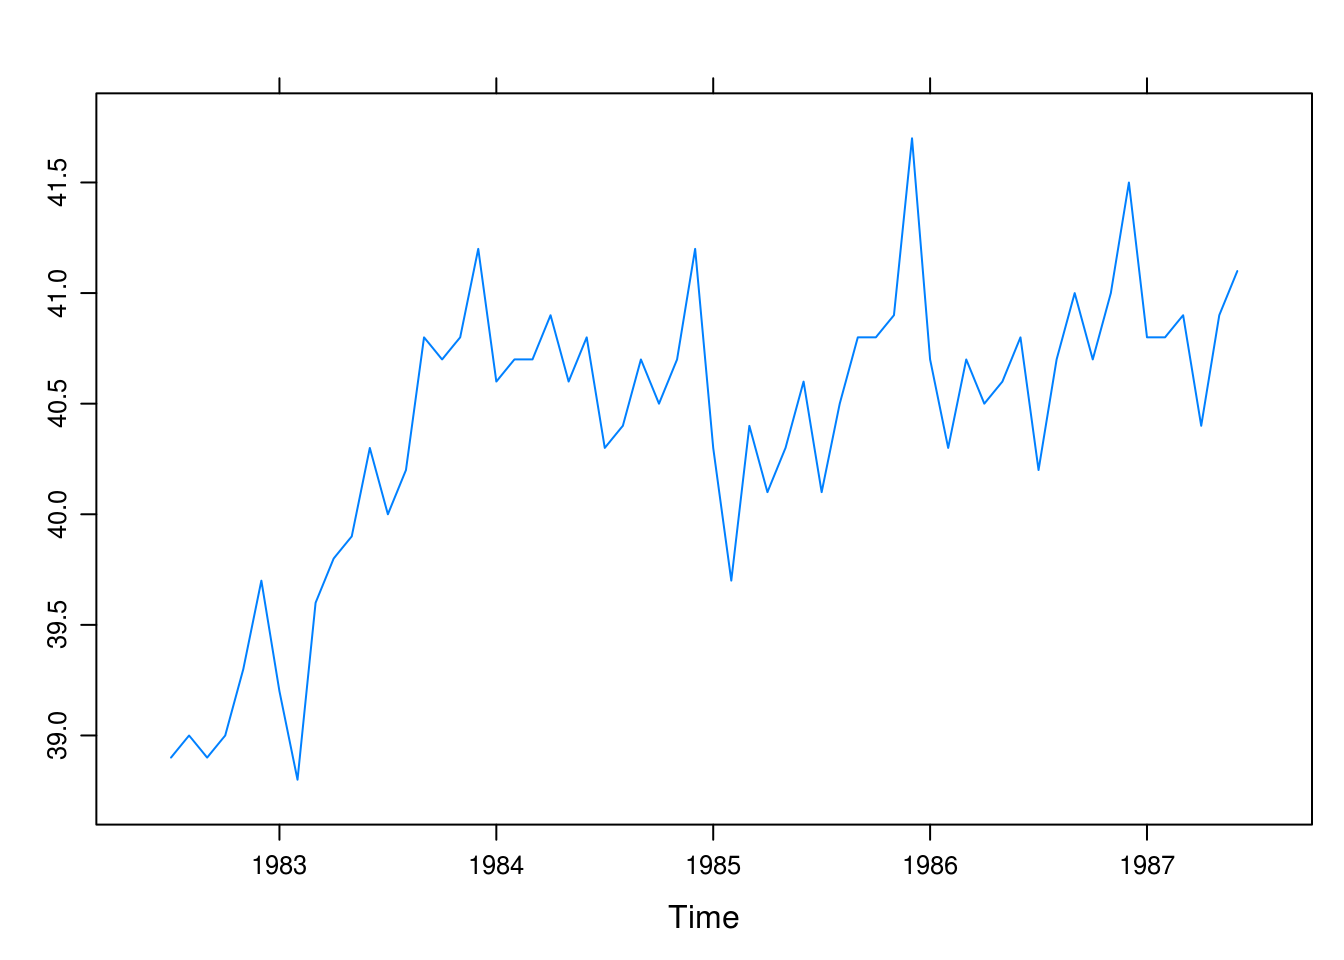
\includegraphics{TSAsolutions_files/figure-latex/unnamed-chunk-8-1.pdf}

\chapter{Fundamental concepts}\label{fundamental-concepts}

\section{Basic properties of expected value and
covariance}\label{basic-properties-of-expected-value-and-covariance}

\subsection*{a}\label{a}
\addcontentsline{toc}{subsection}{a}

\begin{align}
    \text{Cov}[X,Y] & = \text{Corr}[X,Y]\sqrt{Var[X]Var[Y]}\\
                    & = 0.25 \sqrt{9 \times 4} = 1.5 \\
    \text{Var}[X,Y] & = Var[X]+Var[Y]+2Cov[X,Y]\\
                    & = 9 + 4 + 2 \times 3 = 16\\
    \end{align}

\subsection*{b}\label{b}
\addcontentsline{toc}{subsection}{b}

\[\text{Cov}[X, X+Y] = \text{Cov}[X,X] + \text{Cov}[X,Y] =
  \text{Var}[X] + \text{Cov}[X,Y] = 9 + 1.5 = 10.5\]

\subsection*{c}\label{c}
\addcontentsline{toc}{subsection}{c}

\begin{align}
\text{Corr}[X+Y, X-Y] = & \text{Corr}[X,X] + \text{Corr}[X,-Y] +
                          \text{Corr}[Y,X] + \text{Corr}[Y,-Y] \\
                      = & \text{Corr}[Y,X] + \text{Corr}[Y,-Y] \\
                      = & 1 - 0.25 + 0.25 -1 \\
                      = & 0 \\
\end{align}

\section{Dependence and covariance}\label{dependence-and-covariance}

\begin{gather*}
\text{Cov}[X+Y,X-Y] = \text{Cov}[X,X] + \text{Cov}[X,-Y] +
  \text{Cov}[Y,X] + \text{Cov}[Y, -Y] = \\
Var[X] - Cov[X,Y] + Cov[X,Y] - Var[Y] = 0
\end{gather*}

since \(Var[X] = Var[Y]\).

\section{Strict and weak
stationarity}\label{strict-and-weak-stationarity}

\subsection*{a}\label{a-1}
\addcontentsline{toc}{subsection}{a}

We have that

\begin{gather*}
P(Y_{t_1}, Y_{t_2}, \dots, Y_{t_n}) = \\
  P(X_1, X_2, \dots, X_n) = \\
  P(Y_{t_1 - k}, Y_{t_2 - k}, \dots, Y_{t_n - k}),
\end{gather*}

which satisfies our requirement for strict stationarity.

\subsection*{b}\label{b-1}
\addcontentsline{toc}{subsection}{b}

The autocovariance is given by

\begin{gather*}
  \gamma_{t,s}=\text{Cov}[Y_t, Y_s] = \text{Cov}[X,X] = \text{Var}[X] = \sigma^2.
\end{gather*}

\subsection*{c}\label{c-1}
\addcontentsline{toc}{subsection}{c}

\begin{Shaded}
\begin{Highlighting}[]
\KeywordTok{library}\NormalTok{(lattice)}
\NormalTok{tstest <-}\StringTok{ }\KeywordTok{ts}\NormalTok{(}\KeywordTok{runif}\NormalTok{(}\DecValTok{100}\NormalTok{))}

\NormalTok{lattice::}\KeywordTok{xyplot}\NormalTok{(tstest,}
                \DataTypeTok{panel =} \NormalTok{function(x, y, ...) \{}
                  \KeywordTok{panel.abline}\NormalTok{(}\DataTypeTok{h =} \KeywordTok{mean}\NormalTok{(y), }\DataTypeTok{lty =} \DecValTok{2}\NormalTok{)}
                  \KeywordTok{panel.xyplot}\NormalTok{(x, y, ...)}
                \NormalTok{\})}
\end{Highlighting}
\end{Shaded}

\begin{figure}[htbp]
\centering
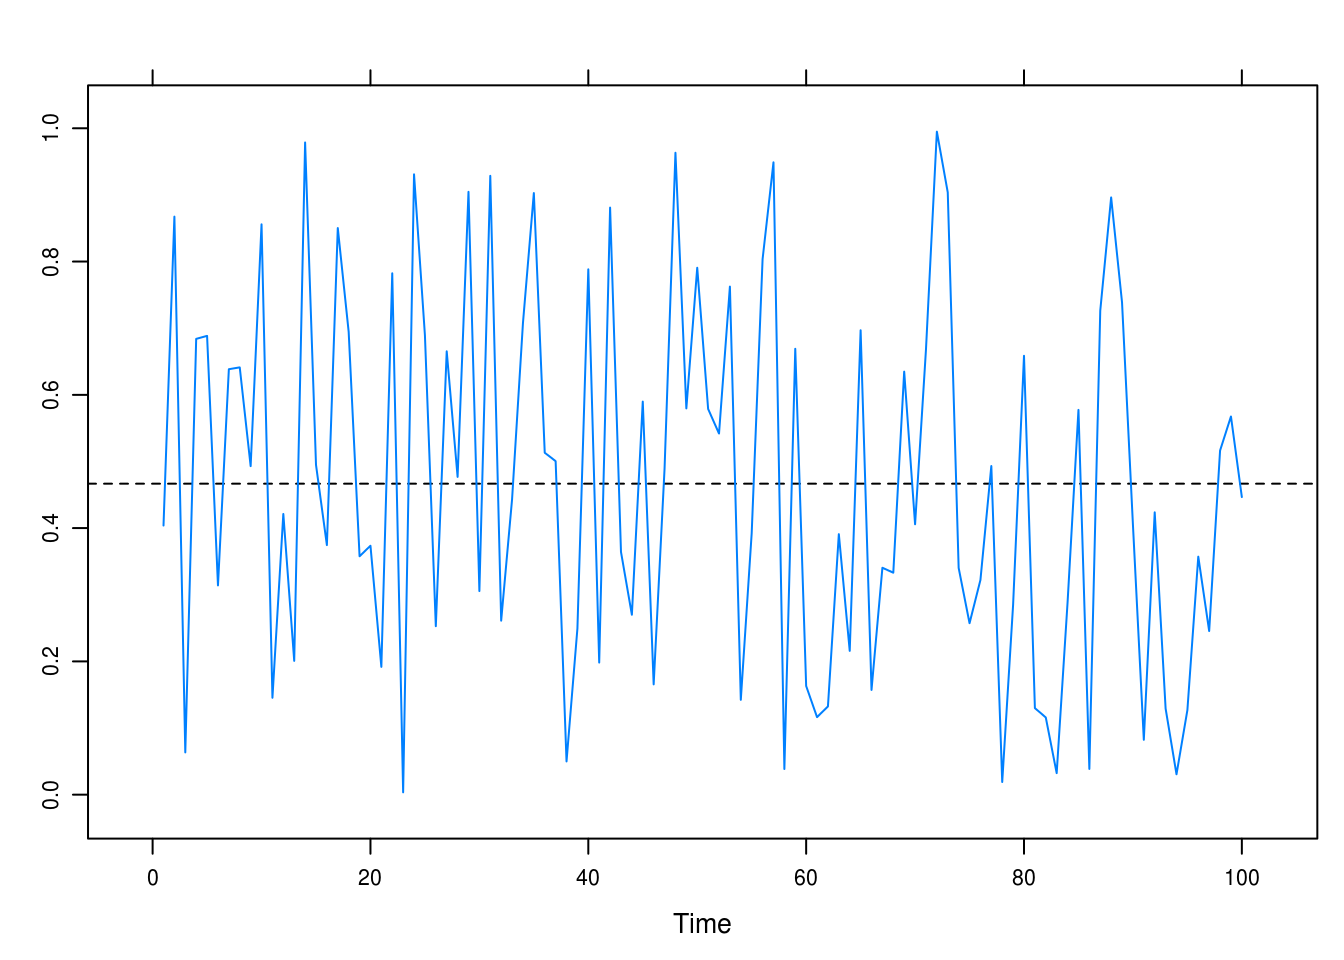
\includegraphics{TSAsolutions_files/figure-latex/unnamed-chunk-9-1.pdf}
\caption{\label{fig:unnamed-chunk-9}A white noise time series: no drift,
independence between observations.}
\end{figure}

\section{Zero-mean white noise}\label{zero-mean-white-noise}

\subsection*{a}\label{a-2}
\addcontentsline{toc}{subsection}{a}

\begin{gather*}
  E[Y_t] = E[e_t+\theta e_{t-1}] = E[e_t] + \theta E[e_{t-1}] = 0 + 0 = 0\\
  V[Y_t] = V[e_t + \theta e_{t-1}] =  V[e_t] + \theta^2 V[e_{t-1}] = \sigma_e^2 + \theta^2 \sigma_e^2 = \sigma_2^2(1 + \theta^2)\\
\end{gather*}

For \(k = 1\) we have

\begin{gather*}
  C[e_t + \theta e_{t-1}, e_{t-1} + \theta e_{t-2}] = \\
  C[e_t,e_{t-1}] + C[e_t, \theta e_{t-2}] + C[\theta e_{t-1}, e_{t-1}] + C[\theta e_{t-1}, \theta e_{t-2}] = \\
  0 + 0 + \theta V[e_{t-1}] + 0 = \theta \sigma_e^2,\\
  \text{Corr}[Y_t, Y_{t-k}] = \frac{\theta \sigma_e^2}{\sqrt{(\sigma_e^2(1+\theta^2))^2}} = \frac{\theta }{1+\theta^2}
\end{gather*}

and for \(k = 0\) we get

\begin{gather*}
  \text{Corr}[Y_t, Y_{t-k}] = \text{Corr}[Y_t, Y_t] = 1
\end{gather*}

and, finally, for \(k > 0\):

\begin{gather*}
  C[e_t + \theta e_{t-1}, e_{t-k} + \theta e_{t-k-1}] = \\
  C[e_t, e_{t-k}] + C[e_t, e_{t-1-k}] + C[\theta e_{t-1}, e_{t-k}] + C[\theta e_{t-1}, \theta e_{t-1-k}] = 0
\end{gather*}

given that all terms are independent. Taken together, we have that

\begin{gather*} \text{Corr}[Y_t, Y_{t-k}] =
  \begin{cases}
    1                            & \quad \text{for } k = 0\\
    \frac{\theta}{1 + \theta^2}  & \quad \text{for } k = 1\\
    0                            & \quad \text{for } k > 1
  \end{cases}.
\end{gather*}

And, as required,

\begin{gather*}
  \text{Corr}[Y_t, Y_{t-k}] =
  \begin{cases}
    \frac{3}{1+3^2} = \frac{3}{10} & \quad \text{if } \theta = 3\\
    \frac{1/3}{1 + (1/3)^2} = \frac{1}{10/3} = \frac{3}{10}  & \quad \text{if } \theta = 1/3
  \end{cases}.
\end{gather*}

\subsection*{b}\label{b-2}
\addcontentsline{toc}{subsection}{b}

No, probably not. Given that \(\rho\) is standardized, we will not be
able to detect any difference in the variance regardless of the values
of k.

\section{Zero-mean stationary series}\label{zero-mean-stationary-series}

\subsection*{a}\label{a-3}
\addcontentsline{toc}{subsection}{a}

\[\mu_t = E[Y_t] = E[5 + 2t + X_t] = 5 + 2E[t] + E[X_t] = 5 + 2t + 0 = 2t + 5\]

\subsection*{b}\label{b-3}
\addcontentsline{toc}{subsection}{b}

\[ \gamma_k = \text{Corr}[5+2t+X_t, 5+2(t-k)+X_{t-k}] =
  \text{Corr}[X_t, X_{t-k}]\]

\subsection*{c}\label{c-2}
\addcontentsline{toc}{subsection}{c}

No, the mean function (\(\mu_t\)) is constant and the aurocovariance
(\(\gamma_{t,t-k}\)) free from \(t\).

\section{Stationary time series}\label{stationary-time-series}

\subsection*{a}\label{a-4}
\addcontentsline{toc}{subsection}{a}

\begin{gather*}\text{Cov}[a + X_t, b + X_{t-k}] =\text{Cov}[X_t, X_{t-k}],\end{gather*}

which is free from \(t\) for all \(k\) because \(X_t\) is stationary.

\subsection*{b}\label{b-4}
\addcontentsline{toc}{subsection}{b}

\begin{gather*}
  \mu_t = E[Y_t] = 
    \begin{cases}
      E[X_t]       & \quad \text{for odd } t\\
      3 + E[X_t]   & \quad \text{for even } t\\
    \end{cases}.
\end{gather*}

Since \(\mu_t\) varies depending on \(t\), \(Y_t\) is not stationary.

\section{First and second-order difference
series}\label{first-and-second-order-difference-series}

\subsection*{a}\label{a-5}
\addcontentsline{toc}{subsection}{a}

\begin{gather*}\mu_t = E[W_t] = E[Y_t - Y_{t-1}] = E[Y_t] - E[Y_{t-1}] = 0\end{gather*}

because \(Y_t\) is stationary.

\begin{gather*}
  \text{Cov}[W_t] = \text{Cov}[Y_t - Y_{t-1}, Y_{t-k} - Y_{t-1-k}] = \\
  \text{Cov}[Y_t, Y_{t-k}] + \text{Cov}[Y_t, Y_{t-1-k}] + \text{Cov}[-Y_{t-k}, Y_{t-k}] + \text{Cov}[-Y_{t-k}, -Y_{t-1-k}]=\\
  \gamma_k-\gamma_{k+1}-\gamma_{k-1}+\gamma_{k} = 2 \gamma_k - \gamma_{k+1} - \gamma_{k-1}. \quad \square
\end{gather*}

\subsection*{b}\label{b-5}
\addcontentsline{toc}{subsection}{b}

In (a), we discovered that the difference between two stationary
processes, \(\triangledown Y_t\) itself was stationary. It follows that
the difference between two of these differences, \(\triangledown^2Y_t\)
is also stationary.

\section{Generalized difference
series}\label{generalized-difference-series}

\begin{align}
  E[W_t] & = c_1E[Y_t]+c_2E[Y_t] + \dots + c_n E[Y_t]\\
         & = E[Y_t](c_1 + c_2 + \dots + c_n),
\end{align}

and thus the expected value is constant. Moreover,

\begin{align}
  \text{Cov}[W_t] & = \text{Cov}[c_1 Y_t + c_2 Y_{t-1} + \dots + c_n Y_{t-k}, c_1 Y_{t-k} + c_2 Y_{t-k-1} + \dots + c_n Y_{t-k-n}] \\
                  & = \sum_{i=0}^n \sum_{j=0}^n c_i c_j \text{Cov}[Y_{t-j}Y_{t-i-k}] \\
                  & = \sum_{i=0}^n \sum_{j=0}^n c_i c_j \gamma_{j-k-i},
\end{align}

which is free of \(t\); consequently, \(W_t\) is stationary.

\section{Zero-mean stationary difference
series}\label{zero-mean-stationary-difference-series}

\subsection*{a}\label{a-6}
\addcontentsline{toc}{subsection}{a}

\begin{gather*}
  E[Y_t] = \beta_0 + \beta_1 t + E[X_t] = \beta_0 + \beta_1 t + \mu_{t_x},
\end{gather*}

which is not free of \(t\) and hence \emph{not} stationary.

\begin{gather*}
  \text{Cov}[Y_t] = \text{Cov}[X_t, X_t-1] = \gamma_{t-1}
\end{gather*}

\begin{gather*}
  E[W_t] = E[Y_t - Y_{t-1}] = E[\beta_0 + \beta_1 t + X_t - (\beta_0 + \beta_1(t-1) + X_{t-1})] =\\
  \beta_0 + \beta_1 t - \beta_0 - \beta_1 t + \beta_1  = \beta_1,
\end{gather*}

is free of \(t\) and, furthermore, we have

\begin{gather*}
  \text{Cov}[W_t] = \text{Cov}[\beta_0 + \beta_1 t + X_t, \beta_0 + \beta_1 (t-1) + X_{t-1}] =\\
  \text{Cov}[X_t, X_{t-1}] = \gamma_k,  
\end{gather*}

which is also free of \(t\), thereby proving that \(W_t\) is stationary.

\subsection*{b}\label{b-6}
\addcontentsline{toc}{subsection}{b}

\begin{gather*}
  E[Y_t] = E[\mu_t + X_t] = \mu_t + \mu_t = 0 + 0 = 0, \quad \text{and}\\
  \text{Cov}[Y_t] = \text{Cov}[\mu_t + X_t, \mu_{t-k} + X_{t-k}] = \text{Cov}[X_t, X_{t-k}] = \gamma_k
\end{gather*}

\begin{gather*}
  \triangledown^m Y_t = \triangledown(\triangledown^{m−1}Y_t)
\end{gather*}

\emph{Currently unsolved.}

\section{Zero-mean, unit-variance
process}\label{zero-mean-unit-variance-process}

\subsection*{a}\label{a-7}
\addcontentsline{toc}{subsection}{a}

\begin{gather*}
  \mu_t = E[Y_t] = E[\mu_t + \sigma_t X_t] = \mu_t + \sigma_t E[X_t] = \mu_t + \sigma_t \times 0 = \mu_t\\
  \gamma_{t,t-k} = \text{Cov}[Y_t] = \text{Cov}[\mu_t + \sigma_t X_t, \mu_{t-k} + \sigma_{t-k} X_{t-k}] = 
    \sigma_t \sigma_{t-k} \text{Cov}[X_t, X_{t-k}] = \sigma_t \sigma_{t-k} \rho_k
\end{gather*}

\subsection*{b}\label{b-7}
\addcontentsline{toc}{subsection}{b}

First, we have

\begin{gather*}
  \text{Var}[Y_t] = \text{Var}[\mu_t + \sigma_t X_t] = 0 + \sigma_t^2 \text{Var}[X_t] = \sigma_t^2 \times 1 = \sigma_t^2
\end{gather*}

since \(\{X_t\}\) has unit-variance. Futhermore,

\begin{gather*}
  \text{Corr}[Y_t, Y_{t-k}] = \frac{\sigma_t \sigma_{t-k} \rho_k}{\sqrt{\text{Var}[Y_t]\text{Var}[Y_{t-k}]}} = 
    \frac{\sigma_t \sigma_{t-k}\rho_k}{\sigma_t \sigma_{t-k}} = \rho_k,
\end{gather*}

which depends only on the time lag, \(k\). However, \(\{Y_t\}\) is not
necessarily stationary since \(\mu_t\) may depend on \(t\).

\subsection*{c}\label{c-3}
\addcontentsline{toc}{subsection}{c}

Yes, \(\rho_k\) might be free from \(t\) but if \(\sigma_t\) is not, we
will have a non-stationary time series with autocorrelation free from
\(t\) and constant mean.

\section{Drift}\label{drift}

\subsection*{a}\label{a-8}
\addcontentsline{toc}{subsection}{a}

\begin{gather*}
  \text{Cov}[X_t, X_{t-k}] = \gamma_k\\
  E[X_t] = 3t
\end{gather*}

\(\{X_t\}\) is not stationary because \(\mu_t\) varies with \(t\).

\subsection*{b}\label{b-8}
\addcontentsline{toc}{subsection}{b}

\begin{gather*}
  E[Y_t] = 3 - 3t+E[X_t] = 7 - 3t - 3t = 7\\
  \text{Cov}[Y_t, Y_{t-k}] = \text{Cov}[7-3t+X_t,7-3(t-k)+X_{t-k}] = \text{Cov}[X_t, X_{t-k}] = \gamma_k
\end{gather*}

Since the mean function of \(\{Y_t\}\) is constant (7) and its
autocovariance free of \(t\), \(\{Y_t\}\) is stionary.

\section{Periods}\label{periods}

\begin{gather*}
  E[Y_t] = E[e_t - e_{t-12}] = E[e_t] - E[e_{t-12}] = 0\\
  \text{Cov}[Y_t, Y_{t-k}] = \text{Cov}[e_t - e_{t-12}, e_{t-k} - e_{t-12-k}] =\\
  \text{Cov}[e_t, e_{t-k}] - \text{Cov}[e_t, e_{t-12-k}] - \text{Cov}[e_{t-12}, e_{t-k}] + \text{Cov}[e_{t-12}, e_{t-12-k}]
\end{gather*}

Then, as required, we have

\begin{gather*} \text{Cov}[Y_t, Y_{t-k}] =
  \begin{cases}
    \text{Cov}[e_t, e_{t-12}] - \text{Cov}[e_t, e_t] -\\ \text{Cov}[e_{t-12}, e_{t-12}] + \text{Cov}[e_{t-12},e_t] =\\
      \text{Var}[e_t] - \text{Var}[e_{t-12}] \neq 0 & \quad \text{for }  k=12\\
      \\
    \text{Cov}[e_t, e_{t-k}] - \text{Cov}[e_t, e_{t-12-k}] -\\ \text{Cov}[e_{t-12}, e_{t-k}] + \text{Cov}[e_{t-12}, e_{t-12-k}] =\\
    0 + 0 + 0 + 0 = 0 & \quad \text{for } k \neq 12
  \end{cases}
\end{gather*}

\section{Drift, part 2}\label{drift-part-2}

\subsection*{a}\label{a-9}
\addcontentsline{toc}{subsection}{a}

\begin{gather*}
  E[Y_t] = E[e_t - \theta e_{t-1}^2] = E[e_t] - \theta E[e_{t-1}^2] = 0 - \theta \text{Var}[e_{t-1}] = -\theta \sigma_e^2
\end{gather*}

And thus the requirement of constant variance is fulfilled. Moreover,

\begin{gather*}
  \text{Var}[Y_t] = \text{Var}[e_t-\theta e_{t-1}^2] = \text{Var}[e_t] + \theta^2 \text{Var}[e_{t-1}^2] = \sigma_e^2 + \theta^2 (E[e_{t-1}^4] - E[e_{t-1}^2]^2),
\end{gather*}

where

\begin{gather*}
  E[e_{t-1}^4] = 3\sigma_e^4 \quad \text{and} \quad E[e_{t-1}^2 ]^2 = \sigma_e^4,
\end{gather*}

gives us

\begin{gather*}
  \text{Var}[Y_t] = \sigma_e^2 + \theta(3\sigma_e^4 - \sigma_e^2) = \sigma_e^2 + 2 \theta^2 \sigma_e^4
\end{gather*}

and

\begin{gather*}
  \text{Cov}[Y_t, Y_{t-1}] = \text{Cov}[e_t - \theta e_{t-1}^2, e_{t-1} - \theta e_{t-2}^2] = \\
  \text{Cov}[e_t, e_{t-1}] + \text{Cov}[e_t, - \theta e_{t-2}^2] + \text{Cov}[- \theta e_{t-1}^2, e_{t-1}]
    \text{Cov}[-\theta e_{t-1}^2, - \theta e_{t-2}^2] =\\
  \text{Cov}[e_t, e_{t-1}] - \theta \text{Cov}[e_t, e_{t-2}^2] - \theta \text{Cov}[e_{t-1}^2, e_{t-1}] +
    \theta^2 \text{Cov}[e_{t-1}^2, e_{t-2}^2] = \\
  -\theta \text{Cov}[e_{t-1}^2, e_{t-1}] = -\theta (E[e_{t-1}^3] + \mu_{t-1} + \mu_t) = 0
\end{gather*}

which means that the autocorrelation function \(\gamma_{t,s}\) also has
to be zero.

\subsection*{b}\label{b-9}
\addcontentsline{toc}{subsection}{b}

The autocorrelation of \(\{Y_t\}\) is zeor and its mean function is
constant, thus \(\{Y_t\}\) must be stationary.

\section{Stationarity, again}\label{stationarity-again}

\subsection*{a}\label{a-10}
\addcontentsline{toc}{subsection}{a}

\begin{gather*}
  E[Y_t]= E[\theta_0 +  t e_t] = \theta_0 + E[e_t] = \theta_0+t \times 0 = \theta_0\\
\text{Var}[Y_t] = \text{Var}[\theta_0] + \text{Var}[t e_t] = 0 + t^2\sigma_e^2 = t^2\sigma_e^2
\end{gather*}

So \(\{Y_t\}\) is not stationary.

\subsection*{b}\label{b-10}
\addcontentsline{toc}{subsection}{b}

\begin{gather*}
  E[W_t] = E[\triangledown Y_t] = E[\theta_0 + te_t - \theta_0 - (t-1)e_{t-1}] =
    tE[e_t] - tE[e_{t-1} + E[e_{t-1}] = 0 \\
  \text{Var}[\triangledown Y_t] = \text{Var}[t e_t] = - \text{Var}[(t-1)e_{t-1}] = 
    t^2 \sigma_e^2 - (t-1)^2 \sigma_e^2 = \sigma_e^2 (t^2 - t^2 + 2t - 1) = (2t-1)\sigma_e^2,
\end{gather*}

which varies with \(t\) and means that \(\{W_t\}\) is not stationary.

\subsection*{c}\label{c-4}
\addcontentsline{toc}{subsection}{c}

\begin{gather*}
  E[Y_t] = E[e_t e_{t-1}] = E[e_t] E[e_{t-1}] = 0\\
  \text{Cov}[Y_t, Y_{t-1}] = \text{Cov}[e_t e_{t-1}, e_{t-1} e_{t-2}] = E[(e_t e_{t-1} - \mu_t^2)(e_{t-1} e_{t-2} - \mu_t^2)] =\\
  E[e_t]E[e_{t-1}]E[e_{t-1}]E[e_{t-2}] = 0
\end{gather*}

Both the covariance and the mean function are zero, hence the process is
stationary.

\section{Random variable, zero mean}\label{random-variable-zero-mean}

\subsection*{a}\label{a-11}
\addcontentsline{toc}{subsection}{a}

\(E[Y_t] = (-1)^tE[X] = 0\)

\subsection*{b}\label{b-11}
\addcontentsline{toc}{subsection}{b}

\(\text{Cov}[Y_t, Y_{t-k}] = \text{Cov}[(-1)^tX, (-1)^{t-k}X] = (-1)^{2t-k}\text{Cov}[X, X] = (-1)^k \text{Var}[X] = (-1)^k\sigma_t^2\)

\subsection*{c}\label{c-5}
\addcontentsline{toc}{subsection}{c}

Yes, the covariance is free of \(t\) and the mean is constant.

\section{Mean and variance}\label{mean-and-variance}

\begin{gather*}
  E[Y_t] = E[A + X_t] = E[A] + E[X_t] = \mu_A + \mu_X\\
  \text{Cov}[Y_t, Y_{t-k}] = \text{Cov}[A + X_t, A+ X_{t-k}] = \\
  \text{Cov}[A, A] + \text{Cov}[A, X_{t-k}] + \text{Cov}[X_t, A] + \text{Cov}[X_t, X_{t-k}] = \sigma_A^2 + \gamma_{k_k}
\end{gather*}

\section{Variance of sample mean}\label{variance-of-sample-mean}

\begin{gather*}
  \text{Var}[\bar{Y}] = \text{Var}\left[ \frac{1}{n} \sum_{t=1}^n Y_t \right] = \frac{1}{n^2} \text{Var}\left[ \sum_{t=1}^n Y_t \right] = \\
  \frac{1}{n^2}\text{Cov}\left[ \sum_{t=1}^n Y_t, \sum_{s=1}^n Y_s \right] = \frac{1}{n^2} \sum_{t=1}^n \sum_{s=1}^n \gamma_{t-s}
\end{gather*}

Setting \(k = t-s, j = t\) gives us

\begin{gather*}
  \text{Var}[\bar{Y}] = \frac{1}{n^2} \sum_{j=1}^n \sum_{j-k=1}^n \gamma_k = \frac{1}{n^2} \sum_{j=1}^n \sum_{j=k+1}^{n+k} \gamma_k = \\
  \frac{1}{n^2} \left( \sum_{k=1}^{n-1} \sum_{j=k+1}^{n} \gamma_k + \sum_{k=-n+1}^0 \sum_{j=1}^{n+k} \gamma_k \right) = \\
  \frac{1}{n^2} \left( \sum_{k=1}^{n-1} (n-k)\gamma_k + \sum_{k=-n+1}^0 (n+k)\gamma_k \right) = \\
  \frac{1}{n^2} \sum_{k=-n+1}^{n-1} \left( (n-k)\gamma_k + (n+k)\gamma_k \right) = \\
  \frac{1}{n^2} \sum_{k=-n+1}^{n-1} (n-|k|)\gamma_k = \frac{1}{n} \sum_{k=-n+1}^{n-1} \left(1-\frac{|k|}{n}\right)\gamma_k \quad \square
\end{gather*}

\section{Sample variance}\label{sample-variance}

\subsection*{a}\label{a-12}
\addcontentsline{toc}{subsection}{a}

\begin{gather*}
  \sum_{t=1}^n (Y_t - \mu)^2 = \sum_{t=1}^n((Y_t - \bar{Y}) + (\bar{Y} - \mu))^2 = \\
  \sum_{t=1}^n ((Y_t - \bar{Y})^2 - 2(Y_t - \bar{Y})(\bar{Y}- \mu) + (\bar{Y} - \mu)^2) = \\
  n(\bar{Y} - \mu)^2 + 2(\bar{Y} - \mu)\sum_{t=1}^n (Y_t - \bar{Y}) + \sum_{t=1}^n (Y_t - \bar{Y})^2  = \\
  n(\bar{Y} - \mu)^2 + \sum_{t=1}^n(Y_t - \bar{Y})^2 \quad \square
\end{gather*}

\subsection*{b}\label{b-12}
\addcontentsline{toc}{subsection}{b}

\begin{gather*}
  E[s^2] = E\left[\frac{n}{n-1} \sum_{t=1}^n (Y_t - \bar{Y})^2 \right] =
    \frac{n}{n-1} E\left[\sum_{t=1}^n \left( (Y_t-\mu)^2  + n(\bar{Y} - \mu)^2 \right)\right] = \\
  \frac{n}{n-1} \sum_{t=1}^n \left( E[(Y_t-\mu)^2]  + nE[(\bar{Y} - \mu)^2] \right) = 
    \frac{1}{n-1} \left( n\text{Var}[Y_t] - n\text{Var}[\bar{Y}] \right) = \\
  \frac{n}{n-1} \gamma_0 - \frac{n}{n-1} \text{Var}[\bar{Y}] =
    \frac{1}{n-1} \left( n \gamma_0 - n \left( \frac{\gamma_0}{n} + \frac{2}{n} \sum_{k=1}^{n-1} \left( 1 - \frac{k}{n} \right) \gamma_k\right) \right) = \\
  \frac{1}{n-1} \left( n \gamma_0 - \gamma_0 + 2 \sum_{k=1}^{n-1} \left( 1 - \frac{k}{n} \right) \gamma_k\right) = 
    \frac{1}{n-1} \left( \gamma_0(n-1) + 2 \sum_{k=1}^{n-1} \left( 1 - \frac{k}{n} \right) \gamma_k\right) = \\
  \gamma_0 + \frac{2}{n-1} \sum_{k=1}^{n-1} \left( 1 - \frac{k}{n} \right) \gamma_k \quad \square
\end{gather*}

\subsection*{c}\label{c-6}
\addcontentsline{toc}{subsection}{c}

Since \(\gamma_k = 0\) for \(k \neq 0\), in our case for all \(k\), we
have

\begin{gather*}
  E[s^2] = \gamma_0 - \frac{2}{n-1} \sum_{t=1}^n \left( 1 - \frac{k}{n} \right) \times 0 = \gamma_0
\end{gather*}

\section{Random walk with drift}\label{random-walk-with-drift}

\subsection*{a}\label{a-13}
\addcontentsline{toc}{subsection}{a}

\begin{gather*}
  Y_{1} = \theta_0 + e_1\\
  Y_{2} = \theta_0 + \theta_0 + e_2 + e_1\\
  Y_{t} = \theta_0 + \theta_0 + \dots + \theta_0 + e_{t} + e_{t-1} + \dots+ e_1 = \\
  Y_{t} = t \theta_0 + e_t + e_{t-1} + \dots + e_1 \quad \square
\end{gather*}

\subsection*{b}\label{b-13}
\addcontentsline{toc}{subsection}{b}

\begin{gather*}
  \mu_t = E[Y_t] = E[t \theta_0 + e_t + e_{t-1} + \dots + e_1] = t\theta_0 + E[e_t] + E[e_{t-1}] + \dots + E[e_1] = \\
  t\theta_0 + 0 + 0 + \dots + 0 = t \theta_0
\end{gather*}

\subsection*{c}\label{c-7}
\addcontentsline{toc}{subsection}{c}

\begin{gather*}
  \gamma_{t,t-k} = \text{Cov}[Y_t, Y_{t-k}] = \text{Cov}[t\theta_0 + e_t, + e_{t-1} + \dots + e_1, (t-k)\theta_0 + e_{t-k}, + e_{t-1-k} + \dots + e_1] = \\
   \text{Cov}[e_{t-k}, + e_{t-1-k} + \dots + e_1, e_{t-k}, + e_{t-1-k} + \dots + e_1] \quad \text{(since all other terms are 0)} =\\
   \text{Var}[e_{t-k}, + e_{t-1-k} + \dots + e_1, e_{t-k}, + e_{t-1-k} + \dots + e_1] = (t-k)\sigma_e^2
\end{gather*}

\section{Random walk}\label{random-walk}

\subsection*{a}\label{a-14}
\addcontentsline{toc}{subsection}{a}

\begin{gather*}
  \mu_1 = E[Y_1] = E[e_1] = 0\\
  \mu_2 = E[Y_2] = E[Y_1 - e_2] = E[Y_1] - E[e_2] = 0 - 0 = 0\\
  \dots\\
  \mu_{t-1} = E[Y_{t-1}] = E[Y_{t-2} - e_{t-1}] = E[Y_{t-2}] - E[e_{t-1}] = 0 \\
  \mu_t = E[Y_t] = E[Y_{t-1} - e_t] = E[Y_t] - E[e_t] = 0,
\end{gather*}

which implies \(\mu_t = \mu_{t-1}\quad\) Q.E.D.

\subsection*{b}\label{b-14}
\addcontentsline{toc}{subsection}{b}

\begin{gather*}
  \text{Var}[Y_1] = \sigma_e^2\\
  \text{Var}[Y_2] = \text{Var}[Y_1 - e_2] = \text{Var}[Y_1] + \text{Var}[e_1] = \sigma_e^2 +  \sigma_e^2 = 2\sigma_e^2\\
  \dots\\
  \text{Var}[Y_{t-1}] = \text{Var}[Y_{t-2} - e_{t-1}] = \text{Var}[Y_{t-2}] + \text{Var}[e_{t-1}]  = (t-1)\sigma_e^2\\
  \text{Var}[Y_t] = \text{Var}[Y_{t-1} - e_t] = \text{Var}[Y_{t-1}] + \text{Var}[e_t]  = (t-1)\sigma_e^2 + \sigma_e^2 = t\sigma_e^2 \quad \square
\end{gather*}

\subsection*{c}\label{c-8}
\addcontentsline{toc}{subsection}{c}

\begin{gather*}
  \text{Cov}[Y_t, Y_s] = \text{Cov}[Y_t, Y_t+e_{t+1}+e_{t+2}+ \dots + e_s] = \text{Cov}[Y_t, Y_t] = \text{Var}[Y_t] = t\sigma_e^2
\end{gather*}

\section{Random walk with random starting
value}\label{random-walk-with-random-starting-value}

\subsection*{a}\label{a-15}
\addcontentsline{toc}{subsection}{a}

\begin{gather*}
  E[Y_t] = E[Y_0+e_t+e_{t-1}+\dots+e_1] = \\
  E[Y_0] + E[e_t] + E[e_{t-1}] + E[e_{t-2}] + \dots + E[e_1] = \\
  \mu_0 + 0 + \dots + 0 = \mu_0 \quad \square
\end{gather*}

\subsection*{b}\label{b-15}
\addcontentsline{toc}{subsection}{b}

\begin{gather*}
  \text{Var}[Y_t] = \text{Var}[Y_0 + e_t + e_{t-1} + \dots + e_1] = \\
  \text{Var}[Y_0] + \text{Var}[e_t] + \text{Var}[e_{t-1}] + \dots + \text{Var}[e_1] = \\
  \sigma_0^2+t\sigma_e^2 \quad \square
\end{gather*}

\subsection*{c}\label{c-9}
\addcontentsline{toc}{subsection}{c}

\begin{gather*}
  \text{Cov}[Y_t, Y_s] = \text{Cov}[Y_t, Y_t+e_{t+1}+e_{t+2}+ \dots + e_s] = \\
  \text{Cov}[Y_t, Y_t] = \text{Var}[Y_t] = \sigma_0^2+t\sigma_e^2 \quad \square
\end{gather*}

\subsection*{d}\label{d}
\addcontentsline{toc}{subsection}{d}

\begin{gather*}
  \text{Corr}[Y_t, Y_s] = \frac{\sigma_0^2+t\sigma_e^2}{\sqrt{(\sigma_0^2+t\sigma_e^2)(\sigma_0^2+s\sigma_e^2)}} = 
    \sqrt{\frac{\sigma_0^2+t\sigma_e^2}{\sigma_0^2+s\sigma_e^2}} \quad \square
\end{gather*}

\section{Asymptotic stationarity}\label{asymptotic-stationarity}

\subsection*{a}\label{a-16}
\addcontentsline{toc}{subsection}{a}

\begin{gather*}
  E[Y_1] = E[e_1] = 0\\
  E[Y_2] = E[cY_{1}+e_2] = cE[Y_1] + E[e_2] = 0\\
  \dots\\
  E[Y_t] = E[cY_{t-1}+e_t] = cE[Y_{t-1}] + E[e_t] = 0\quad \square
\end{gather*}

\subsection*{b}\label{b-16}
\addcontentsline{toc}{subsection}{b}

\begin{gather*}
  \text{Var}[Y_1] = \text{Var}[e_1] = \sigma_e^2\\
  \text{Var}[Y_2] = \text{Var}[cY_{1} + e_2] = c^2\text{Var}[Y_{t-1}] + \text{Var}[e_2] = c^2\sigma_e^2 + \sigma_e^2 = \sigma_e^2(1 + c^2)\\
  \dots\\
  \text{Var}[Y_t] = \sigma_e^2(1 + c^2 + c^4 + \dots + c^{2t-2}) \quad\square
\end{gather*}

\(\{Y_t\}\) is not stationary, given that its variance varies with
\(t\).

\subsection*{c}\label{c-10}
\addcontentsline{toc}{subsection}{c}

\begin{gather*}
  \text{Cov}[Y_t, Y_{t-1}] = \text{Cov}[cY_{t-1} + e_t, Y_{t-1}] = c\text{Cov}[Y_{t-1}, Y_{t-1}] = c\text{Var}[Y_{t-1}]\quad \text{giving}\\
  \text{Corr}[Y_t, Y_{t-1}] = \frac{c\text{Var}[Y_{t-1}]}{\sqrt{\text{Var}[Y_t]\text{Var}[Y_{t-1}]}} =
    c \sqrt{\frac{\text{Var}[Y_{t-1}]}{\text{Var}[Y_t]}}\quad\square
\end{gather*}

And, in the general case,

\begin{gather*}
  \text{Cov}[Y_t, Y_{t-k}] = \text{Cov}[cY_{t-1}+e_t, Y_{t-k}] = \\
  c\text{Cov}[cY_{t-2} + e_{t-1}, Y_{t-k}] =\\
  c^3\text{Cov}[Y_{t-2} + e_{t-1}, Y_{t-k}] = \dots\\ = c^k\text{Var}[Y_{t-k}]
\end{gather*}

giving

\begin{gather*}
  \text{Corr}[Y_t, Y_{t-k}] = \frac{c^k\text{Var}[Y_{t-k}]}{\sqrt{\text{Var}[Y_t]\text{Var}[Y_{t-k}]}} =
    c^k \sqrt{\frac{\text{Var}[Y_{t-k}]}{\text{Var}[Y_t]}}\quad\square
\end{gather*}

\subsection*{d}\label{d-1}
\addcontentsline{toc}{subsection}{d}

\begin{gather*}
  \text{Var}[Y_t] = \sigma_e^2(1+c^2+c^4+\dots+c^{2t-2}) = \sigma_e^2\sum_{t=1}^{n}c^{2(t-1)}=\sigma_e^2 \sum_{t=0}^{n-1} c^{2t} =
    \sigma_e^2 \frac{1-c^{2t}}{1-c^2}
\end{gather*}

And because

\begin{gather*}
\lim_{t \rightarrow \infty} \sigma_e^2 \frac{1-c^{2t}}{1-c^2} = \sigma_e^2 \frac{1}{1-c^2}\quad\text{since }|c| < 1,
\end{gather*}

which is free of \(t\), \(\{Y_t\}\) can be considered
\emph{asymptotically} stationary.

\subsection*{e}\label{e}
\addcontentsline{toc}{subsection}{e}

\begin{gather*}
  Y_t = c(cY_{t-2} + e_{t-1}) + e_t = \dots = e_t+ce_{t-1} + c^2e_{t-2} + \dots + c^{t-2}e_2+ \frac{c^{t-1}}{\sqrt{1-c^2}}e_1\\
  \text{Var}[Y_t] = \text{Var}[e_t+ce_{t-1}+c^2e_{t-2}+\dots+c^{t-2}e_2+\frac{c^{t-1}}{\sqrt{1-c^2}}e_1] =\\
  \text{Var}[e_t] + c^2\text{Var}[e_{t-1}]+c^4 \text{Var}[e_{t-2}] + \dots + c^{2(t-2)}\text{Var}[e_2]+\frac{c^{2(t-1)}}{1-c^2}\text{Var}[e_1] =\\
  \sigma_e^2(1 + c^2 + c^4 + \dots + c^{2(t-2)} + \frac{c^{2(t-1)}}{1-c^2}) =\sigma_e^2\left( \sum_{t=1}^{n}c^{2(t-1)} - c^{2(t-1)} + \frac{c^{2(t-1)}}{1-c^2}\right)= \\
  \sigma_e^2 \frac{1-c^{2t}+c^{2t-2+2}}{1-c^2} = \sigma_e^2 \frac{1}{1-c^2} \quad \square
\end{gather*}

Futhermore,

\begin{gather*}
  E[Y_1] = E\left[\frac{e_1}{\sqrt{1-c^2}}\right] = \frac{E[e_1]}{\sqrt{1-c^2}} = 0\\
  E[Y_2] = E[cY_{1} + e_2] = cE[Y_{1}] = 0\\
  \dots \\
  E[Y_t] = E[cY_{t-1} + e_2] = cE[Y_{t-1}] = 0,\\
\end{gather*}

which satisfies our first requirement for weak stationarity. Also,

\begin{gather*}
  \text{Cov}[Y_t,Y_{t-k}] = \text{Cov}[cY_{t-1} + e_t, Y_{t-1}] = c^k\text{Var}[Y_{t-1}] =\\
    c^k \frac{\sigma_e^2}{1-c^2},
\end{gather*}

which is free of \(t\) and hence \(\{Y_t\}\) is now stationary.

\section{Stationarity in sums of stochastic
processes}\label{stationarity-in-sums-of-stochastic-processes}

\begin{gather*}
  E[W_t] = E[Z_t + Y_t] = E[Z_t] + Y[Z_t] = \mu_{Z_t} + \mu_{Y_s}
\end{gather*}

Since both processes are stationary -- and hence their sums are constant
-- the sum of both processes must also be constant.

\begin{gather*}
  \text{Cov}[W_t, W_{t-k}] = \text{Cov}[Z_t + Y_t, Z_{t-k} + Y_{t-k}] = \\
  \text{Cov}[Z_t, Z_{t-k}] + \text{Cov}[Z_t, Y_{t-k}] + \text{Cov}[Y_t, Z_{t-k}] + \text{Cov}[Y_t, Y_{t-k}] = \\
  \text{Cov}[Z_t, Z_{t-k}] + \text{Cov}[Z_t, Y_{t-k}] + \text{Cov}[Y_t, Z_{t-k}] + \text{Cov}[Y_t, Y_{t-k}] =
  \text{Cov}[Z_t, Z_{t-k}] + \text{Cov}[Y_t, Y_{t-k}] = \gamma_{Z_k} + \gamma_{Y_k},
\end{gather*}

both free of \(t\).

\section{Measurement noise}\label{measurement-noise}

\begin{gather*}
  E[Y_t] = E[Y_t + e_t] = E[X_t] + E[e_t] - \mu_t\\
  \text{Var}[Y_t] = \text{Var}[X_t + e_t] = \text{Var}[X_t]+\text{Var}[e_t] = \sigma_X^2 + \sigma_e^2\\
  \text{Cov}[Y_t, Y_{t-k}] = \text{Cov}[X_t + e_t, X_{t-k}+e_{t-k}] = \text{Cov}[X_t, X_{t-k}] = \rho_k\\
  \text{Corr}[Y_t, Y_{t-k}] = \frac{\rho_k}{\sqrt{(\sigma_X^2 + \sigma_e^2)(\sigma_X^2 + \sigma_e^2)}} = \frac{\rho_k}{\sigma_X^2 + \sigma_e^2} =
    \frac{\rho_k}{1 + \frac{\sigma_e^2}{\sigma_X^2}} \quad \square
\end{gather*}

\section{Random cosine wave}\label{random-cosine-wave}

\begin{gather*}
  E[Y_t] = E\left[\beta_0 + \sum_{i=1}^k(A_i\cos(2\pi f_it) + B_i \sin(2\pi f_it))\right] = \\
  \beta_0 + \sum_{i=1}^k(E[A_i]\cos(2\pi f_it) + E[B_i]\sin(2\pi f_it) = \beta_0\\
  \text{Cov}[Y_t, Y_s] = \text{Cov}\left[\sum_{i=1}^k A_i\cos(2\pi f_it) + B_i\sin(2\pi f_it),
    \sum_{j=1}^k A_j\cos(2\pi f_j s) + B_j\sin(2\pi f_j s)\right] =\\
  \sum_{i=1}^k \text{Cov}[A_i\cos(2\pi f_it) + A_i\sin(2\pi f_is)] +
    \sum_{i=1}^k \text{Cov}[B_i\cos(2\pi f_j t) + B_i\sin(2\pi f_j s)] = \\
  \sum_{i=1}^k \text{Var}[A_i](\cos(2\pi f_it) + \sin(2\pi f_is)) +
    \sum_{i=1}^k \text{Var}[B_i](\cos(2\pi f_j t) + \sin(2\pi f_j s)) = \\
  \frac{\sigma_i^2}{2} \sum_{i=1}^k (\cos(2\pi f_i (t-s)) + \sin(2\pi f_i (t+s))) +
     \frac{\sigma_i^2}{2} \sum_{i=1}^k (\cos(2\pi f_j (t-s)) + \sin(2\pi f_j (t+s))) = \\
  \sigma_i^2 \sum_{i=1}^k \cos(2\pi f_i (t-s)) = \sigma_i^2 \sum_{i=1}^k \cos(2\pi f_i k),
\end{gather*}

and is thus free of \(t\) and \(s\).

\section{Semivariogram}\label{semivariogram}

\subsection*{a}\label{a-17}
\addcontentsline{toc}{subsection}{a}

\begin{gather*}
  \Gamma_{t,s} = \frac{1}{2}E[(Y_t-Y_s)^2] = \frac{1}{2}E[Y_t^2 - 2Y_t Y_s + Y_s^2] = \\
  \frac{1}{2}\left( E[Y_t^2] - 2E[Y_t Y_s] + E[Y_s^2] \right) = \frac{1}{2}\gamma_0 + \frac{1}{2}\gamma_0 - 2 \times \frac{1}{2}\gamma_{|t-s|} = \gamma_0 - \gamma_{|t-s|}\\
  \text{Cov}[Y_t,Y_s] = E[Y_tY_s]-\mu_t\mu_s=E[Y_tY_s]=\gamma_{|t-s|} \quad \square
\end{gather*}

\subsection*{b}\label{b-17}
\addcontentsline{toc}{subsection}{b}

\begin{gather*}
  Y_t-Y_s = e_t + e_{t-1} + \dots + e_1 - e_s - e_{s-1} - \dots - e_1 = \\
  e_t + e_{t-1} + \dots + e_{s+1}, \quad \text{for } t > s \\
  \Gamma_{t,s} = \frac{1}{2}E[(Y_t-Y_s)^2] = \frac{1}{2}\text{Var}[e_t + e_{t-1} + \dots + e_{s-1}] =\\ \frac{1}{2}\sigma_e^2(t-s) \quad \square
\end{gather*}

\section{Polynomials}\label{polynomials}

\subsection*{a}\label{a-18}
\addcontentsline{toc}{subsection}{a}

\begin{gather*}
  E[Y_t] = E[e_t + \phi e_{t-1} + \phi^2 e_{t-2} + \dots + \phi^r e_{t-r}] = 0\\
  \text{Cov}[Y_t, Y_{t-k}] = \text{Cov}[e_t + \phi e_{t-1} + \dots +
    \phi^r e_{t-r}, e_{t-k} + \phi e_{t-1-k} + \dots + \phi^r e_{t-r-k}] =\\
  \text{Cov}[e_1+\dots + \phi^k e_{t-k} + \phi^{k+1}e_{t-k-1} +
    \dots + \phi^r e_{t-r}, e_{t-r}, e_{t-k} + \dots + \phi^k e_{t-k-1} + \dots + \phi^r e_{t-k-r}] = \\
  \sigma_e^2(\phi^k + \phi^{k+2} + \phi^{k+4} + \dots + \phi^{k+2(r-k)}) = \sigma_e^2 \phi^k(1 + \phi^2 + \phi^4 + \dots + \phi^{2(r-k)})
\end{gather*}

Hence, because of the zero mean and covariance free of \(t\), it is a
stationary process.

\subsection*{b}\label{b-18}
\addcontentsline{toc}{subsection}{b}

\begin{gather*}
  \text{Var}[Y_t] = \text{Var}[e_t + \phi e_{t-1} + \phi^2 e_{t-2} + \dots + \phi^r e_{t-r}] = \sigma_e^2(1 + \phi + \phi^2 + \dots + \phi^{2r})\\
  \text{Corr}[Y_t, Y_{t-k}] = \frac{\sigma_e^2 \phi^k(1 + \phi^2 + \phi^4 + \dots + \phi^{2(r-k)})}{\sqrt{(\sigma_e^2(1 + \phi + \phi^2 + \dots + \phi^{2r}))^2}} = \frac{\phi^k(1 + \phi^2 + \phi^4 + \dots + \phi^{2(r-k)})}{(1 + \phi + \phi^2 + \dots + \phi^{2r})} \quad \square
\end{gather*}

\section{Random cosine wave extended}\label{random-cosine-wave-extended}

\subsection*{a}\label{a-19}
\addcontentsline{toc}{subsection}{a}

\begin{gather*}
  E[Y_t] = E[R \cos{(2\pi(ft+\phi))}] = E[R] \cos{(2\pi(ft+\phi))} = \\
  E[R] \int_0^1\cos(E[R \cos(2\pi(ft+\phi))])d\phi = E[R]\left[ \frac{1}{2\pi}\sin(2\pi(ft+\phi))\right]^1_0 = \\
  E[R] \left( \frac{1}{2\pi}(\sin(2\pi(ft+1)) - \sin(2\pi(ft))) \right) = \\
  E[R] \left( \frac{1}{2\pi}(\sin(2\pi ft + 2\pi) - \sin(2\pi ft + 1)) \right) = \\
  E[R] \left( 0 \right) = 0
\end{gather*}

\subsection*{b}\label{b-19}
\addcontentsline{toc}{subsection}{b}

\begin{gather*}
  \gamma_{t,s} = E[R \cos{(2\pi(ft+\phi))} R \cos{(2\pi(fs+\phi))}] = \\
  \frac{1}{2} E[R^2] \int_0^1\left(\cos{\left(2\pi(f(t-s)\right)} + \frac{1}{4\pi}\sin{(2\pi(f(t+s) + 2\phi)}) \right) =\\
  \frac{1}{2} E[R^2]\left[ \cos{(2\pi f(t-s))} + \frac{1}{4\pi}\sin{(2\pi(f(t+s) + 2\phi))} \right]^1_0 = \\
  \frac{1}{2} E[R^2]\left( \cos{(2\pi (f|t-s|))} \right),
\end{gather*}

which is free of \(t\).

\section{Random cosine wave further}\label{random-cosine-wave-further}

\subsection*{a}\label{a-20}
\addcontentsline{toc}{subsection}{a}

\begin{gather*}
  E[Y_t] = \sum_{j=1}^m E[R_j]E[\cos{(2\pi(f_j t+\phi))}] = \text{via 2.28} = \sum_{j=1}^m E[R_j] \times 0 = 0
\end{gather*}

\subsection*{b}\label{b-20}
\addcontentsline{toc}{subsection}{b}

\begin{gather*}
  \gamma_k = \sum_{j=1}^m E[R_j]\cos{(2\pi f_jk)}, \text{ also from 2.28.}
\end{gather*}

\section{Rayleigh distribution}\label{rayleigh-distribution}

\begin{gather*}
  Y = R\cos{(2\pi(ft + \phi))}, \quad X = R\sin{(2\pi(ft+\phi))}\\
  \begin{bmatrix}
    \frac{\partial X}{\partial R} & \frac{\partial X}{\partial \Phi} \\
    \frac{\partial Y}{\partial R} & \frac{\partial X}{\partial \Phi}
  \end{bmatrix} = 
  \begin{bmatrix}
    \cos{(2\pi(ft + \Phi))} & 2\pi R \sin{(2\pi(ft + \Phi))} \\
    \sin{(2\pi(ft + \Phi))} & 2\pi R \cos{(2\pi(ft + \Phi))}
  \end{bmatrix},
\end{gather*}

with jacobian

\begin{gather*}
  -2\pi R = -2\pi \sqrt{X^2 + Y^2}
\end{gather*}

and inverse Jacobian

\begin{gather*}
  \frac{1}{-2\pi \sqrt{X^2 + Y^2}}.
\end{gather*}

Furthermore,

\begin{gather*}
  f(r,\Phi) = re^{-r^2/2}
\end{gather*}

and

\begin{gather*} 
  f(x,y) = \frac{e^{-(x^2+y^2)/2}\sqrt{x^2 + y^2}}{2\pi \sqrt{x^2 + y^2}} = \frac{e^{-x^2/2}}{\sqrt{2\pi}}\frac{e^{-y^2/2}}{\sqrt{2\pi}} \quad \square
\end{gather*}

\chapter{Trends}\label{trends}

\section{Least squares estimation for linear regression
trend}\label{least-squares-estimation-for-linear-regression-trend}

We begin by taking the partial derivatives with respect to \(\beta_0\).

\[
\frac{\partial}{\partial{\beta_0}} \mathcal{Q}(\beta_0, \beta_1) =
  -2\sum_{t=1}^n (Y_t - \beta_0 - \beta_1 t)
\]

We set it to \(0\) and from this retrieve

\begin{align*}
-2\sum_{t=1}^n (Y_t - \beta_0 - \beta_1 t) = & 0 \implies \\
\sum_{t=1}^n Y_t - n\beta_0 - \beta_1 \sum_{t=1}^n t = & 0 \implies \\
\beta_0 = \frac{\sum_{t=1}^n Y_t - \beta_1 \sum_{t=1}^n t}{n} = &
  \bar{Y} - \beta_1 \bar{t}
\end{align*}

Next, we take the partial derivative with respect to \(\beta_1\);

\[
\frac{\partial}{\partial{\beta_1}} \mathcal{Q}(\beta_0, \beta_1) =
  -2\sum_{t=1}^n t(Y_t - \beta_0 - \beta_1 t)
\]

Setting this to \(0\) as well, multiplying both sides with \(-1/2\) and
rearranging results in

\begin{align*}
-2\sum_{t=1}^n t (Y_t - \beta_0 - \beta_1 t) = & 0 \implies \\
\beta_1 \sum_{t=1}^n t^2 = & \sum_{t=1}^n Y_t t - \beta_0 \sum_{t=1}^n t
\end{align*}

Then, substituting with the result gained previously for \(\beta_0\), we
get

\begin{align*}
\beta_1 \sum_{t=1}^n t^2 = & \sum_{t=1}^n Y_t t - 
 \left( \frac{\sum_{t=1}^n Y_t}{n} - \beta_1 \frac{\sum_{t=1}^n}{n} \right)
 \sum_{t=1}^n t \iff \\
\beta_1 \left( \sum_{t=1}^n t^2 - \frac{(\sum_{t=1}^n t)^2}{n} \right) = & 
  \sum_{t=1}^n Y_t t - \frac{\sum_{t=1}^n Y_t \sum_{t=1}^n t}{n} \iff \\
\beta_1 = & \frac{n\sum_{t=1}^n Y_tt - \sum_{t=1}^nY_t \sum_{t=1}^n t}{n \sum_{t=1}^n t^2 - \left( \sum_{t=1}^n t \right)^2} = 
  \frac{\sum_{t=1}^n (Y_t - \bar{Y})(t-\bar{t})}{\sum_{t=1}^n (t-\bar{t})^2} \quad \square
\end{align*}

\section{Variance of mean estimator}\label{variance-of-mean-estimator}

\[
  \bar{Y} = \frac{1}{n}\sum_{t=1}^n Y_t = \frac{1}{n} \sum_{t=1}^n(\mu + e_t - e_{t-1}) = 
    \mu + \frac{1}{n} \sum_{t=1}^n (e_t - e_{t-1}) = \mu + \frac{1}{n}(e_n - e_0)
\]

\[
  \text{Var}[\bar{Y}] = \text{Var}[\mu + \frac{1}{n}(e_n - e_0)] =
    \frac{1}{n^2}(\sigma_e^2 + \sigma_e^2) = \frac{2\sigma_e^2}{n^2}
\]

It is uncommon for the sample size to have such a large impact on the
variance estimator for the sample mean.

Setting \(Y_t = \mu + e_t\) instead gives

\[
  \bar{Y} = \frac{1}{n}\sum_{t=1}^n Y_t = \frac{1}{n} \sum_{t=1}^n(\mu + e_t) = 
    \mu + \frac{1}{n} \sum_{t=1}^n e_t
\]

\[
  \text{Var}[\bar{Y}] = \text{Var} \left[ \mu + \frac{1}{n} \sum_{t=1}^n e_t \right] =
    0 + \frac{1}{n^2} \times n \sigma_e^2 = \frac{\sigma_e^2}{n}.
\]

\section{Variance of mean estimator
\#2}\label{variance-of-mean-estimator-2}

\[
  \bar{Y} = \frac{1}{n} \sum_{t=1}^n(\mu + e_t + e_{t-1}) = 
    \mu + \frac{1}{n} \sum_{t=1}^n (e_t + e_{t-1}) = \mu + \frac{1}{n} \left( e_n + e_0 + 2 \sum_{t=1}^{n-1} t \right)
\]

\[
  \text{Var}[\bar{Y}] = \frac{1}{n^2}(\sigma_e^2 + \sigma_e^2 + 4(n-1) \sigma_e^2 ) = \frac{1}{n^2}2(2n-1)\sigma_e^2
\]

Setting \(Y_t = \mu + e_t\) instead gives the result from 3.2. We note
that for large \(n\) the variance if approximately four times larger
with \(Y_t = \mu + e_t + e_{t-1}\).

\section{Hours}\label{hours}

\subsection*{a}\label{a-21}
\addcontentsline{toc}{subsection}{a}

\begin{Shaded}
\begin{Highlighting}[]
\KeywordTok{library}\NormalTok{(TSA)}
\KeywordTok{data}\NormalTok{(}\StringTok{"hours"}\NormalTok{)}
\KeywordTok{xyplot}\NormalTok{(hours)}
\end{Highlighting}
\end{Shaded}

\begin{figure}[htbp]
\centering
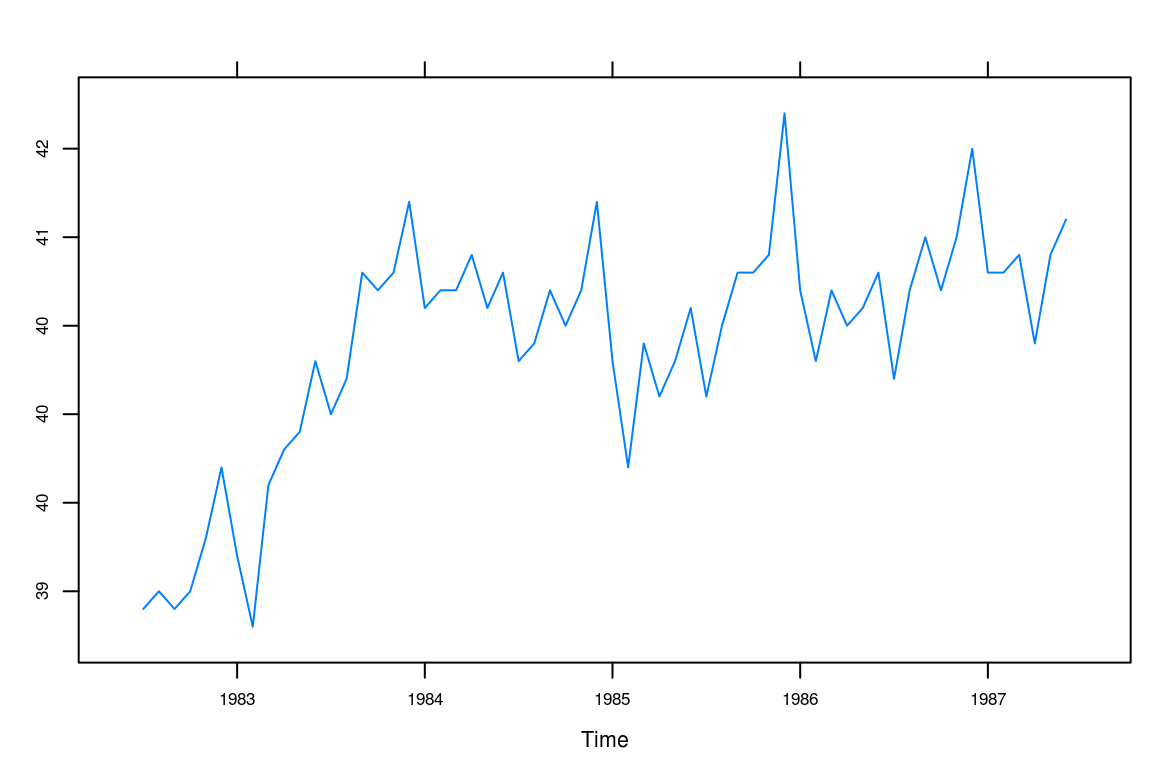
\includegraphics{TSAsolutions_files/figure-latex/unnamed-chunk-10-1.pdf}
\caption{\label{fig:unnamed-chunk-10}Monthly values of the average hours
worked per week in the U.S. manufacturing sector.}
\end{figure}

In Figure 1 we see a steep incline between 83 and 84. There also appears
to be a seasonal trend with generally longer work hours later in the
year apart from the summer; 1984, however, does not exhibit as clear a
pattern.

\subsection*{b}\label{b-21}
\addcontentsline{toc}{subsection}{b}

\begin{Shaded}
\begin{Highlighting}[]
\NormalTok{months <-}\StringTok{ }\KeywordTok{c}\NormalTok{(}\StringTok{"J"}\NormalTok{, }\StringTok{"A"}\NormalTok{, }\StringTok{"S"}\NormalTok{, }\StringTok{"O"}\NormalTok{, }\StringTok{"N"}\NormalTok{, }\StringTok{"D"}\NormalTok{, }\StringTok{"J"}\NormalTok{, }\StringTok{"F"}\NormalTok{, }\StringTok{"M"}\NormalTok{, }\StringTok{"A"}\NormalTok{, }\StringTok{"M"}\NormalTok{, }\StringTok{"J"}\NormalTok{)}

\KeywordTok{xyplot}\NormalTok{(hours, }\DataTypeTok{panel =} \NormalTok{function(x, y, ...) \{}
  \KeywordTok{panel.xyplot}\NormalTok{(x, y, ...)}
  \KeywordTok{panel.text}\NormalTok{(}\DataTypeTok{x =} \NormalTok{x, }\DataTypeTok{y =} \NormalTok{y, }\DataTypeTok{labels =} \NormalTok{months)}
\NormalTok{\})}
\end{Highlighting}
\end{Shaded}

\begin{figure}[htbp]
\centering
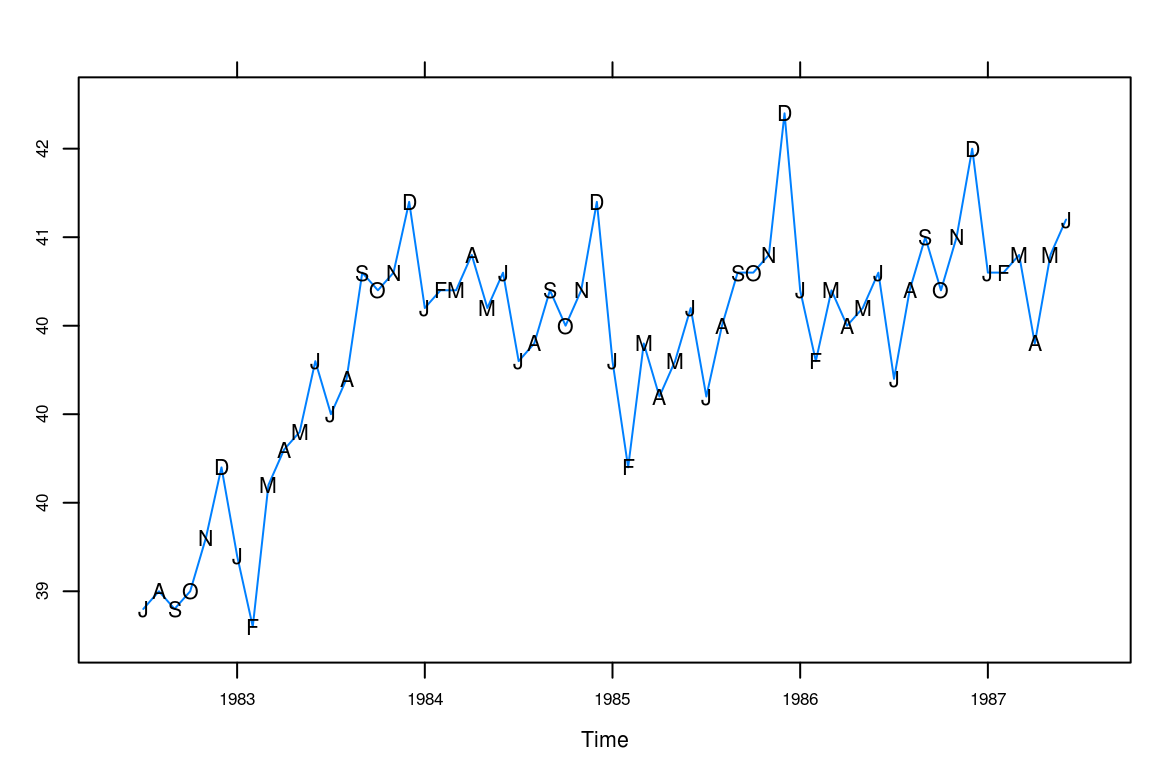
\includegraphics{TSAsolutions_files/figure-latex/unnamed-chunk-11-1.pdf}
\caption{\label{fig:unnamed-chunk-11}Monthly values of average hours worked
per week with superposed initials of months.}
\end{figure}

Here, in Figure 2, our interpretation is largely the same. It is clear
that December stands out as the month with the longest weekly work hours
whilst February and January are low-points, demonstrating a clear trend.

\section{Wages}\label{wages}

\subsection*{a}\label{a-22}
\addcontentsline{toc}{subsection}{a}

\begin{Shaded}
\begin{Highlighting}[]
\KeywordTok{data}\NormalTok{(}\StringTok{"wages"}\NormalTok{)}
\KeywordTok{xyplot}\NormalTok{(wages, }\DataTypeTok{panel =} \NormalTok{function(x, y, ...) \{}
  \KeywordTok{panel.xyplot}\NormalTok{(x, y, ...)}
  \KeywordTok{panel.text}\NormalTok{(x, y, }\DataTypeTok{labels =} \NormalTok{months)}
\NormalTok{\})}
\end{Highlighting}
\end{Shaded}

\begin{figure}[htbp]
\centering
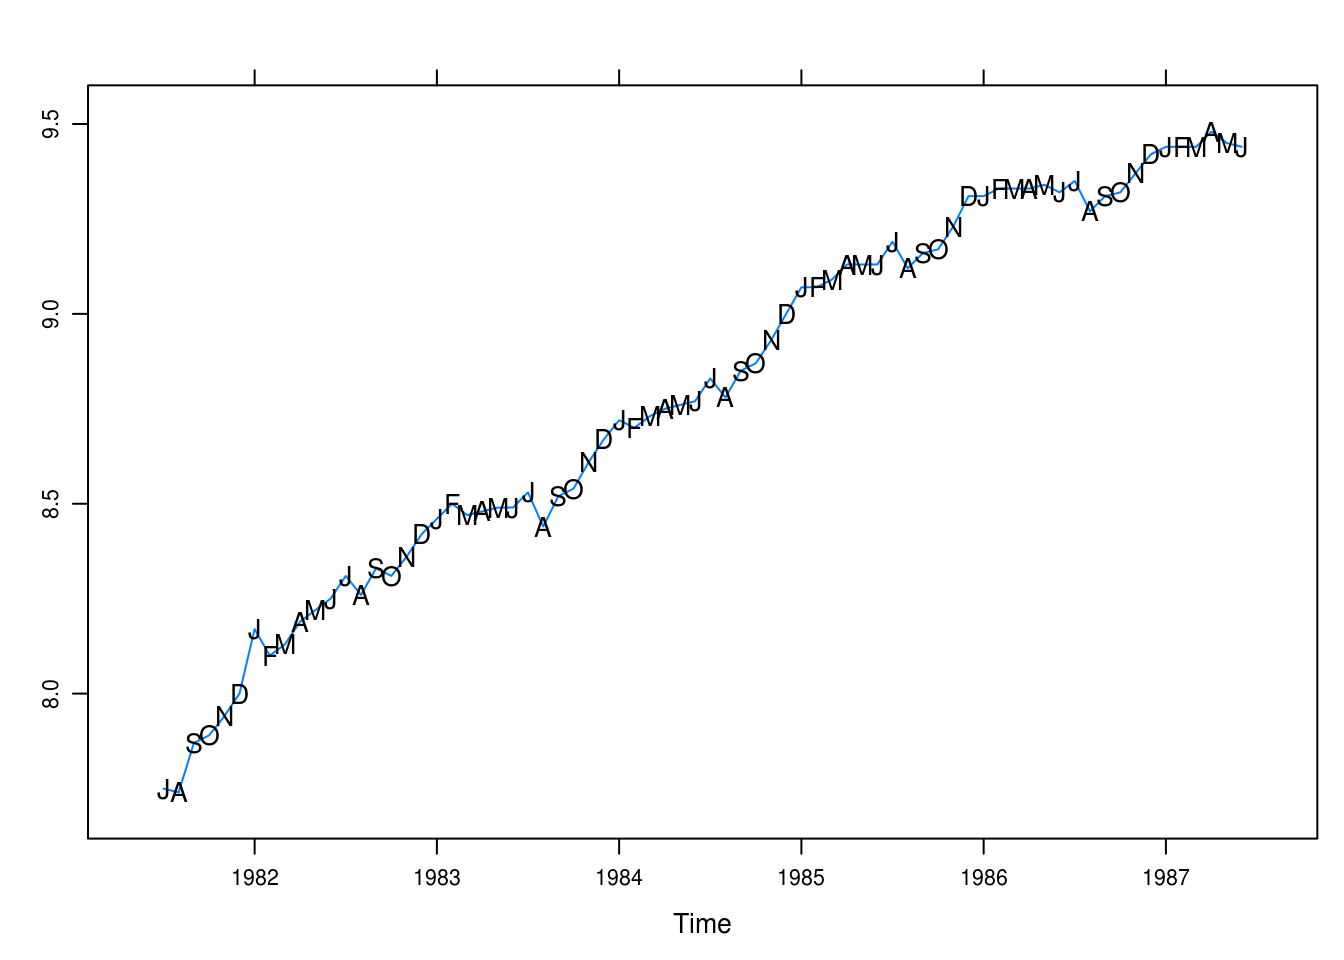
\includegraphics{TSAsolutions_files/figure-latex/unnamed-chunk-12-1.pdf}
\caption{\label{fig:unnamed-chunk-12}Monthly average hourly wages for
workers in the U.S. apparel and textile industry.}
\end{figure}

There is a positive trend with seasonality: August is a low-point for
wages. Generally, there seems to be larger increases in the fall.

\subsection*{b}\label{b-22}
\addcontentsline{toc}{subsection}{b}

\begin{Shaded}
\begin{Highlighting}[]
\NormalTok{wages_fit1 <-}\StringTok{ }\KeywordTok{lm}\NormalTok{(wages ~}\StringTok{ }\KeywordTok{time}\NormalTok{(wages))}
\KeywordTok{summary}\NormalTok{(wages_fit1)}
\end{Highlighting}
\end{Shaded}

\begin{verbatim}
## 
## Call:
## lm(formula = wages ~ time(wages))
## 
## Residuals:
##     Min      1Q  Median      3Q     Max 
## -0.2383 -0.0498  0.0194  0.0585  0.1314 
## 
## Coefficients:
##              Estimate Std. Error t value Pr(>|t|)    
## (Intercept) -5.49e+02   1.11e+01   -49.2   <2e-16 ***
## time(wages)  2.81e-01   5.62e-03    50.0   <2e-16 ***
## ---
## Signif. codes:  0 '***' 0.001 '**' 0.01 '*' 0.05 '.' 0.1 ' ' 1
## 
## Residual standard error: 0.083 on 70 degrees of freedom
## Multiple R-squared:  0.973,  Adjusted R-squared:  0.972 
## F-statistic: 2.5e+03 on 1 and 70 DF,  p-value: <2e-16
\end{verbatim}

\begin{Shaded}
\begin{Highlighting}[]
\NormalTok{wages_rst <-}\StringTok{ }\KeywordTok{rstudent}\NormalTok{(wages_fit1)}
\end{Highlighting}
\end{Shaded}

\subsection*{c}\label{c-11}
\addcontentsline{toc}{subsection}{c}

\begin{Shaded}
\begin{Highlighting}[]
\KeywordTok{xyplot}\NormalTok{(wages_rst ~}\StringTok{ }\KeywordTok{time}\NormalTok{(wages_rst), }\DataTypeTok{type =} \StringTok{"l"}\NormalTok{,}
       \DataTypeTok{xlab =} \StringTok{"Time"}\NormalTok{, }\DataTypeTok{ylab =} \StringTok{"Studentized residuals"}\NormalTok{)}
\end{Highlighting}
\end{Shaded}

\begin{figure}[htbp]
\centering
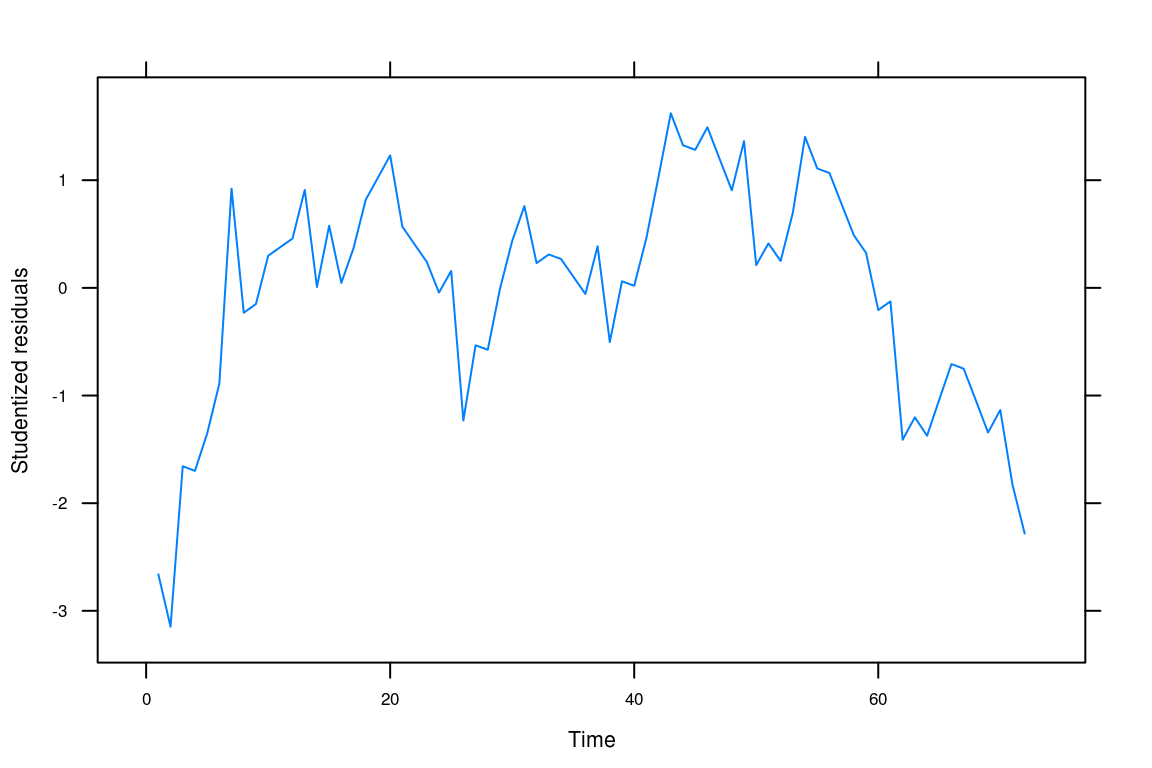
\includegraphics{TSAsolutions_files/figure-latex/wages_resid-1.pdf}
\caption{(\#fig:wages\_resid)Residual plot}
\end{figure}

We still seem to have autocorrelation related to the time and not white
noise.

\subsection*{d}\label{d-2}
\addcontentsline{toc}{subsection}{d}

\begin{Shaded}
\begin{Highlighting}[]
\NormalTok{wages_fit2 <-}\StringTok{ }\KeywordTok{lm}\NormalTok{(wages ~}\StringTok{ }\KeywordTok{time}\NormalTok{(wages) +}\StringTok{ }\KeywordTok{I}\NormalTok{(}\KeywordTok{time}\NormalTok{(wages)^}\DecValTok{2}\NormalTok{))}
\KeywordTok{summary}\NormalTok{(wages_fit2)}
\end{Highlighting}
\end{Shaded}

\begin{verbatim}
## 
## Call:
## lm(formula = wages ~ time(wages) + I(time(wages)^2))
## 
## Residuals:
##      Min       1Q   Median       3Q      Max 
## -0.14832 -0.04144  0.00156  0.05009  0.13984 
## 
## Coefficients:
##                   Estimate Std. Error t value Pr(>|t|)    
## (Intercept)      -8.49e+04   1.02e+04   -8.34  4.9e-12 ***
## time(wages)       8.53e+01   1.03e+01    8.31  5.4e-12 ***
## I(time(wages)^2) -2.14e-02   2.59e-03   -8.28  6.1e-12 ***
## ---
## Signif. codes:  0 '***' 0.001 '**' 0.01 '*' 0.05 '.' 0.1 ' ' 1
## 
## Residual standard error: 0.059 on 69 degrees of freedom
## Multiple R-squared:  0.986,  Adjusted R-squared:  0.986 
## F-statistic: 2.49e+03 on 2 and 69 DF,  p-value: <2e-16
\end{verbatim}

\begin{Shaded}
\begin{Highlighting}[]
\NormalTok{wages_rst2 <-}\StringTok{ }\KeywordTok{rstudent}\NormalTok{(wages_fit2)}
\end{Highlighting}
\end{Shaded}

\subsection*{e}\label{e-1}
\addcontentsline{toc}{subsection}{e}

\begin{Shaded}
\begin{Highlighting}[]
\KeywordTok{xyplot}\NormalTok{(wages_rst2 ~}\StringTok{ }\KeywordTok{time}\NormalTok{(wages_rst), }\DataTypeTok{type =} \StringTok{"l"}\NormalTok{,}
       \DataTypeTok{xlab =} \StringTok{"Time"}\NormalTok{, }\DataTypeTok{ylab =} \StringTok{"Studentized residuals"}\NormalTok{)}
\end{Highlighting}
\end{Shaded}

\begin{figure}[htbp]
\centering
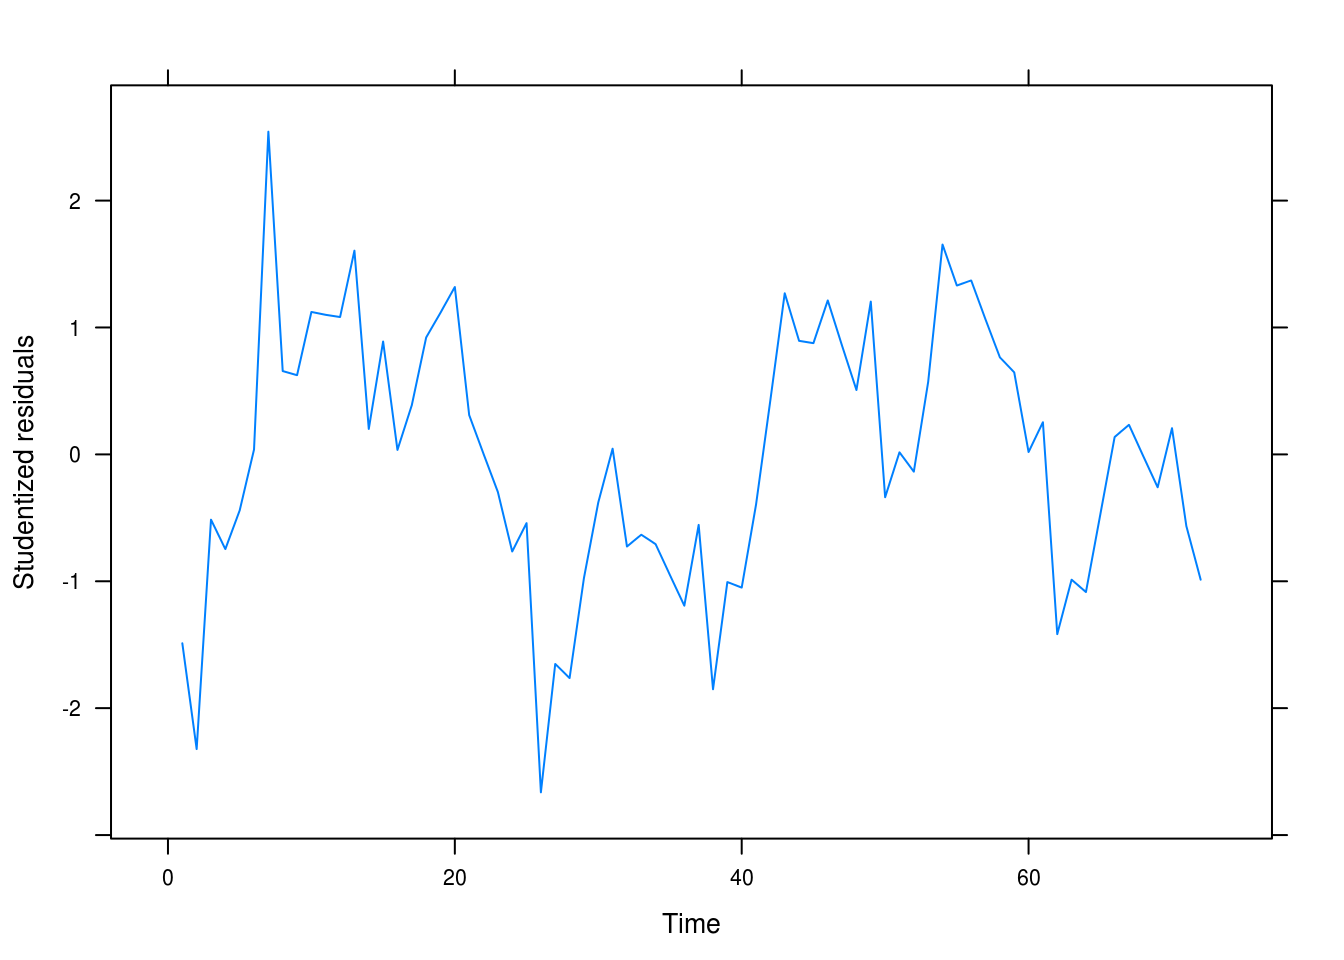
\includegraphics{TSAsolutions_files/figure-latex/wages_quad_resid-1.pdf}
\caption{(\#fig:wages\_quad\_resid)Residual plot for our quadratic
model.}
\end{figure}

This looks more like random noise but there is still clear
autocorrelation between the fitted residuals that we have yet to capture
in our model.

\section{Beer sales}\label{beer-sales}

\subsection*{a}\label{a-23}
\addcontentsline{toc}{subsection}{a}

\begin{Shaded}
\begin{Highlighting}[]
\KeywordTok{data}\NormalTok{(beersales)}
\KeywordTok{xyplot}\NormalTok{(beersales)}
\end{Highlighting}
\end{Shaded}

\begin{figure}[htbp]
\centering
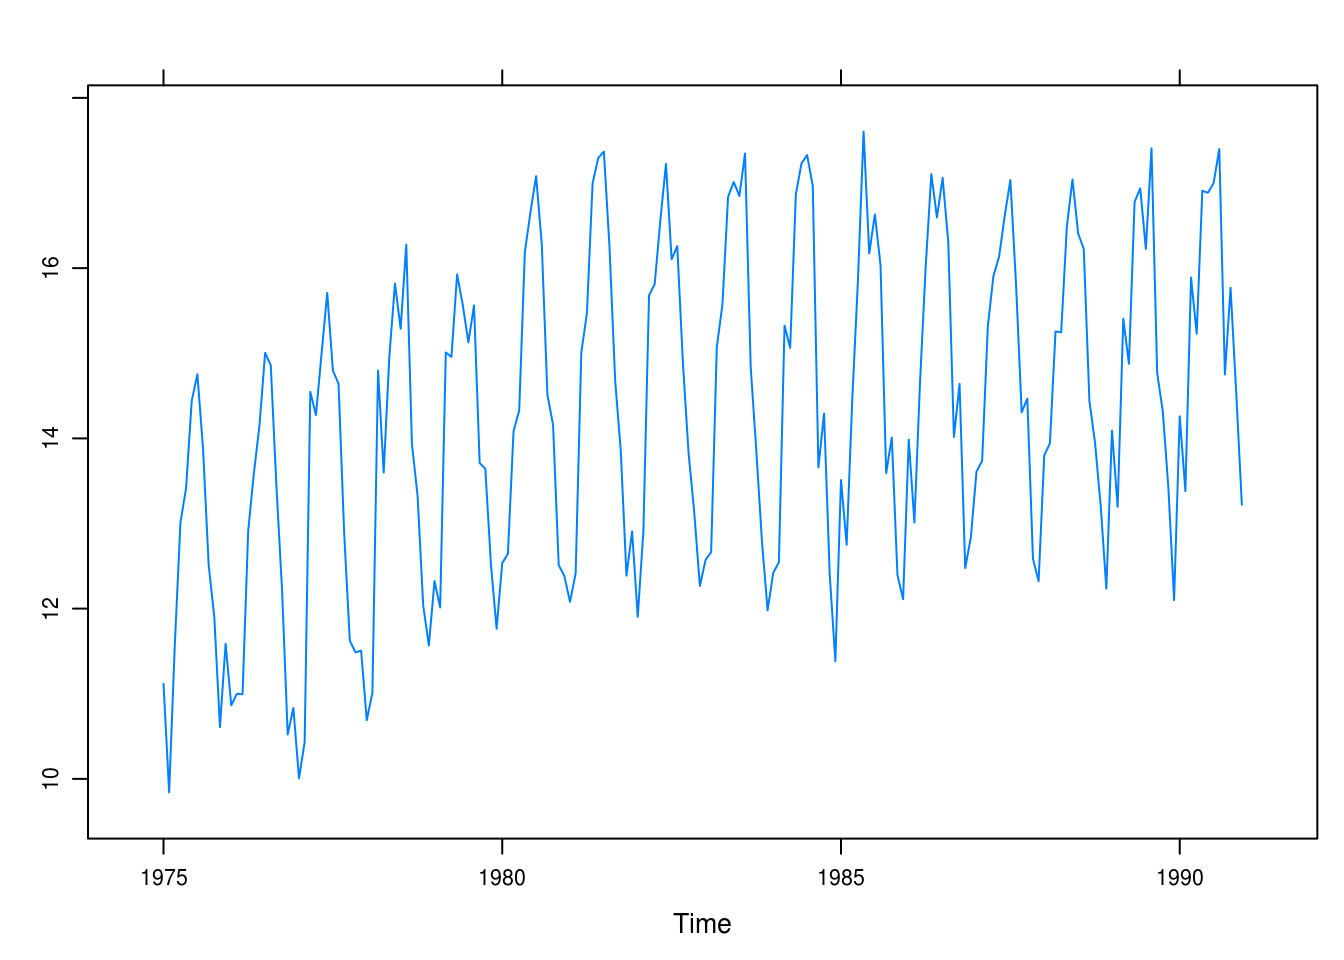
\includegraphics{TSAsolutions_files/figure-latex/unnamed-chunk-15-1.pdf}
\caption{\label{fig:unnamed-chunk-15}Monthly U.S. beer sales.}
\end{figure}

Clear seasonal trends. There is an initial positive trend from 1975 to
around 1981 that then levels out.

\subsection*{b}\label{b-23}
\addcontentsline{toc}{subsection}{b}

\begin{Shaded}
\begin{Highlighting}[]
\NormalTok{months <-}\StringTok{ }\KeywordTok{c}\NormalTok{(}\StringTok{"J"}\NormalTok{, }\StringTok{"F"}\NormalTok{, }\StringTok{"M"}\NormalTok{, }\StringTok{"A"}\NormalTok{, }\StringTok{"M"}\NormalTok{, }\StringTok{"J"}\NormalTok{, }\StringTok{"J"}\NormalTok{, }\StringTok{"A"}\NormalTok{, }\StringTok{"S"}\NormalTok{, }\StringTok{"O"}\NormalTok{, }\StringTok{"N"}\NormalTok{, }\StringTok{"D"}\NormalTok{)}

\KeywordTok{xyplot}\NormalTok{(beersales,}
       \DataTypeTok{panel =} \NormalTok{function(x, y, ...) \{}
         \KeywordTok{panel.xyplot}\NormalTok{(x, y, ...)}
         \KeywordTok{panel.text}\NormalTok{(x, y, }\DataTypeTok{labels =} \NormalTok{months)}
       \NormalTok{\})}
\end{Highlighting}
\end{Shaded}

\begin{figure}[htbp]
\centering
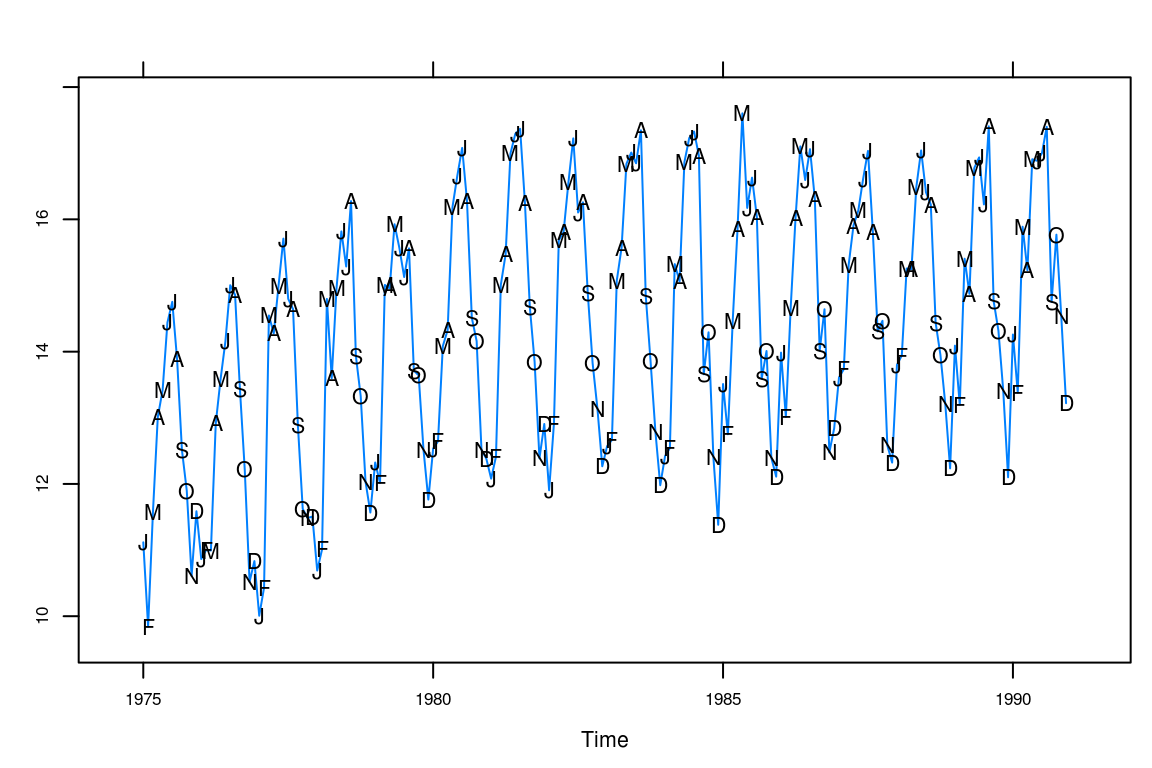
\includegraphics{TSAsolutions_files/figure-latex/unnamed-chunk-16-1.pdf}
\caption{\label{fig:unnamed-chunk-16}Monthly U.S. beer sales annotated with
the months' initials.}
\end{figure}

It is now evident that the peaks are in the warm months and the slump in
the winter and fall months. December is a particular low point, while
May, June, and July seem to be the high points.

\subsection*{c}\label{c-12}
\addcontentsline{toc}{subsection}{c}

\begin{Shaded}
\begin{Highlighting}[]
\NormalTok{beer_fit1 <-}\StringTok{ }\KeywordTok{lm}\NormalTok{(beersales ~}\StringTok{ }\KeywordTok{season}\NormalTok{(beersales))}
\KeywordTok{pander}\NormalTok{(}\KeywordTok{summary}\NormalTok{(beer_fit1))}
\end{Highlighting}
\end{Shaded}

\begin{longtable}[c]{@{}ccccc@{}}
\toprule
\begin{minipage}[b]{0.37\columnwidth}\centering\strut
~
\strut\end{minipage} &
\begin{minipage}[b]{0.12\columnwidth}\centering\strut
Estimate
\strut\end{minipage} &
\begin{minipage}[b]{0.14\columnwidth}\centering\strut
Std. Error
\strut\end{minipage} &
\begin{minipage}[b]{0.11\columnwidth}\centering\strut
t value
\strut\end{minipage} &
\begin{minipage}[b]{0.11\columnwidth}\centering\strut
Pr(\textgreater{}\textbar{}t\textbar{})
\strut\end{minipage}\tabularnewline
\midrule
\endhead
\begin{minipage}[t]{0.37\columnwidth}\centering\strut
\textbf{season(beersales)February}
\strut\end{minipage} &
\begin{minipage}[t]{0.12\columnwidth}\centering\strut
-0.1426
\strut\end{minipage} &
\begin{minipage}[t]{0.14\columnwidth}\centering\strut
0.3732
\strut\end{minipage} &
\begin{minipage}[t]{0.11\columnwidth}\centering\strut
-0.382
\strut\end{minipage} &
\begin{minipage}[t]{0.11\columnwidth}\centering\strut
0.7029
\strut\end{minipage}\tabularnewline
\begin{minipage}[t]{0.37\columnwidth}\centering\strut
\textbf{season(beersales)March}
\strut\end{minipage} &
\begin{minipage}[t]{0.12\columnwidth}\centering\strut
2.082
\strut\end{minipage} &
\begin{minipage}[t]{0.14\columnwidth}\centering\strut
0.3732
\strut\end{minipage} &
\begin{minipage}[t]{0.11\columnwidth}\centering\strut
5.579
\strut\end{minipage} &
\begin{minipage}[t]{0.11\columnwidth}\centering\strut
8.771e-08
\strut\end{minipage}\tabularnewline
\begin{minipage}[t]{0.37\columnwidth}\centering\strut
\textbf{season(beersales)April}
\strut\end{minipage} &
\begin{minipage}[t]{0.12\columnwidth}\centering\strut
2.398
\strut\end{minipage} &
\begin{minipage}[t]{0.14\columnwidth}\centering\strut
0.3732
\strut\end{minipage} &
\begin{minipage}[t]{0.11\columnwidth}\centering\strut
6.424
\strut\end{minipage} &
\begin{minipage}[t]{0.11\columnwidth}\centering\strut
1.151e-09
\strut\end{minipage}\tabularnewline
\begin{minipage}[t]{0.37\columnwidth}\centering\strut
\textbf{season(beersales)May}
\strut\end{minipage} &
\begin{minipage}[t]{0.12\columnwidth}\centering\strut
3.599
\strut\end{minipage} &
\begin{minipage}[t]{0.14\columnwidth}\centering\strut
0.3732
\strut\end{minipage} &
\begin{minipage}[t]{0.11\columnwidth}\centering\strut
9.643
\strut\end{minipage} &
\begin{minipage}[t]{0.11\columnwidth}\centering\strut
5.322e-18
\strut\end{minipage}\tabularnewline
\begin{minipage}[t]{0.37\columnwidth}\centering\strut
\textbf{season(beersales)June}
\strut\end{minipage} &
\begin{minipage}[t]{0.12\columnwidth}\centering\strut
3.85
\strut\end{minipage} &
\begin{minipage}[t]{0.14\columnwidth}\centering\strut
0.3732
\strut\end{minipage} &
\begin{minipage}[t]{0.11\columnwidth}\centering\strut
10.31
\strut\end{minipage} &
\begin{minipage}[t]{0.11\columnwidth}\centering\strut
6.813e-20
\strut\end{minipage}\tabularnewline
\begin{minipage}[t]{0.37\columnwidth}\centering\strut
\textbf{season(beersales)July}
\strut\end{minipage} &
\begin{minipage}[t]{0.12\columnwidth}\centering\strut
3.769
\strut\end{minipage} &
\begin{minipage}[t]{0.14\columnwidth}\centering\strut
0.3732
\strut\end{minipage} &
\begin{minipage}[t]{0.11\columnwidth}\centering\strut
10.1
\strut\end{minipage} &
\begin{minipage}[t]{0.11\columnwidth}\centering\strut
2.812e-19
\strut\end{minipage}\tabularnewline
\begin{minipage}[t]{0.37\columnwidth}\centering\strut
\textbf{season(beersales)August}
\strut\end{minipage} &
\begin{minipage}[t]{0.12\columnwidth}\centering\strut
3.609
\strut\end{minipage} &
\begin{minipage}[t]{0.14\columnwidth}\centering\strut
0.3732
\strut\end{minipage} &
\begin{minipage}[t]{0.11\columnwidth}\centering\strut
9.669
\strut\end{minipage} &
\begin{minipage}[t]{0.11\columnwidth}\centering\strut
4.494e-18
\strut\end{minipage}\tabularnewline
\begin{minipage}[t]{0.37\columnwidth}\centering\strut
\textbf{season(beersales)September}
\strut\end{minipage} &
\begin{minipage}[t]{0.12\columnwidth}\centering\strut
1.573
\strut\end{minipage} &
\begin{minipage}[t]{0.14\columnwidth}\centering\strut
0.3732
\strut\end{minipage} &
\begin{minipage}[t]{0.11\columnwidth}\centering\strut
4.214
\strut\end{minipage} &
\begin{minipage}[t]{0.11\columnwidth}\centering\strut
3.964e-05
\strut\end{minipage}\tabularnewline
\begin{minipage}[t]{0.37\columnwidth}\centering\strut
\textbf{season(beersales)October}
\strut\end{minipage} &
\begin{minipage}[t]{0.12\columnwidth}\centering\strut
1.254
\strut\end{minipage} &
\begin{minipage}[t]{0.14\columnwidth}\centering\strut
0.3732
\strut\end{minipage} &
\begin{minipage}[t]{0.11\columnwidth}\centering\strut
3.361
\strut\end{minipage} &
\begin{minipage}[t]{0.11\columnwidth}\centering\strut
0.0009484
\strut\end{minipage}\tabularnewline
\begin{minipage}[t]{0.37\columnwidth}\centering\strut
\textbf{season(beersales)November}
\strut\end{minipage} &
\begin{minipage}[t]{0.12\columnwidth}\centering\strut
-0.04797
\strut\end{minipage} &
\begin{minipage}[t]{0.14\columnwidth}\centering\strut
0.3732
\strut\end{minipage} &
\begin{minipage}[t]{0.11\columnwidth}\centering\strut
-0.1285
\strut\end{minipage} &
\begin{minipage}[t]{0.11\columnwidth}\centering\strut
0.8979
\strut\end{minipage}\tabularnewline
\begin{minipage}[t]{0.37\columnwidth}\centering\strut
\textbf{season(beersales)December}
\strut\end{minipage} &
\begin{minipage}[t]{0.12\columnwidth}\centering\strut
-0.4231
\strut\end{minipage} &
\begin{minipage}[t]{0.14\columnwidth}\centering\strut
0.3732
\strut\end{minipage} &
\begin{minipage}[t]{0.11\columnwidth}\centering\strut
-1.134
\strut\end{minipage} &
\begin{minipage}[t]{0.11\columnwidth}\centering\strut
0.2585
\strut\end{minipage}\tabularnewline
\begin{minipage}[t]{0.37\columnwidth}\centering\strut
\textbf{(Intercept)}
\strut\end{minipage} &
\begin{minipage}[t]{0.12\columnwidth}\centering\strut
12.49
\strut\end{minipage} &
\begin{minipage}[t]{0.14\columnwidth}\centering\strut
0.2639
\strut\end{minipage} &
\begin{minipage}[t]{0.11\columnwidth}\centering\strut
47.31
\strut\end{minipage} &
\begin{minipage}[t]{0.11\columnwidth}\centering\strut
1.786e-103
\strut\end{minipage}\tabularnewline
\bottomrule
\end{longtable}

\begin{longtable}[c]{@{}cccc@{}}
\caption{Fitting linear model: beersales \textasciitilde{}
season(beersales)}\tabularnewline
\toprule
\begin{minipage}[b]{0.18\columnwidth}\centering\strut
Observations
\strut\end{minipage} &
\begin{minipage}[b]{0.27\columnwidth}\centering\strut
Residual Std. Error
\strut\end{minipage} &
\begin{minipage}[b]{0.10\columnwidth}\centering\strut
\(R^2\)
\strut\end{minipage} &
\begin{minipage}[b]{0.20\columnwidth}\centering\strut
Adjusted \(R^2\)
\strut\end{minipage}\tabularnewline
\midrule
\endfirsthead
\toprule
\begin{minipage}[b]{0.18\columnwidth}\centering\strut
Observations
\strut\end{minipage} &
\begin{minipage}[b]{0.27\columnwidth}\centering\strut
Residual Std. Error
\strut\end{minipage} &
\begin{minipage}[b]{0.10\columnwidth}\centering\strut
\(R^2\)
\strut\end{minipage} &
\begin{minipage}[b]{0.20\columnwidth}\centering\strut
Adjusted \(R^2\)
\strut\end{minipage}\tabularnewline
\midrule
\endhead
\begin{minipage}[t]{0.18\columnwidth}\centering\strut
192
\strut\end{minipage} &
\begin{minipage}[t]{0.27\columnwidth}\centering\strut
1.056
\strut\end{minipage} &
\begin{minipage}[t]{0.10\columnwidth}\centering\strut
0.7103
\strut\end{minipage} &
\begin{minipage}[t]{0.20\columnwidth}\centering\strut
0.6926
\strut\end{minipage}\tabularnewline
\bottomrule
\end{longtable}

All comparisons are made against january. The model helpfully explains
approximately 0.71 of the variance and is statistically significant.
Most of the factors are significant (mostly the winter months as
expected).

\subsection*{d}\label{d-3}
\addcontentsline{toc}{subsection}{d}

\begin{Shaded}
\begin{Highlighting}[]
\KeywordTok{xyplot}\NormalTok{(}\KeywordTok{rstudent}\NormalTok{(beer_fit1) ~}\StringTok{ }\KeywordTok{time}\NormalTok{(beersales), }\DataTypeTok{type =} \StringTok{"l"}\NormalTok{,}
       \DataTypeTok{xlab =} \StringTok{"Time"}\NormalTok{, }\DataTypeTok{ylab =} \StringTok{"Studentized residuals"}\NormalTok{,}
       \DataTypeTok{panel =} \NormalTok{function(x, y, ...) \{}
         \KeywordTok{panel.xyplot}\NormalTok{(x, y, ...)}
         \KeywordTok{panel.xyplot}\NormalTok{(x, y, }\DataTypeTok{pch =} \KeywordTok{as.vector}\NormalTok{(}\KeywordTok{season}\NormalTok{(beersales)), }\DataTypeTok{col =} \DecValTok{1}\NormalTok{)}
       \NormalTok{\})}
\end{Highlighting}
\end{Shaded}

\begin{figure}[htbp]
\centering
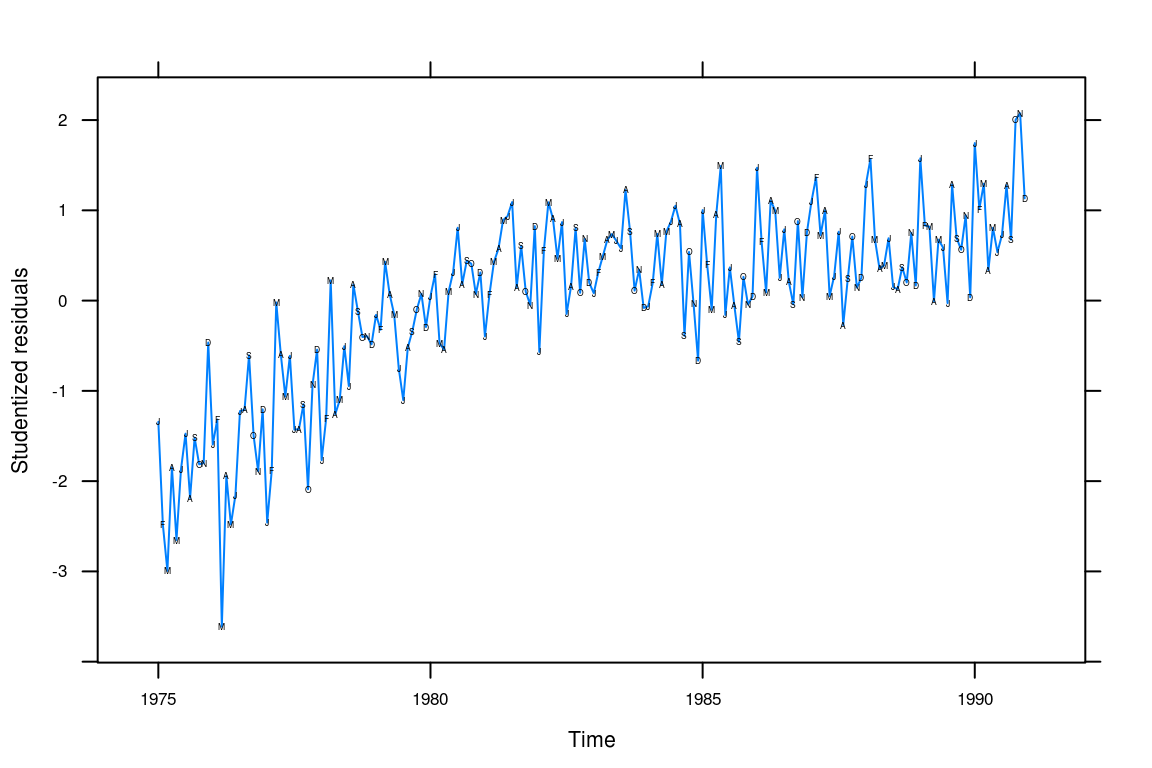
\includegraphics{TSAsolutions_files/figure-latex/rst-beer-1.pdf}
\caption{\label{fig:rst-beer}Beer sales residual plot.}
\end{figure}

Looking at the residuals in \ref{fig:rst-beer} We don't have a good fit
to our data; in particular, wee're not capturing the long-term trend.

\subsection*{e}\label{e-2}
\addcontentsline{toc}{subsection}{e}

\begin{Shaded}
\begin{Highlighting}[]
\NormalTok{beer_fit2 <-}\StringTok{ }\KeywordTok{lm}\NormalTok{(beersales ~}\StringTok{ }\KeywordTok{season}\NormalTok{(beersales) +}\StringTok{ }\KeywordTok{time}\NormalTok{(beersales) +}
\StringTok{                  }\KeywordTok{I}\NormalTok{(}\KeywordTok{time}\NormalTok{(beersales) ^}\StringTok{ }\DecValTok{2}\NormalTok{))}
\KeywordTok{pander}\NormalTok{(}\KeywordTok{summary}\NormalTok{(beer_fit2))}
\end{Highlighting}
\end{Shaded}

\begin{longtable}[c]{@{}ccccc@{}}
\toprule
\begin{minipage}[b]{0.37\columnwidth}\centering\strut
~
\strut\end{minipage} &
\begin{minipage}[b]{0.12\columnwidth}\centering\strut
Estimate
\strut\end{minipage} &
\begin{minipage}[b]{0.14\columnwidth}\centering\strut
Std. Error
\strut\end{minipage} &
\begin{minipage}[b]{0.11\columnwidth}\centering\strut
t value
\strut\end{minipage} &
\begin{minipage}[b]{0.11\columnwidth}\centering\strut
Pr(\textgreater{}\textbar{}t\textbar{})
\strut\end{minipage}\tabularnewline
\midrule
\endhead
\begin{minipage}[t]{0.37\columnwidth}\centering\strut
\textbf{season(beersales)February}
\strut\end{minipage} &
\begin{minipage}[t]{0.12\columnwidth}\centering\strut
-0.1579
\strut\end{minipage} &
\begin{minipage}[t]{0.14\columnwidth}\centering\strut
0.209
\strut\end{minipage} &
\begin{minipage}[t]{0.11\columnwidth}\centering\strut
-0.7554
\strut\end{minipage} &
\begin{minipage}[t]{0.11\columnwidth}\centering\strut
0.451
\strut\end{minipage}\tabularnewline
\begin{minipage}[t]{0.37\columnwidth}\centering\strut
\textbf{season(beersales)March}
\strut\end{minipage} &
\begin{minipage}[t]{0.12\columnwidth}\centering\strut
2.052
\strut\end{minipage} &
\begin{minipage}[t]{0.14\columnwidth}\centering\strut
0.209
\strut\end{minipage} &
\begin{minipage}[t]{0.11\columnwidth}\centering\strut
9.818
\strut\end{minipage} &
\begin{minipage}[t]{0.11\columnwidth}\centering\strut
1.864e-18
\strut\end{minipage}\tabularnewline
\begin{minipage}[t]{0.37\columnwidth}\centering\strut
\textbf{season(beersales)April}
\strut\end{minipage} &
\begin{minipage}[t]{0.12\columnwidth}\centering\strut
2.353
\strut\end{minipage} &
\begin{minipage}[t]{0.14\columnwidth}\centering\strut
0.209
\strut\end{minipage} &
\begin{minipage}[t]{0.11\columnwidth}\centering\strut
11.26
\strut\end{minipage} &
\begin{minipage}[t]{0.11\columnwidth}\centering\strut
1.533e-22
\strut\end{minipage}\tabularnewline
\begin{minipage}[t]{0.37\columnwidth}\centering\strut
\textbf{season(beersales)May}
\strut\end{minipage} &
\begin{minipage}[t]{0.12\columnwidth}\centering\strut
3.539
\strut\end{minipage} &
\begin{minipage}[t]{0.14\columnwidth}\centering\strut
0.209
\strut\end{minipage} &
\begin{minipage}[t]{0.11\columnwidth}\centering\strut
16.93
\strut\end{minipage} &
\begin{minipage}[t]{0.11\columnwidth}\centering\strut
6.063e-39
\strut\end{minipage}\tabularnewline
\begin{minipage}[t]{0.37\columnwidth}\centering\strut
\textbf{season(beersales)June}
\strut\end{minipage} &
\begin{minipage}[t]{0.12\columnwidth}\centering\strut
3.776
\strut\end{minipage} &
\begin{minipage}[t]{0.14\columnwidth}\centering\strut
0.209
\strut\end{minipage} &
\begin{minipage}[t]{0.11\columnwidth}\centering\strut
18.06
\strut\end{minipage} &
\begin{minipage}[t]{0.11\columnwidth}\centering\strut
4.117e-42
\strut\end{minipage}\tabularnewline
\begin{minipage}[t]{0.37\columnwidth}\centering\strut
\textbf{season(beersales)July}
\strut\end{minipage} &
\begin{minipage}[t]{0.12\columnwidth}\centering\strut
3.681
\strut\end{minipage} &
\begin{minipage}[t]{0.14\columnwidth}\centering\strut
0.209
\strut\end{minipage} &
\begin{minipage}[t]{0.11\columnwidth}\centering\strut
17.61
\strut\end{minipage} &
\begin{minipage}[t]{0.11\columnwidth}\centering\strut
7.706e-41
\strut\end{minipage}\tabularnewline
\begin{minipage}[t]{0.37\columnwidth}\centering\strut
\textbf{season(beersales)August}
\strut\end{minipage} &
\begin{minipage}[t]{0.12\columnwidth}\centering\strut
3.507
\strut\end{minipage} &
\begin{minipage}[t]{0.14\columnwidth}\centering\strut
0.2091
\strut\end{minipage} &
\begin{minipage}[t]{0.11\columnwidth}\centering\strut
16.78
\strut\end{minipage} &
\begin{minipage}[t]{0.11\columnwidth}\centering\strut
1.698e-38
\strut\end{minipage}\tabularnewline
\begin{minipage}[t]{0.37\columnwidth}\centering\strut
\textbf{season(beersales)September}
\strut\end{minipage} &
\begin{minipage}[t]{0.12\columnwidth}\centering\strut
1.458
\strut\end{minipage} &
\begin{minipage}[t]{0.14\columnwidth}\centering\strut
0.2091
\strut\end{minipage} &
\begin{minipage}[t]{0.11\columnwidth}\centering\strut
6.972
\strut\end{minipage} &
\begin{minipage}[t]{0.11\columnwidth}\centering\strut
5.89e-11
\strut\end{minipage}\tabularnewline
\begin{minipage}[t]{0.37\columnwidth}\centering\strut
\textbf{season(beersales)October}
\strut\end{minipage} &
\begin{minipage}[t]{0.12\columnwidth}\centering\strut
1.126
\strut\end{minipage} &
\begin{minipage}[t]{0.14\columnwidth}\centering\strut
0.2091
\strut\end{minipage} &
\begin{minipage}[t]{0.11\columnwidth}\centering\strut
5.385
\strut\end{minipage} &
\begin{minipage}[t]{0.11\columnwidth}\centering\strut
2.268e-07
\strut\end{minipage}\tabularnewline
\begin{minipage}[t]{0.37\columnwidth}\centering\strut
\textbf{season(beersales)November}
\strut\end{minipage} &
\begin{minipage}[t]{0.12\columnwidth}\centering\strut
-0.1894
\strut\end{minipage} &
\begin{minipage}[t]{0.14\columnwidth}\centering\strut
0.2091
\strut\end{minipage} &
\begin{minipage}[t]{0.11\columnwidth}\centering\strut
-0.9059
\strut\end{minipage} &
\begin{minipage}[t]{0.11\columnwidth}\centering\strut
0.3662
\strut\end{minipage}\tabularnewline
\begin{minipage}[t]{0.37\columnwidth}\centering\strut
\textbf{season(beersales)December}
\strut\end{minipage} &
\begin{minipage}[t]{0.12\columnwidth}\centering\strut
-0.5773
\strut\end{minipage} &
\begin{minipage}[t]{0.14\columnwidth}\centering\strut
0.2092
\strut\end{minipage} &
\begin{minipage}[t]{0.11\columnwidth}\centering\strut
-2.76
\strut\end{minipage} &
\begin{minipage}[t]{0.11\columnwidth}\centering\strut
0.00638
\strut\end{minipage}\tabularnewline
\begin{minipage}[t]{0.37\columnwidth}\centering\strut
\textbf{time(beersales)}
\strut\end{minipage} &
\begin{minipage}[t]{0.12\columnwidth}\centering\strut
71.96
\strut\end{minipage} &
\begin{minipage}[t]{0.14\columnwidth}\centering\strut
8.867
\strut\end{minipage} &
\begin{minipage}[t]{0.11\columnwidth}\centering\strut
8.115
\strut\end{minipage} &
\begin{minipage}[t]{0.11\columnwidth}\centering\strut
7.703e-14
\strut\end{minipage}\tabularnewline
\begin{minipage}[t]{0.37\columnwidth}\centering\strut
\textbf{I(time(beersales)\^{}2)}
\strut\end{minipage} &
\begin{minipage}[t]{0.12\columnwidth}\centering\strut
-0.0181
\strut\end{minipage} &
\begin{minipage}[t]{0.14\columnwidth}\centering\strut
0.002236
\strut\end{minipage} &
\begin{minipage}[t]{0.11\columnwidth}\centering\strut
-8.096
\strut\end{minipage} &
\begin{minipage}[t]{0.11\columnwidth}\centering\strut
8.633e-14
\strut\end{minipage}\tabularnewline
\begin{minipage}[t]{0.37\columnwidth}\centering\strut
\textbf{(Intercept)}
\strut\end{minipage} &
\begin{minipage}[t]{0.12\columnwidth}\centering\strut
-71498
\strut\end{minipage} &
\begin{minipage}[t]{0.14\columnwidth}\centering\strut
8791
\strut\end{minipage} &
\begin{minipage}[t]{0.11\columnwidth}\centering\strut
-8.133
\strut\end{minipage} &
\begin{minipage}[t]{0.11\columnwidth}\centering\strut
6.932e-14
\strut\end{minipage}\tabularnewline
\bottomrule
\end{longtable}

\begin{longtable}[c]{@{}cccc@{}}
\caption{Fitting linear model: beersales \textasciitilde{}
season(beersales) + time(beersales) +
I(time(beersales)\^{}2)}\tabularnewline
\toprule
\begin{minipage}[b]{0.18\columnwidth}\centering\strut
Observations
\strut\end{minipage} &
\begin{minipage}[b]{0.27\columnwidth}\centering\strut
Residual Std. Error
\strut\end{minipage} &
\begin{minipage}[b]{0.10\columnwidth}\centering\strut
\(R^2\)
\strut\end{minipage} &
\begin{minipage}[b]{0.20\columnwidth}\centering\strut
Adjusted \(R^2\)
\strut\end{minipage}\tabularnewline
\midrule
\endfirsthead
\toprule
\begin{minipage}[b]{0.18\columnwidth}\centering\strut
Observations
\strut\end{minipage} &
\begin{minipage}[b]{0.27\columnwidth}\centering\strut
Residual Std. Error
\strut\end{minipage} &
\begin{minipage}[b]{0.10\columnwidth}\centering\strut
\(R^2\)
\strut\end{minipage} &
\begin{minipage}[b]{0.20\columnwidth}\centering\strut
Adjusted \(R^2\)
\strut\end{minipage}\tabularnewline
\midrule
\endhead
\begin{minipage}[t]{0.18\columnwidth}\centering\strut
192
\strut\end{minipage} &
\begin{minipage}[t]{0.27\columnwidth}\centering\strut
0.5911
\strut\end{minipage} &
\begin{minipage}[t]{0.10\columnwidth}\centering\strut
0.9102
\strut\end{minipage} &
\begin{minipage}[t]{0.20\columnwidth}\centering\strut
0.9036
\strut\end{minipage}\tabularnewline
\bottomrule
\end{longtable}

This model fits the data better, explaining roughly 0.91 of the
variance.

\subsection*{f}\label{f}
\addcontentsline{toc}{subsection}{f}

\begin{Shaded}
\begin{Highlighting}[]
\KeywordTok{xyplot}\NormalTok{(}\KeywordTok{rstudent}\NormalTok{(beer_fit2) ~}\StringTok{ }\KeywordTok{time}\NormalTok{(beersales), }\DataTypeTok{type =} \StringTok{"l"}\NormalTok{,}
       \DataTypeTok{xlab =} \StringTok{"Time"}\NormalTok{, }\DataTypeTok{yla =} \StringTok{"Studentized residuals"}\NormalTok{,}
       \DataTypeTok{panel =} \NormalTok{function(x, y, ...) \{}
         \KeywordTok{panel.xyplot}\NormalTok{(x, y, ...)}
         \KeywordTok{panel.xyplot}\NormalTok{(x, y, }\DataTypeTok{pch =} \KeywordTok{as.vector}\NormalTok{(}\KeywordTok{season}\NormalTok{(beersales)), }\DataTypeTok{col =} \DecValTok{1}\NormalTok{)}
       \NormalTok{\})}
\end{Highlighting}
\end{Shaded}

\begin{figure}[htbp]
\centering
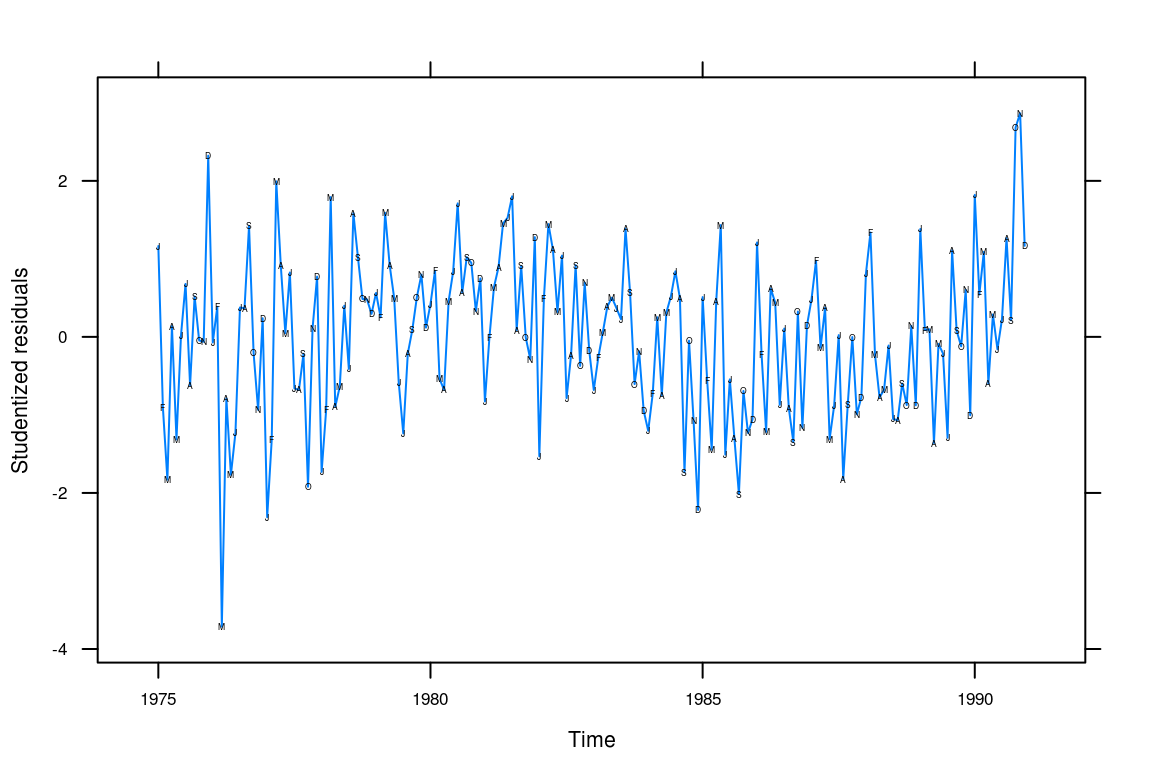
\includegraphics{TSAsolutions_files/figure-latex/rst-beer2-1.pdf}
\caption{\label{fig:rst-beer2}Beer sales residual plot from the quadratic
fit.}
\end{figure}

Many of the values are still not being predicted successfully but at
least we're able to model the long term trend better.

\section{Winnebago}\label{winnebago}

\subsection*{a}\label{a-24}
\addcontentsline{toc}{subsection}{a}

\begin{Shaded}
\begin{Highlighting}[]
\KeywordTok{data}\NormalTok{(winnebago)}
\KeywordTok{xyplot}\NormalTok{(winnebago)}
\end{Highlighting}
\end{Shaded}

\begin{figure}[htbp]
\centering
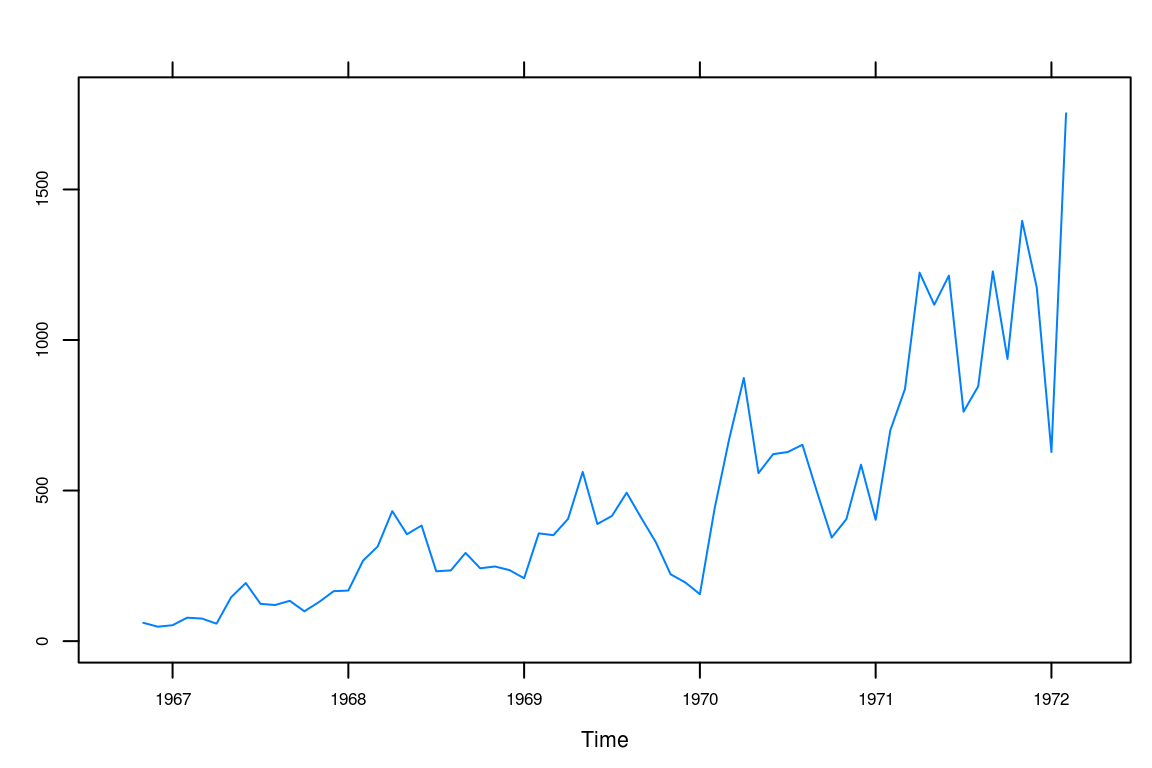
\includegraphics{TSAsolutions_files/figure-latex/unnamed-chunk-19-1.pdf}
\caption{\label{fig:unnamed-chunk-19}Monthly unit sales of recreational
vehicles from Winnebago.}
\end{figure}

\subsection*{b}\label{b-24}
\addcontentsline{toc}{subsection}{b}

\begin{Shaded}
\begin{Highlighting}[]
\NormalTok{winn_fit1 <-}\StringTok{ }\KeywordTok{lm}\NormalTok{(winnebago ~}\StringTok{ }\KeywordTok{time}\NormalTok{(winnebago))}
\KeywordTok{summary}\NormalTok{(winn_fit1) %>%}
\StringTok{  }\KeywordTok{pander}\NormalTok{()}
\end{Highlighting}
\end{Shaded}

\begin{longtable}[c]{@{}ccccc@{}}
\toprule
\begin{minipage}[b]{0.26\columnwidth}\centering\strut
~
\strut\end{minipage} &
\begin{minipage}[b]{0.13\columnwidth}\centering\strut
Estimate
\strut\end{minipage} &
\begin{minipage}[b]{0.16\columnwidth}\centering\strut
Std. Error
\strut\end{minipage} &
\begin{minipage}[b]{0.12\columnwidth}\centering\strut
t value
\strut\end{minipage} &
\begin{minipage}[b]{0.12\columnwidth}\centering\strut
Pr(\textgreater{}\textbar{}t\textbar{})
\strut\end{minipage}\tabularnewline
\midrule
\endhead
\begin{minipage}[t]{0.26\columnwidth}\centering\strut
\textbf{time(winnebago)}
\strut\end{minipage} &
\begin{minipage}[t]{0.13\columnwidth}\centering\strut
200.7
\strut\end{minipage} &
\begin{minipage}[t]{0.16\columnwidth}\centering\strut
17.03
\strut\end{minipage} &
\begin{minipage}[t]{0.12\columnwidth}\centering\strut
11.79
\strut\end{minipage} &
\begin{minipage}[t]{0.12\columnwidth}\centering\strut
1.777e-17
\strut\end{minipage}\tabularnewline
\begin{minipage}[t]{0.26\columnwidth}\centering\strut
\textbf{(Intercept)}
\strut\end{minipage} &
\begin{minipage}[t]{0.13\columnwidth}\centering\strut
-394886
\strut\end{minipage} &
\begin{minipage}[t]{0.16\columnwidth}\centering\strut
33540
\strut\end{minipage} &
\begin{minipage}[t]{0.12\columnwidth}\centering\strut
-11.77
\strut\end{minipage} &
\begin{minipage}[t]{0.12\columnwidth}\centering\strut
1.87e-17
\strut\end{minipage}\tabularnewline
\bottomrule
\end{longtable}

\begin{longtable}[c]{@{}cccc@{}}
\caption{Fitting linear model: winnebago \textasciitilde{}
time(winnebago)}\tabularnewline
\toprule
\begin{minipage}[b]{0.18\columnwidth}\centering\strut
Observations
\strut\end{minipage} &
\begin{minipage}[b]{0.27\columnwidth}\centering\strut
Residual Std. Error
\strut\end{minipage} &
\begin{minipage}[b]{0.10\columnwidth}\centering\strut
\(R^2\)
\strut\end{minipage} &
\begin{minipage}[b]{0.20\columnwidth}\centering\strut
Adjusted \(R^2\)
\strut\end{minipage}\tabularnewline
\midrule
\endfirsthead
\toprule
\begin{minipage}[b]{0.18\columnwidth}\centering\strut
Observations
\strut\end{minipage} &
\begin{minipage}[b]{0.27\columnwidth}\centering\strut
Residual Std. Error
\strut\end{minipage} &
\begin{minipage}[b]{0.10\columnwidth}\centering\strut
\(R^2\)
\strut\end{minipage} &
\begin{minipage}[b]{0.20\columnwidth}\centering\strut
Adjusted \(R^2\)
\strut\end{minipage}\tabularnewline
\midrule
\endhead
\begin{minipage}[t]{0.18\columnwidth}\centering\strut
64
\strut\end{minipage} &
\begin{minipage}[t]{0.27\columnwidth}\centering\strut
209.7
\strut\end{minipage} &
\begin{minipage}[t]{0.10\columnwidth}\centering\strut
0.6915
\strut\end{minipage} &
\begin{minipage}[t]{0.20\columnwidth}\centering\strut
0.6865
\strut\end{minipage}\tabularnewline
\bottomrule
\end{longtable}

The model is significant and explains 0.69 of the variance.

\begin{Shaded}
\begin{Highlighting}[]
\KeywordTok{xyplot}\NormalTok{(}\KeywordTok{rstudent}\NormalTok{(winn_fit1) ~}\StringTok{ }\KeywordTok{time}\NormalTok{(winnebago), }\DataTypeTok{type =} \StringTok{"l"}\NormalTok{,}
       \DataTypeTok{xlab =} \StringTok{"Time"}\NormalTok{, }\DataTypeTok{ylab =} \StringTok{"Studentized residuals"}\NormalTok{)}
\end{Highlighting}
\end{Shaded}

\begin{figure}[htbp]
\centering
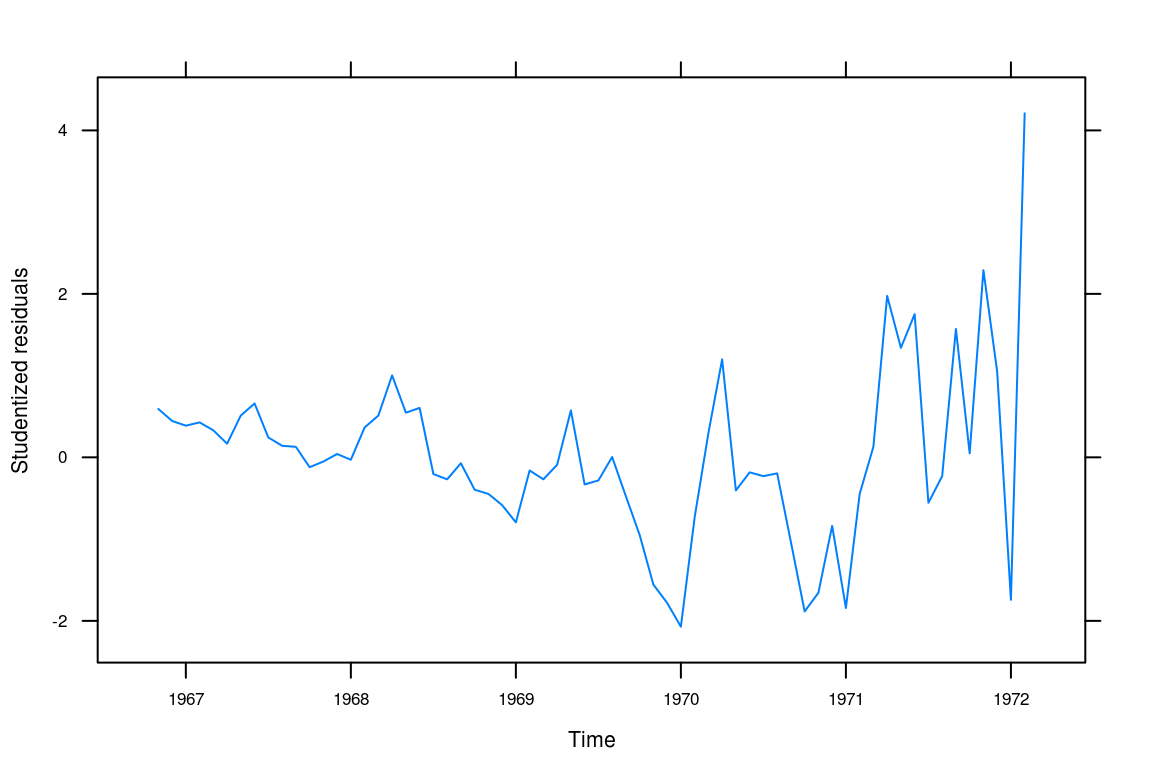
\includegraphics{TSAsolutions_files/figure-latex/winnebago-lm-res-1.pdf}
\caption{\label{fig:winnebago-lm-res}Residuals for the linear fit for the
winnebago data.}
\end{figure}

The fit is poor (Figure \ref{winnebago-lm-res}. It is not random and it
is clear that we're making worse predictions for later yers.

\subsection*{c}\label{c-13}
\addcontentsline{toc}{subsection}{c}

To produce a better fit, we transform the outcome with the natural
logarithm.

\begin{Shaded}
\begin{Highlighting}[]
\NormalTok{winn_fit_log <-}\StringTok{ }\KeywordTok{lm}\NormalTok{(}\KeywordTok{log}\NormalTok{(winnebago) ~}\StringTok{ }\KeywordTok{time}\NormalTok{(winnebago))}
\KeywordTok{pander}\NormalTok{(}\KeywordTok{summary}\NormalTok{(winn_fit_log))}
\end{Highlighting}
\end{Shaded}

\begin{longtable}[c]{@{}ccccc@{}}
\toprule
\begin{minipage}[b]{0.26\columnwidth}\centering\strut
~
\strut\end{minipage} &
\begin{minipage}[b]{0.13\columnwidth}\centering\strut
Estimate
\strut\end{minipage} &
\begin{minipage}[b]{0.16\columnwidth}\centering\strut
Std. Error
\strut\end{minipage} &
\begin{minipage}[b]{0.12\columnwidth}\centering\strut
t value
\strut\end{minipage} &
\begin{minipage}[b]{0.12\columnwidth}\centering\strut
Pr(\textgreater{}\textbar{}t\textbar{})
\strut\end{minipage}\tabularnewline
\midrule
\endhead
\begin{minipage}[t]{0.26\columnwidth}\centering\strut
\textbf{time(winnebago)}
\strut\end{minipage} &
\begin{minipage}[t]{0.13\columnwidth}\centering\strut
0.5031
\strut\end{minipage} &
\begin{minipage}[t]{0.16\columnwidth}\centering\strut
0.03199
\strut\end{minipage} &
\begin{minipage}[t]{0.12\columnwidth}\centering\strut
15.73
\strut\end{minipage} &
\begin{minipage}[t]{0.12\columnwidth}\centering\strut
2.575e-23
\strut\end{minipage}\tabularnewline
\begin{minipage}[t]{0.26\columnwidth}\centering\strut
\textbf{(Intercept)}
\strut\end{minipage} &
\begin{minipage}[t]{0.13\columnwidth}\centering\strut
-984.9
\strut\end{minipage} &
\begin{minipage}[t]{0.16\columnwidth}\centering\strut
62.99
\strut\end{minipage} &
\begin{minipage}[t]{0.12\columnwidth}\centering\strut
-15.64
\strut\end{minipage} &
\begin{minipage}[t]{0.12\columnwidth}\centering\strut
3.45e-23
\strut\end{minipage}\tabularnewline
\bottomrule
\end{longtable}

\begin{longtable}[c]{@{}cccc@{}}
\caption{Fitting linear model: log(winnebago) \textasciitilde{}
time(winnebago)}\tabularnewline
\toprule
\begin{minipage}[b]{0.18\columnwidth}\centering\strut
Observations
\strut\end{minipage} &
\begin{minipage}[b]{0.27\columnwidth}\centering\strut
Residual Std. Error
\strut\end{minipage} &
\begin{minipage}[b]{0.10\columnwidth}\centering\strut
\(R^2\)
\strut\end{minipage} &
\begin{minipage}[b]{0.20\columnwidth}\centering\strut
Adjusted \(R^2\)
\strut\end{minipage}\tabularnewline
\midrule
\endfirsthead
\toprule
\begin{minipage}[b]{0.18\columnwidth}\centering\strut
Observations
\strut\end{minipage} &
\begin{minipage}[b]{0.27\columnwidth}\centering\strut
Residual Std. Error
\strut\end{minipage} &
\begin{minipage}[b]{0.10\columnwidth}\centering\strut
\(R^2\)
\strut\end{minipage} &
\begin{minipage}[b]{0.20\columnwidth}\centering\strut
Adjusted \(R^2\)
\strut\end{minipage}\tabularnewline
\midrule
\endhead
\begin{minipage}[t]{0.18\columnwidth}\centering\strut
64
\strut\end{minipage} &
\begin{minipage}[t]{0.27\columnwidth}\centering\strut
0.3939
\strut\end{minipage} &
\begin{minipage}[t]{0.10\columnwidth}\centering\strut
0.7996
\strut\end{minipage} &
\begin{minipage}[t]{0.20\columnwidth}\centering\strut
0.7964
\strut\end{minipage}\tabularnewline
\bottomrule
\end{longtable}

The model is better, explaining almost 0.8 of the variance.

\subsection*{d}\label{d-4}
\addcontentsline{toc}{subsection}{d}

\begin{Shaded}
\begin{Highlighting}[]
\KeywordTok{xyplot}\NormalTok{(}\KeywordTok{rstudent}\NormalTok{(winn_fit_log) ~}\StringTok{ }\KeywordTok{time}\NormalTok{(winnebago), }\DataTypeTok{type =} \StringTok{"l"}\NormalTok{,}
       \DataTypeTok{xlab =} \StringTok{"Time"}\NormalTok{, }\DataTypeTok{ylab =} \StringTok{"Studentized residuals"}\NormalTok{,}
       \DataTypeTok{panel =} \NormalTok{function(x, y, ...) \{}
         \KeywordTok{panel.xyplot}\NormalTok{(x, y, ...)}
         \KeywordTok{panel.xyplot}\NormalTok{(x, y, }\DataTypeTok{pch =} \KeywordTok{as.vector}\NormalTok{(}\KeywordTok{season}\NormalTok{(winnebago)), }\DataTypeTok{col =} \DecValTok{1}\NormalTok{)}
       \NormalTok{\})}
\end{Highlighting}
\end{Shaded}

\begin{figure}[htbp]
\centering
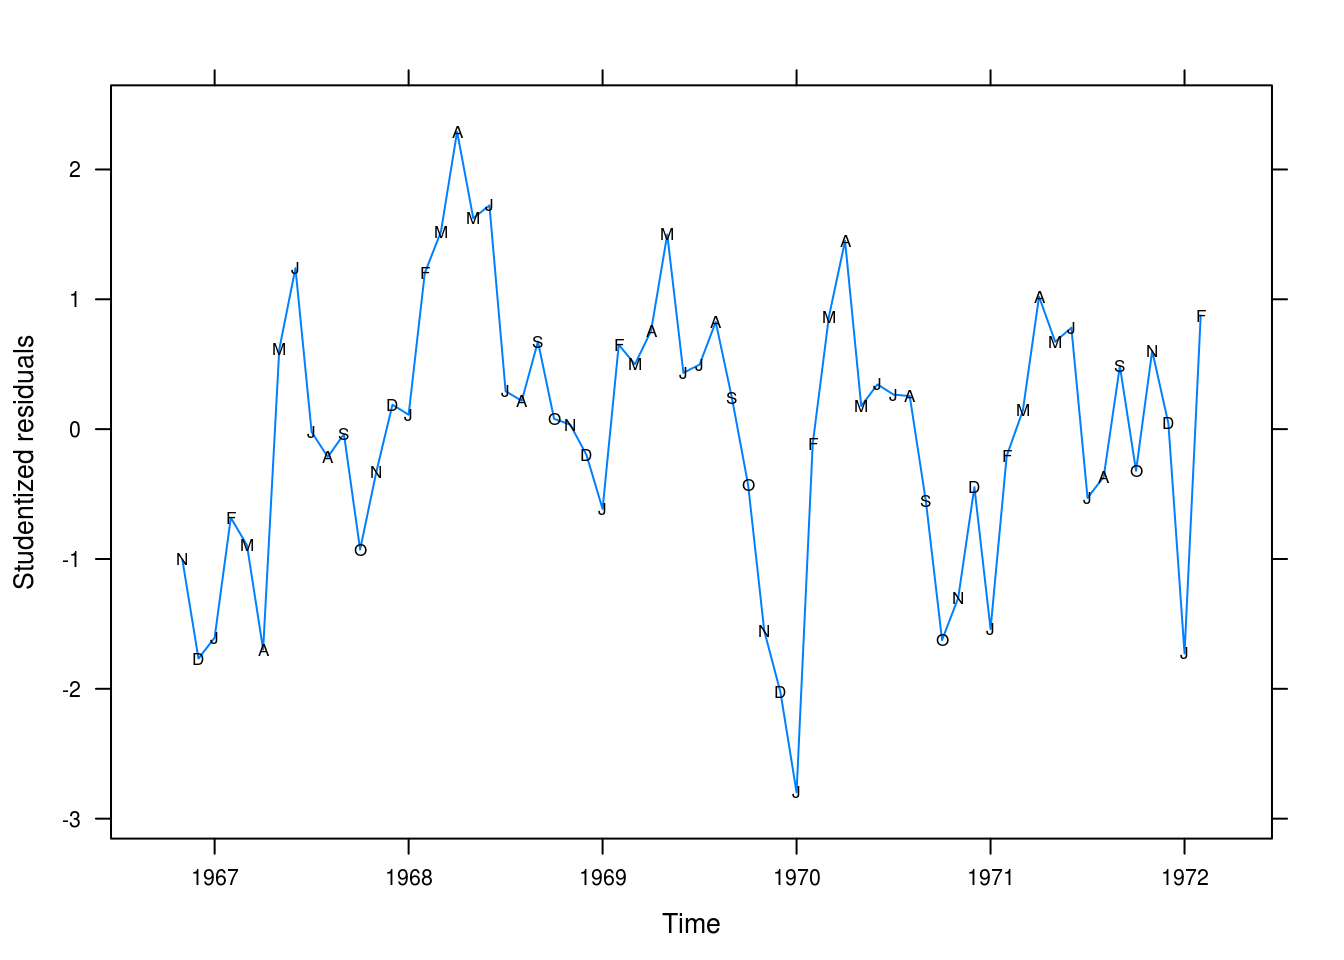
\includegraphics{TSAsolutions_files/figure-latex/winnebago-log-res-1.pdf}
\caption{\label{fig:winnebago-log-res}Residual plot after natural log
transformation.}
\end{figure}

This looks more like random noise (Figure \ref{winnebago-log-res}.
Values still cling together somewhat but it is certainly better than the
linear model. We're still systematically overpredictinig the values for
some months, however.

\subsection*{e}\label{e-3}
\addcontentsline{toc}{subsection}{e}

\begin{Shaded}
\begin{Highlighting}[]
\NormalTok{winn_fit_seasonal <-}\StringTok{ }\KeywordTok{lm}\NormalTok{(}\KeywordTok{log}\NormalTok{(winnebago) ~}\StringTok{ }\KeywordTok{season}\NormalTok{(winnebago) +}\StringTok{ }\KeywordTok{time}\NormalTok{(winnebago))}
\KeywordTok{pander}\NormalTok{(}\KeywordTok{summary}\NormalTok{(winn_fit_seasonal))}
\end{Highlighting}
\end{Shaded}

\begin{longtable}[c]{@{}ccccc@{}}
\toprule
\begin{minipage}[b]{0.37\columnwidth}\centering\strut
~
\strut\end{minipage} &
\begin{minipage}[b]{0.12\columnwidth}\centering\strut
Estimate
\strut\end{minipage} &
\begin{minipage}[b]{0.14\columnwidth}\centering\strut
Std. Error
\strut\end{minipage} &
\begin{minipage}[b]{0.11\columnwidth}\centering\strut
t value
\strut\end{minipage} &
\begin{minipage}[b]{0.11\columnwidth}\centering\strut
Pr(\textgreater{}\textbar{}t\textbar{})
\strut\end{minipage}\tabularnewline
\midrule
\endhead
\begin{minipage}[t]{0.37\columnwidth}\centering\strut
\textbf{season(winnebago)February}
\strut\end{minipage} &
\begin{minipage}[t]{0.12\columnwidth}\centering\strut
0.6244
\strut\end{minipage} &
\begin{minipage}[t]{0.14\columnwidth}\centering\strut
0.1818
\strut\end{minipage} &
\begin{minipage}[t]{0.11\columnwidth}\centering\strut
3.434
\strut\end{minipage} &
\begin{minipage}[t]{0.11\columnwidth}\centering\strut
0.001188
\strut\end{minipage}\tabularnewline
\begin{minipage}[t]{0.37\columnwidth}\centering\strut
\textbf{season(winnebago)March}
\strut\end{minipage} &
\begin{minipage}[t]{0.12\columnwidth}\centering\strut
0.6822
\strut\end{minipage} &
\begin{minipage}[t]{0.14\columnwidth}\centering\strut
0.1909
\strut\end{minipage} &
\begin{minipage}[t]{0.11\columnwidth}\centering\strut
3.574
\strut\end{minipage} &
\begin{minipage}[t]{0.11\columnwidth}\centering\strut
0.0007793
\strut\end{minipage}\tabularnewline
\begin{minipage}[t]{0.37\columnwidth}\centering\strut
\textbf{season(winnebago)April}
\strut\end{minipage} &
\begin{minipage}[t]{0.12\columnwidth}\centering\strut
0.8096
\strut\end{minipage} &
\begin{minipage}[t]{0.14\columnwidth}\centering\strut
0.1908
\strut\end{minipage} &
\begin{minipage}[t]{0.11\columnwidth}\centering\strut
4.243
\strut\end{minipage} &
\begin{minipage}[t]{0.11\columnwidth}\centering\strut
9.301e-05
\strut\end{minipage}\tabularnewline
\begin{minipage}[t]{0.37\columnwidth}\centering\strut
\textbf{season(winnebago)May}
\strut\end{minipage} &
\begin{minipage}[t]{0.12\columnwidth}\centering\strut
0.8695
\strut\end{minipage} &
\begin{minipage}[t]{0.14\columnwidth}\centering\strut
0.1907
\strut\end{minipage} &
\begin{minipage}[t]{0.11\columnwidth}\centering\strut
4.559
\strut\end{minipage} &
\begin{minipage}[t]{0.11\columnwidth}\centering\strut
3.246e-05
\strut\end{minipage}\tabularnewline
\begin{minipage}[t]{0.37\columnwidth}\centering\strut
\textbf{season(winnebago)June}
\strut\end{minipage} &
\begin{minipage}[t]{0.12\columnwidth}\centering\strut
0.8631
\strut\end{minipage} &
\begin{minipage}[t]{0.14\columnwidth}\centering\strut
0.1907
\strut\end{minipage} &
\begin{minipage}[t]{0.11\columnwidth}\centering\strut
4.526
\strut\end{minipage} &
\begin{minipage}[t]{0.11\columnwidth}\centering\strut
3.627e-05
\strut\end{minipage}\tabularnewline
\begin{minipage}[t]{0.37\columnwidth}\centering\strut
\textbf{season(winnebago)July}
\strut\end{minipage} &
\begin{minipage}[t]{0.12\columnwidth}\centering\strut
0.5539
\strut\end{minipage} &
\begin{minipage}[t]{0.14\columnwidth}\centering\strut
0.1907
\strut\end{minipage} &
\begin{minipage}[t]{0.11\columnwidth}\centering\strut
2.905
\strut\end{minipage} &
\begin{minipage}[t]{0.11\columnwidth}\centering\strut
0.00542
\strut\end{minipage}\tabularnewline
\begin{minipage}[t]{0.37\columnwidth}\centering\strut
\textbf{season(winnebago)August}
\strut\end{minipage} &
\begin{minipage}[t]{0.12\columnwidth}\centering\strut
0.5699
\strut\end{minipage} &
\begin{minipage}[t]{0.14\columnwidth}\centering\strut
0.1907
\strut\end{minipage} &
\begin{minipage}[t]{0.11\columnwidth}\centering\strut
2.988
\strut\end{minipage} &
\begin{minipage}[t]{0.11\columnwidth}\centering\strut
0.004305
\strut\end{minipage}\tabularnewline
\begin{minipage}[t]{0.37\columnwidth}\centering\strut
\textbf{season(winnebago)September}
\strut\end{minipage} &
\begin{minipage}[t]{0.12\columnwidth}\centering\strut
0.5757
\strut\end{minipage} &
\begin{minipage}[t]{0.14\columnwidth}\centering\strut
0.1907
\strut\end{minipage} &
\begin{minipage}[t]{0.11\columnwidth}\centering\strut
3.018
\strut\end{minipage} &
\begin{minipage}[t]{0.11\columnwidth}\centering\strut
0.00396
\strut\end{minipage}\tabularnewline
\begin{minipage}[t]{0.37\columnwidth}\centering\strut
\textbf{season(winnebago)October}
\strut\end{minipage} &
\begin{minipage}[t]{0.12\columnwidth}\centering\strut
0.2635
\strut\end{minipage} &
\begin{minipage}[t]{0.14\columnwidth}\centering\strut
0.1908
\strut\end{minipage} &
\begin{minipage}[t]{0.11\columnwidth}\centering\strut
1.381
\strut\end{minipage} &
\begin{minipage}[t]{0.11\columnwidth}\centering\strut
0.1733
\strut\end{minipage}\tabularnewline
\begin{minipage}[t]{0.37\columnwidth}\centering\strut
\textbf{season(winnebago)November}
\strut\end{minipage} &
\begin{minipage}[t]{0.12\columnwidth}\centering\strut
0.2868
\strut\end{minipage} &
\begin{minipage}[t]{0.14\columnwidth}\centering\strut
0.1819
\strut\end{minipage} &
\begin{minipage}[t]{0.11\columnwidth}\centering\strut
1.577
\strut\end{minipage} &
\begin{minipage}[t]{0.11\columnwidth}\centering\strut
0.1209
\strut\end{minipage}\tabularnewline
\begin{minipage}[t]{0.37\columnwidth}\centering\strut
\textbf{season(winnebago)December}
\strut\end{minipage} &
\begin{minipage}[t]{0.12\columnwidth}\centering\strut
0.248
\strut\end{minipage} &
\begin{minipage}[t]{0.14\columnwidth}\centering\strut
0.1818
\strut\end{minipage} &
\begin{minipage}[t]{0.11\columnwidth}\centering\strut
1.364
\strut\end{minipage} &
\begin{minipage}[t]{0.11\columnwidth}\centering\strut
0.1785
\strut\end{minipage}\tabularnewline
\begin{minipage}[t]{0.37\columnwidth}\centering\strut
\textbf{time(winnebago)}
\strut\end{minipage} &
\begin{minipage}[t]{0.12\columnwidth}\centering\strut
0.5091
\strut\end{minipage} &
\begin{minipage}[t]{0.14\columnwidth}\centering\strut
0.02571
\strut\end{minipage} &
\begin{minipage}[t]{0.11\columnwidth}\centering\strut
19.8
\strut\end{minipage} &
\begin{minipage}[t]{0.11\columnwidth}\centering\strut
1.351e-25
\strut\end{minipage}\tabularnewline
\begin{minipage}[t]{0.37\columnwidth}\centering\strut
\textbf{(Intercept)}
\strut\end{minipage} &
\begin{minipage}[t]{0.12\columnwidth}\centering\strut
-997.3
\strut\end{minipage} &
\begin{minipage}[t]{0.14\columnwidth}\centering\strut
50.64
\strut\end{minipage} &
\begin{minipage}[t]{0.11\columnwidth}\centering\strut
-19.69
\strut\end{minipage} &
\begin{minipage}[t]{0.11\columnwidth}\centering\strut
1.718e-25
\strut\end{minipage}\tabularnewline
\bottomrule
\end{longtable}

\begin{longtable}[c]{@{}cccc@{}}
\caption{Fitting linear model: log(winnebago) \textasciitilde{}
season(winnebago) + time(winnebago)}\tabularnewline
\toprule
\begin{minipage}[b]{0.18\columnwidth}\centering\strut
Observations
\strut\end{minipage} &
\begin{minipage}[b]{0.27\columnwidth}\centering\strut
Residual Std. Error
\strut\end{minipage} &
\begin{minipage}[b]{0.10\columnwidth}\centering\strut
\(R^2\)
\strut\end{minipage} &
\begin{minipage}[b]{0.20\columnwidth}\centering\strut
Adjusted \(R^2\)
\strut\end{minipage}\tabularnewline
\midrule
\endfirsthead
\toprule
\begin{minipage}[b]{0.18\columnwidth}\centering\strut
Observations
\strut\end{minipage} &
\begin{minipage}[b]{0.27\columnwidth}\centering\strut
Residual Std. Error
\strut\end{minipage} &
\begin{minipage}[b]{0.10\columnwidth}\centering\strut
\(R^2\)
\strut\end{minipage} &
\begin{minipage}[b]{0.20\columnwidth}\centering\strut
Adjusted \(R^2\)
\strut\end{minipage}\tabularnewline
\midrule
\endhead
\begin{minipage}[t]{0.18\columnwidth}\centering\strut
64
\strut\end{minipage} &
\begin{minipage}[t]{0.27\columnwidth}\centering\strut
0.3149
\strut\end{minipage} &
\begin{minipage}[t]{0.10\columnwidth}\centering\strut
0.8946
\strut\end{minipage} &
\begin{minipage}[t]{0.20\columnwidth}\centering\strut
0.8699
\strut\end{minipage}\tabularnewline
\bottomrule
\end{longtable}

The fit is improved further. We have a R\textsuperscript{2} of 0.89 and
significance for most of our seasonal means as well as the time trend.

\subsection*{f}\label{f-1}
\addcontentsline{toc}{subsection}{f}

\begin{Shaded}
\begin{Highlighting}[]
\KeywordTok{xyplot}\NormalTok{(}\KeywordTok{rstudent}\NormalTok{(winn_fit_seasonal) ~}\StringTok{ }\KeywordTok{time}\NormalTok{(winnebago), }\DataTypeTok{type =} \StringTok{"l"}\NormalTok{,}
       \DataTypeTok{xlab =} \StringTok{"Time"}\NormalTok{, }\DataTypeTok{ylab =} \StringTok{"Studentized residuals"}\NormalTok{,}
       \DataTypeTok{panel =} \NormalTok{function(x, y, ...) \{}
         \KeywordTok{panel.xyplot}\NormalTok{(x, y, ...)}
         \KeywordTok{panel.xyplot}\NormalTok{(x, y, }\DataTypeTok{col =} \DecValTok{1}\NormalTok{, }\DataTypeTok{pch =} \KeywordTok{as.vector}\NormalTok{(}\KeywordTok{season}\NormalTok{(winnebago)))}
       \NormalTok{\})}
\end{Highlighting}
\end{Shaded}

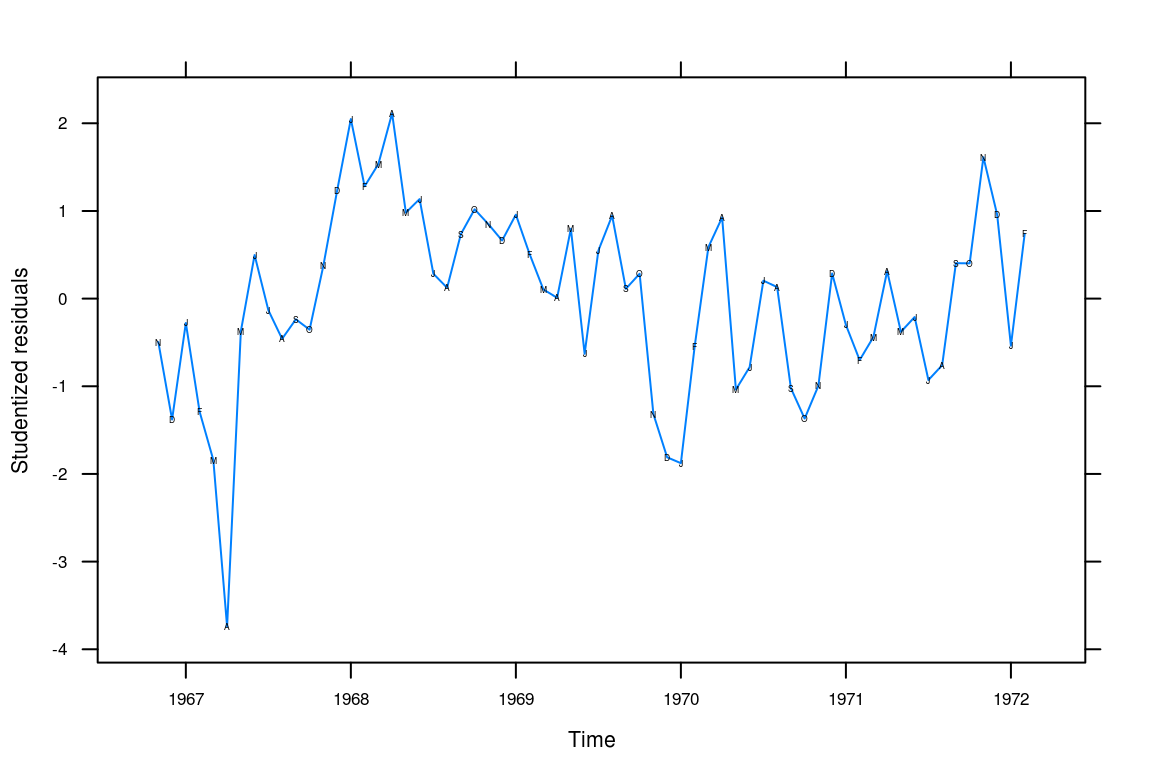
\includegraphics{TSAsolutions_files/figure-latex/unnamed-chunk-23-1.pdf}

This is acceptable even if our residuals are quite large for some of the
values, notably at the start of the series.

\section{Retail}\label{retail}

\subsection*{a}\label{a-25}
\addcontentsline{toc}{subsection}{a}

\begin{Shaded}
\begin{Highlighting}[]
\KeywordTok{data}\NormalTok{(retail)}
\KeywordTok{xyplot}\NormalTok{(retail, }\DataTypeTok{panel =} \NormalTok{function(x, y, ...) \{}
  \KeywordTok{panel.xyplot}\NormalTok{(x, y, ...)}
  \KeywordTok{panel.xyplot}\NormalTok{(x, y, }\DataTypeTok{pch =} \KeywordTok{as.vector}\NormalTok{(}\KeywordTok{season}\NormalTok{(retail)), }\DataTypeTok{col =} \DecValTok{1}\NormalTok{)}
\NormalTok{\})}
\end{Highlighting}
\end{Shaded}

\begin{figure}[htbp]
\centering
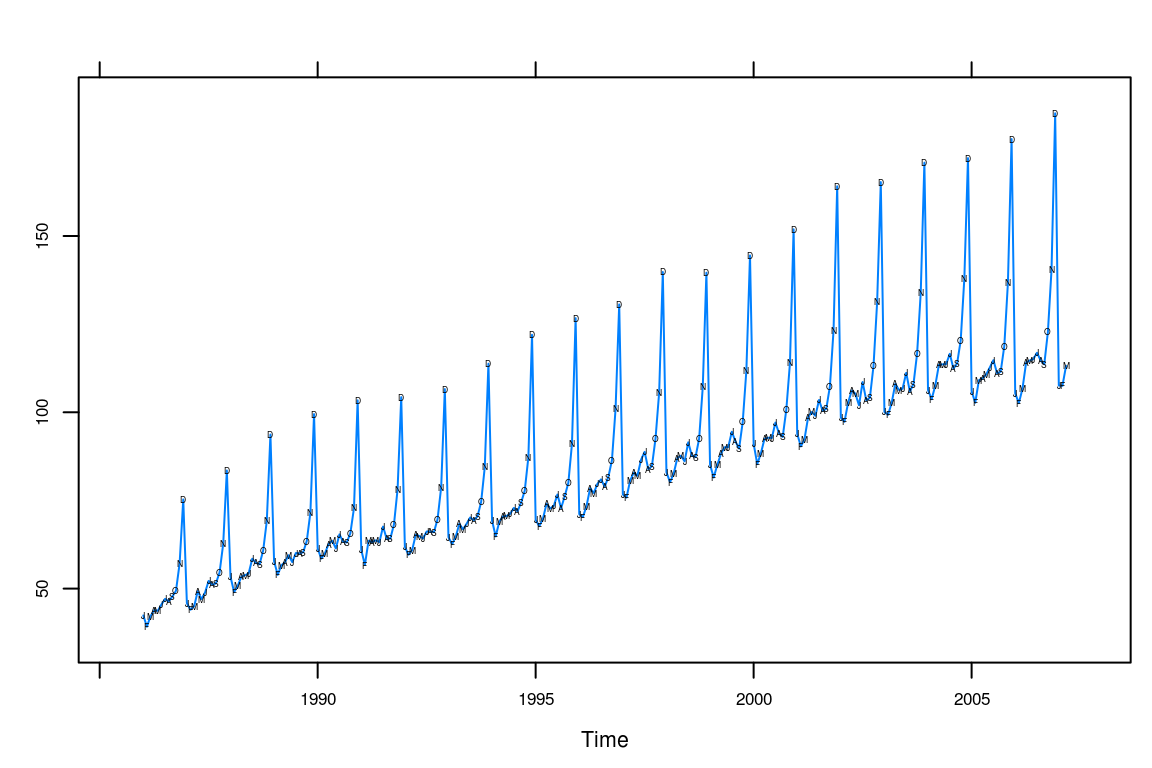
\includegraphics{TSAsolutions_files/figure-latex/unnamed-chunk-24-1.pdf}
\caption{\label{fig:unnamed-chunk-24}Total retail sales in the U.K. in
billions pounds.}
\end{figure}

Plotting the retail sales trend there seems to be a long-term linear
trend as well as heavy seasonality in tht December -- and to slighter
extent also November and October -- exhibit regular surges in retail
sales.

\subsection*{b}\label{b-25}
\addcontentsline{toc}{subsection}{b}

\begin{Shaded}
\begin{Highlighting}[]
\NormalTok{retail_lm <-}\StringTok{ }\KeywordTok{lm}\NormalTok{(retail ~}\StringTok{ }\KeywordTok{season}\NormalTok{(retail) +}\StringTok{ }\KeywordTok{time}\NormalTok{(retail))}
\KeywordTok{pander}\NormalTok{(}\KeywordTok{summary}\NormalTok{(retail_lm))}
\end{Highlighting}
\end{Shaded}

\begin{longtable}[c]{@{}ccccc@{}}
\toprule
\begin{minipage}[b]{0.35\columnwidth}\centering\strut
~
\strut\end{minipage} &
\begin{minipage}[b]{0.13\columnwidth}\centering\strut
Estimate
\strut\end{minipage} &
\begin{minipage}[b]{0.15\columnwidth}\centering\strut
Std. Error
\strut\end{minipage} &
\begin{minipage}[b]{0.12\columnwidth}\centering\strut
t value
\strut\end{minipage} &
\begin{minipage}[b]{0.12\columnwidth}\centering\strut
Pr(\textgreater{}\textbar{}t\textbar{})
\strut\end{minipage}\tabularnewline
\midrule
\endhead
\begin{minipage}[t]{0.35\columnwidth}\centering\strut
\textbf{season(retail)February}
\strut\end{minipage} &
\begin{minipage}[t]{0.13\columnwidth}\centering\strut
-3.015
\strut\end{minipage} &
\begin{minipage}[t]{0.15\columnwidth}\centering\strut
1.29
\strut\end{minipage} &
\begin{minipage}[t]{0.12\columnwidth}\centering\strut
-2.337
\strut\end{minipage} &
\begin{minipage}[t]{0.12\columnwidth}\centering\strut
0.02024
\strut\end{minipage}\tabularnewline
\begin{minipage}[t]{0.35\columnwidth}\centering\strut
\textbf{season(retail)March}
\strut\end{minipage} &
\begin{minipage}[t]{0.13\columnwidth}\centering\strut
0.07469
\strut\end{minipage} &
\begin{minipage}[t]{0.15\columnwidth}\centering\strut
1.29
\strut\end{minipage} &
\begin{minipage}[t]{0.12\columnwidth}\centering\strut
0.05791
\strut\end{minipage} &
\begin{minipage}[t]{0.12\columnwidth}\centering\strut
0.9539
\strut\end{minipage}\tabularnewline
\begin{minipage}[t]{0.35\columnwidth}\centering\strut
\textbf{season(retail)April}
\strut\end{minipage} &
\begin{minipage}[t]{0.13\columnwidth}\centering\strut
3.447
\strut\end{minipage} &
\begin{minipage}[t]{0.15\columnwidth}\centering\strut
1.305
\strut\end{minipage} &
\begin{minipage}[t]{0.12\columnwidth}\centering\strut
2.641
\strut\end{minipage} &
\begin{minipage}[t]{0.12\columnwidth}\centering\strut
0.008801
\strut\end{minipage}\tabularnewline
\begin{minipage}[t]{0.35\columnwidth}\centering\strut
\textbf{season(retail)May}
\strut\end{minipage} &
\begin{minipage}[t]{0.13\columnwidth}\centering\strut
3.108
\strut\end{minipage} &
\begin{minipage}[t]{0.15\columnwidth}\centering\strut
1.305
\strut\end{minipage} &
\begin{minipage}[t]{0.12\columnwidth}\centering\strut
2.381
\strut\end{minipage} &
\begin{minipage}[t]{0.12\columnwidth}\centering\strut
0.01803
\strut\end{minipage}\tabularnewline
\begin{minipage}[t]{0.35\columnwidth}\centering\strut
\textbf{season(retail)June}
\strut\end{minipage} &
\begin{minipage}[t]{0.13\columnwidth}\centering\strut
3.074
\strut\end{minipage} &
\begin{minipage}[t]{0.15\columnwidth}\centering\strut
1.305
\strut\end{minipage} &
\begin{minipage}[t]{0.12\columnwidth}\centering\strut
2.355
\strut\end{minipage} &
\begin{minipage}[t]{0.12\columnwidth}\centering\strut
0.01932
\strut\end{minipage}\tabularnewline
\begin{minipage}[t]{0.35\columnwidth}\centering\strut
\textbf{season(retail)July}
\strut\end{minipage} &
\begin{minipage}[t]{0.13\columnwidth}\centering\strut
6.053
\strut\end{minipage} &
\begin{minipage}[t]{0.15\columnwidth}\centering\strut
1.305
\strut\end{minipage} &
\begin{minipage}[t]{0.12\columnwidth}\centering\strut
4.638
\strut\end{minipage} &
\begin{minipage}[t]{0.12\columnwidth}\centering\strut
5.757e-06
\strut\end{minipage}\tabularnewline
\begin{minipage}[t]{0.35\columnwidth}\centering\strut
\textbf{season(retail)August}
\strut\end{minipage} &
\begin{minipage}[t]{0.13\columnwidth}\centering\strut
3.138
\strut\end{minipage} &
\begin{minipage}[t]{0.15\columnwidth}\centering\strut
1.305
\strut\end{minipage} &
\begin{minipage}[t]{0.12\columnwidth}\centering\strut
2.404
\strut\end{minipage} &
\begin{minipage}[t]{0.12\columnwidth}\centering\strut
0.01695
\strut\end{minipage}\tabularnewline
\begin{minipage}[t]{0.35\columnwidth}\centering\strut
\textbf{season(retail)September}
\strut\end{minipage} &
\begin{minipage}[t]{0.13\columnwidth}\centering\strut
3.428
\strut\end{minipage} &
\begin{minipage}[t]{0.15\columnwidth}\centering\strut
1.305
\strut\end{minipage} &
\begin{minipage}[t]{0.12\columnwidth}\centering\strut
2.626
\strut\end{minipage} &
\begin{minipage}[t]{0.12\columnwidth}\centering\strut
0.009187
\strut\end{minipage}\tabularnewline
\begin{minipage}[t]{0.35\columnwidth}\centering\strut
\textbf{season(retail)October}
\strut\end{minipage} &
\begin{minipage}[t]{0.13\columnwidth}\centering\strut
8.555
\strut\end{minipage} &
\begin{minipage}[t]{0.15\columnwidth}\centering\strut
1.305
\strut\end{minipage} &
\begin{minipage}[t]{0.12\columnwidth}\centering\strut
6.555
\strut\end{minipage} &
\begin{minipage}[t]{0.12\columnwidth}\centering\strut
3.336e-10
\strut\end{minipage}\tabularnewline
\begin{minipage}[t]{0.35\columnwidth}\centering\strut
\textbf{season(retail)November}
\strut\end{minipage} &
\begin{minipage}[t]{0.13\columnwidth}\centering\strut
20.82
\strut\end{minipage} &
\begin{minipage}[t]{0.15\columnwidth}\centering\strut
1.305
\strut\end{minipage} &
\begin{minipage}[t]{0.12\columnwidth}\centering\strut
15.95
\strut\end{minipage} &
\begin{minipage}[t]{0.12\columnwidth}\centering\strut
1.274e-39
\strut\end{minipage}\tabularnewline
\begin{minipage}[t]{0.35\columnwidth}\centering\strut
\textbf{season(retail)December}
\strut\end{minipage} &
\begin{minipage}[t]{0.13\columnwidth}\centering\strut
52.54
\strut\end{minipage} &
\begin{minipage}[t]{0.15\columnwidth}\centering\strut
1.305
\strut\end{minipage} &
\begin{minipage}[t]{0.12\columnwidth}\centering\strut
40.25
\strut\end{minipage} &
\begin{minipage}[t]{0.12\columnwidth}\centering\strut
3.169e-109
\strut\end{minipage}\tabularnewline
\begin{minipage}[t]{0.35\columnwidth}\centering\strut
\textbf{time(retail)}
\strut\end{minipage} &
\begin{minipage}[t]{0.13\columnwidth}\centering\strut
3.67
\strut\end{minipage} &
\begin{minipage}[t]{0.15\columnwidth}\centering\strut
0.04369
\strut\end{minipage} &
\begin{minipage}[t]{0.12\columnwidth}\centering\strut
84
\strut\end{minipage} &
\begin{minipage}[t]{0.12\columnwidth}\centering\strut
5.206e-181
\strut\end{minipage}\tabularnewline
\begin{minipage}[t]{0.35\columnwidth}\centering\strut
\textbf{(Intercept)}
\strut\end{minipage} &
\begin{minipage}[t]{0.13\columnwidth}\centering\strut
-7249
\strut\end{minipage} &
\begin{minipage}[t]{0.15\columnwidth}\centering\strut
87.24
\strut\end{minipage} &
\begin{minipage}[t]{0.12\columnwidth}\centering\strut
-83.1
\strut\end{minipage} &
\begin{minipage}[t]{0.12\columnwidth}\centering\strut
6.41e-180
\strut\end{minipage}\tabularnewline
\bottomrule
\end{longtable}

\begin{longtable}[c]{@{}cccc@{}}
\caption{Fitting linear model: retail \textasciitilde{} season(retail) +
time(retail)}\tabularnewline
\toprule
\begin{minipage}[b]{0.18\columnwidth}\centering\strut
Observations
\strut\end{minipage} &
\begin{minipage}[b]{0.27\columnwidth}\centering\strut
Residual Std. Error
\strut\end{minipage} &
\begin{minipage}[b]{0.10\columnwidth}\centering\strut
\(R^2\)
\strut\end{minipage} &
\begin{minipage}[b]{0.20\columnwidth}\centering\strut
Adjusted \(R^2\)
\strut\end{minipage}\tabularnewline
\midrule
\endfirsthead
\toprule
\begin{minipage}[b]{0.18\columnwidth}\centering\strut
Observations
\strut\end{minipage} &
\begin{minipage}[b]{0.27\columnwidth}\centering\strut
Residual Std. Error
\strut\end{minipage} &
\begin{minipage}[b]{0.10\columnwidth}\centering\strut
\(R^2\)
\strut\end{minipage} &
\begin{minipage}[b]{0.20\columnwidth}\centering\strut
Adjusted \(R^2\)
\strut\end{minipage}\tabularnewline
\midrule
\endhead
\begin{minipage}[t]{0.18\columnwidth}\centering\strut
255
\strut\end{minipage} &
\begin{minipage}[t]{0.27\columnwidth}\centering\strut
4.278
\strut\end{minipage} &
\begin{minipage}[t]{0.10\columnwidth}\centering\strut
0.9767
\strut\end{minipage} &
\begin{minipage}[t]{0.20\columnwidth}\centering\strut
0.9755
\strut\end{minipage}\tabularnewline
\bottomrule
\end{longtable}

This \emph{seems} like an effective model, explaining 0.98 of the
variance in retail sales.

\subsection*{c}\label{c-14}
\addcontentsline{toc}{subsection}{c}

\begin{Shaded}
\begin{Highlighting}[]
\KeywordTok{xyplot}\NormalTok{(}\KeywordTok{rstudent}\NormalTok{(retail_lm) ~}\StringTok{ }\KeywordTok{time}\NormalTok{(retail), }\DataTypeTok{type =} \StringTok{"l"}\NormalTok{,}
       \DataTypeTok{xlab =} \StringTok{"Time"}\NormalTok{, }\DataTypeTok{ylab =} \StringTok{"Studentized residuals"}\NormalTok{,}
       \DataTypeTok{panel =} \NormalTok{function(x, y, ...) \{}
         \KeywordTok{panel.xyplot}\NormalTok{(x, y, ...)}
         \KeywordTok{panel.xyplot}\NormalTok{(x, y, }\DataTypeTok{pch =} \KeywordTok{as.vector}\NormalTok{(}\KeywordTok{season}\NormalTok{(retail)), }\DataTypeTok{col =} \DecValTok{1}\NormalTok{)}
       \NormalTok{\})}
\end{Highlighting}
\end{Shaded}

\begin{figure}[htbp]
\centering
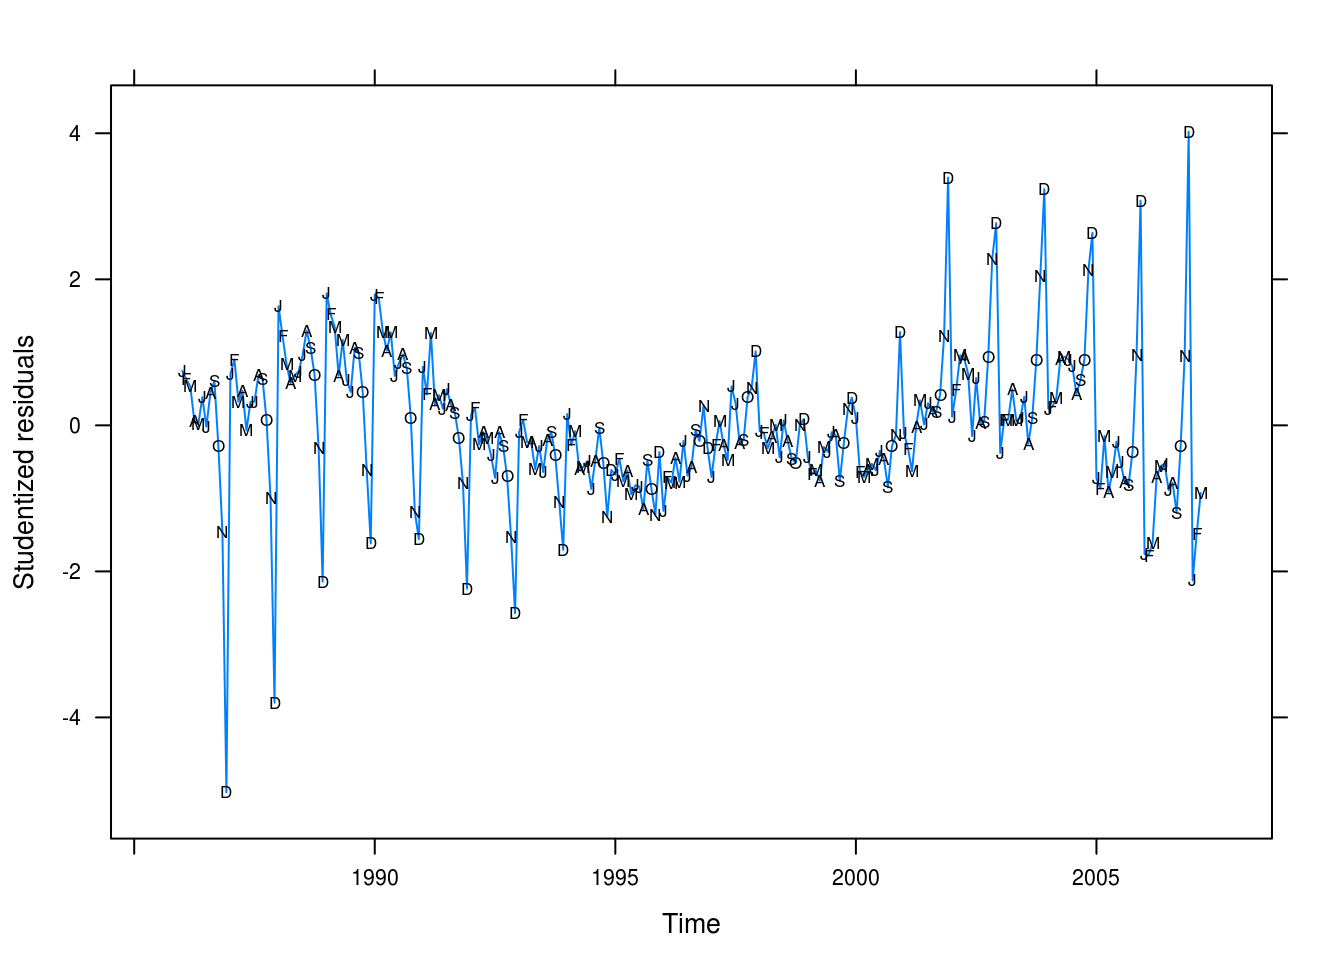
\includegraphics{TSAsolutions_files/figure-latex/retail-res-1.pdf}
\caption{\label{fig:retail-res}Studentized residuals for our seasonality +
linear model of retail sales.}
\end{figure}

The residual plot (Figure \ref{fig:retail-res}) tells a different story:
we're underpredicting values for early period and overpredicting values
for the later years -- however, this should be an easy fix.

\section{Prescriptions}\label{prescriptions}

\subsection*{a}\label{a-26}
\addcontentsline{toc}{subsection}{a}

\begin{Shaded}
\begin{Highlighting}[]
\KeywordTok{data}\NormalTok{(prescrip)}
\KeywordTok{xyplot}\NormalTok{(prescrip, }\DataTypeTok{ylab =} \StringTok{"Prescription costs"}\NormalTok{,}
       \DataTypeTok{panel =} \NormalTok{function(x, y, ...) \{}
         \KeywordTok{panel.xyplot}\NormalTok{(x, y, ...)}
         \KeywordTok{panel.xyplot}\NormalTok{(x, y, }\DataTypeTok{pch =} \KeywordTok{as.vector}\NormalTok{(}\KeywordTok{season}\NormalTok{(prescrip)), }\DataTypeTok{col =} \DecValTok{1}\NormalTok{)}
       \NormalTok{\})}
\end{Highlighting}
\end{Shaded}

\begin{figure}[htbp]
\centering
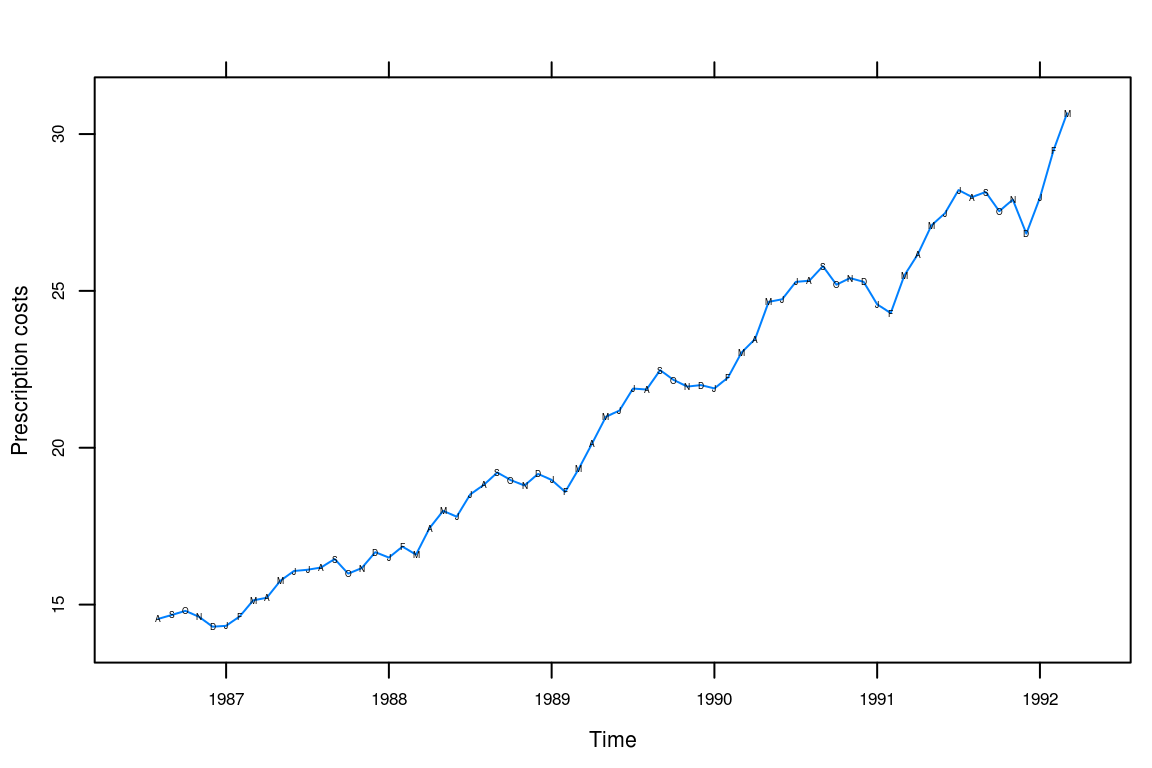
\includegraphics{TSAsolutions_files/figure-latex/prescrip-1.pdf}
\caption{\label{fig:prescrip}Monthly U.S. prescription costs.}
\end{figure}

Figure \ref{fig:prescrip} shows a clear, smooth, and cyclical seasonal
trend. Values are genereally higher for the summer months and there
seems to be an exponential increase long-term.

\subsection*{b}\label{b-26}
\addcontentsline{toc}{subsection}{b}

\begin{Shaded}
\begin{Highlighting}[]
\NormalTok{pchange <-}\StringTok{ }\KeywordTok{diff}\NormalTok{(prescrip) /}\StringTok{ }\NormalTok{prescrip}
\KeywordTok{xyplot}\NormalTok{(pchange ~}\StringTok{ }\KeywordTok{time}\NormalTok{(prescrip), }\DataTypeTok{type =} \StringTok{"l"}\NormalTok{,}
       \DataTypeTok{panel =} \NormalTok{function(x, y, ...) \{}
         \KeywordTok{panel.xyplot}\NormalTok{(x, y, ...)}
         \KeywordTok{panel.xyplot}\NormalTok{(x, y, }\DataTypeTok{pch =} \KeywordTok{as.vector}\NormalTok{(}\KeywordTok{season}\NormalTok{(pchange)), }\DataTypeTok{col =} \DecValTok{1}\NormalTok{)}
       \NormalTok{\})}
\end{Highlighting}
\end{Shaded}

\begin{figure}[htbp]
\centering
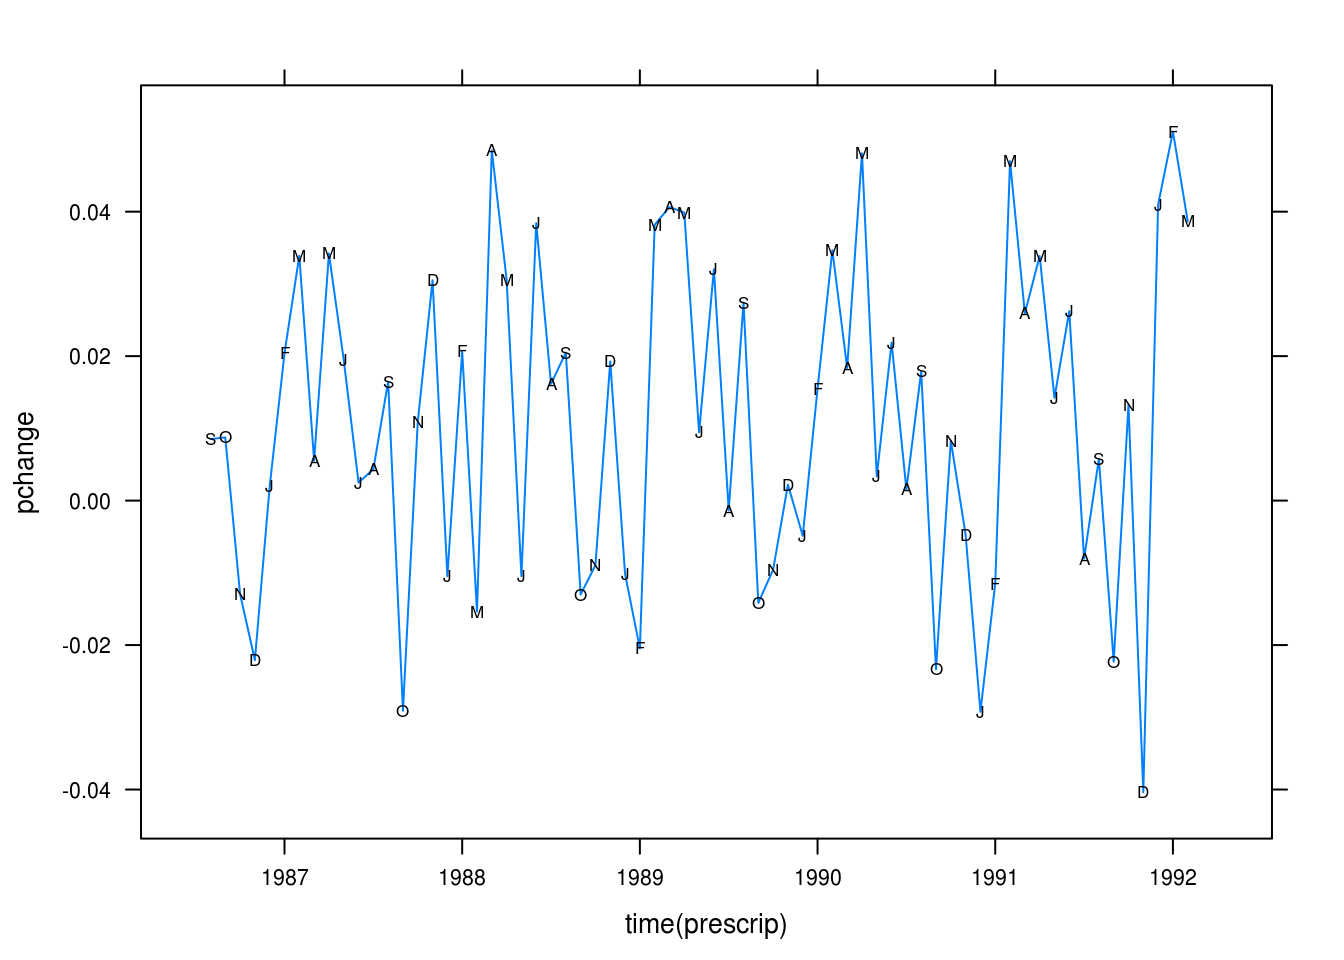
\includegraphics{TSAsolutions_files/figure-latex/prescrip-diff-1.pdf}
\caption{\label{fig:prescrip-diff}Percentage changes from month-to-month in
prescription costs.}
\end{figure}

The monthly percentage difference series looks rather stationary.

\subsection*{c}\label{c-15}
\addcontentsline{toc}{subsection}{c}

\begin{Shaded}
\begin{Highlighting}[]
\NormalTok{pres_cos <-}\StringTok{ }\KeywordTok{lm}\NormalTok{(pchange ~}\StringTok{ }\KeywordTok{harmonic}\NormalTok{(pchange))}
\KeywordTok{pander}\NormalTok{(}\KeywordTok{summary}\NormalTok{(pres_cos))}
\end{Highlighting}
\end{Shaded}

\begin{longtable}[c]{@{}ccccc@{}}
\toprule
\begin{minipage}[b]{0.38\columnwidth}\centering\strut
~
\strut\end{minipage} &
\begin{minipage}[b]{0.12\columnwidth}\centering\strut
Estimate
\strut\end{minipage} &
\begin{minipage}[b]{0.14\columnwidth}\centering\strut
Std. Error
\strut\end{minipage} &
\begin{minipage}[b]{0.11\columnwidth}\centering\strut
t value
\strut\end{minipage} &
\begin{minipage}[b]{0.11\columnwidth}\centering\strut
Pr(\textgreater{}\textbar{}t\textbar{})
\strut\end{minipage}\tabularnewline
\midrule
\endhead
\begin{minipage}[t]{0.38\columnwidth}\centering\strut
\textbf{harmonic(pchange)cos(2\emph{pi}t)}
\strut\end{minipage} &
\begin{minipage}[t]{0.12\columnwidth}\centering\strut
-0.006605
\strut\end{minipage} &
\begin{minipage}[t]{0.14\columnwidth}\centering\strut
0.003237
\strut\end{minipage} &
\begin{minipage}[t]{0.11\columnwidth}\centering\strut
-2.041
\strut\end{minipage} &
\begin{minipage}[t]{0.11\columnwidth}\centering\strut
0.04542
\strut\end{minipage}\tabularnewline
\begin{minipage}[t]{0.38\columnwidth}\centering\strut
\textbf{harmonic(pchange)sin(2\emph{pi}t)}
\strut\end{minipage} &
\begin{minipage}[t]{0.12\columnwidth}\centering\strut
0.01612
\strut\end{minipage} &
\begin{minipage}[t]{0.14\columnwidth}\centering\strut
0.003208
\strut\end{minipage} &
\begin{minipage}[t]{0.11\columnwidth}\centering\strut
5.026
\strut\end{minipage} &
\begin{minipage}[t]{0.11\columnwidth}\centering\strut
4.291e-06
\strut\end{minipage}\tabularnewline
\begin{minipage}[t]{0.38\columnwidth}\centering\strut
\textbf{(Intercept)}
\strut\end{minipage} &
\begin{minipage}[t]{0.12\columnwidth}\centering\strut
0.01159
\strut\end{minipage} &
\begin{minipage}[t]{0.14\columnwidth}\centering\strut
0.002282
\strut\end{minipage} &
\begin{minipage}[t]{0.11\columnwidth}\centering\strut
5.08
\strut\end{minipage} &
\begin{minipage}[t]{0.11\columnwidth}\centering\strut
3.508e-06
\strut\end{minipage}\tabularnewline
\bottomrule
\end{longtable}

\begin{longtable}[c]{@{}cccc@{}}
\caption{Fitting linear model: pchange \textasciitilde{}
harmonic(pchange)}\tabularnewline
\toprule
\begin{minipage}[b]{0.18\columnwidth}\centering\strut
Observations
\strut\end{minipage} &
\begin{minipage}[b]{0.27\columnwidth}\centering\strut
Residual Std. Error
\strut\end{minipage} &
\begin{minipage}[b]{0.10\columnwidth}\centering\strut
\(R^2\)
\strut\end{minipage} &
\begin{minipage}[b]{0.20\columnwidth}\centering\strut
Adjusted \(R^2\)
\strut\end{minipage}\tabularnewline
\midrule
\endfirsthead
\toprule
\begin{minipage}[b]{0.18\columnwidth}\centering\strut
Observations
\strut\end{minipage} &
\begin{minipage}[b]{0.27\columnwidth}\centering\strut
Residual Std. Error
\strut\end{minipage} &
\begin{minipage}[b]{0.10\columnwidth}\centering\strut
\(R^2\)
\strut\end{minipage} &
\begin{minipage}[b]{0.20\columnwidth}\centering\strut
Adjusted \(R^2\)
\strut\end{minipage}\tabularnewline
\midrule
\endhead
\begin{minipage}[t]{0.18\columnwidth}\centering\strut
67
\strut\end{minipage} &
\begin{minipage}[t]{0.27\columnwidth}\centering\strut
0.01862
\strut\end{minipage} &
\begin{minipage}[t]{0.10\columnwidth}\centering\strut
0.3126
\strut\end{minipage} &
\begin{minipage}[t]{0.20\columnwidth}\centering\strut
0.2912
\strut\end{minipage}\tabularnewline
\bottomrule
\end{longtable}

We explain 0.31 of the variance. The model is significant though.

\subsection*{d}\label{d-5}
\addcontentsline{toc}{subsection}{d}

\begin{Shaded}
\begin{Highlighting}[]
\KeywordTok{xyplot}\NormalTok{(}\KeywordTok{rstudent}\NormalTok{(pres_cos) ~}\StringTok{ }\KeywordTok{time}\NormalTok{(prescrip), }\DataTypeTok{type =} \StringTok{"l"}\NormalTok{)}
\end{Highlighting}
\end{Shaded}

\begin{figure}[htbp]
\centering
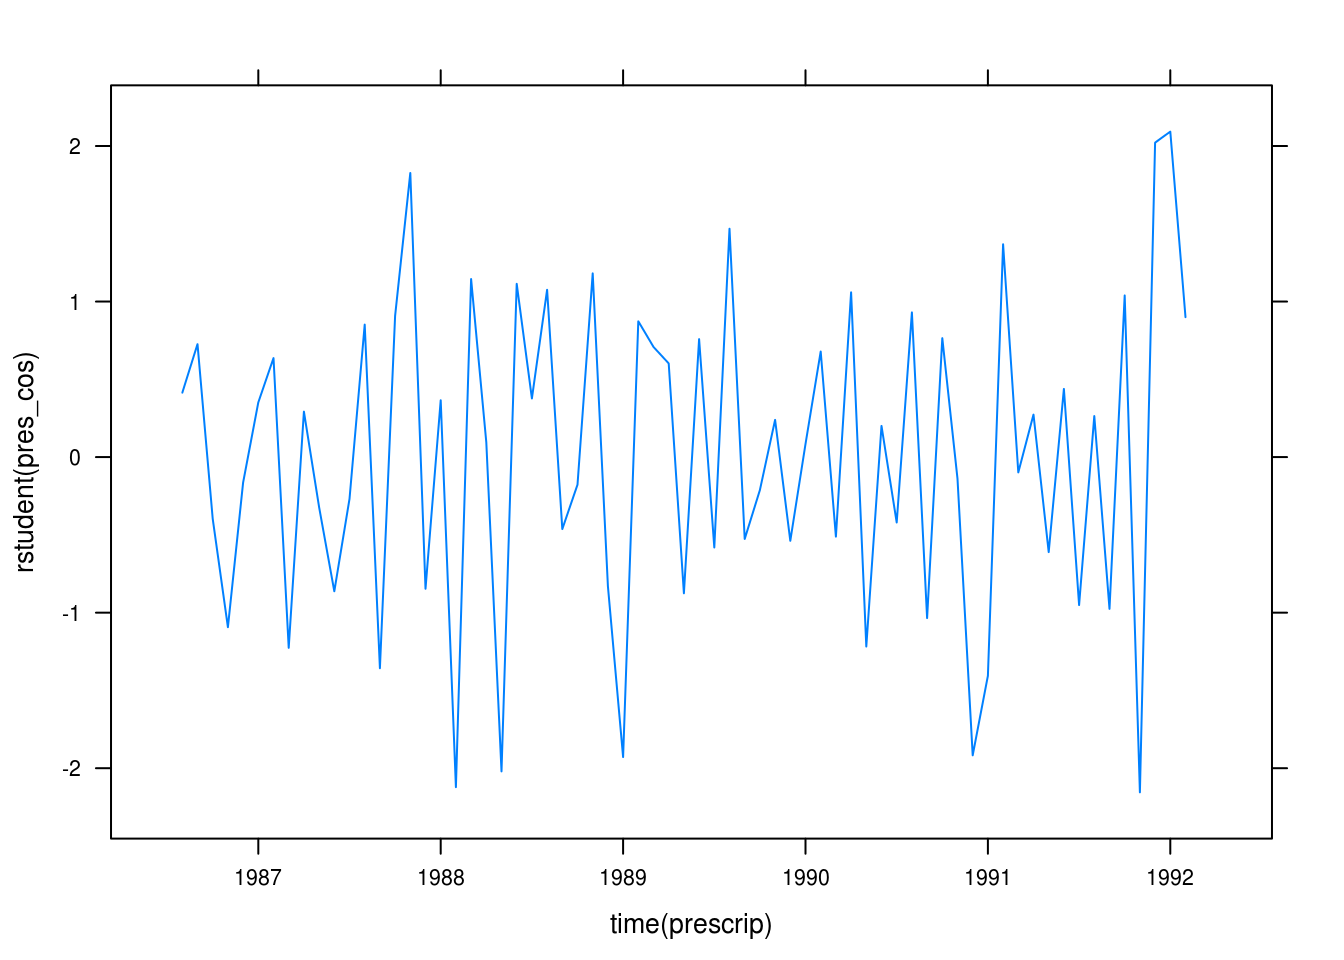
\includegraphics{TSAsolutions_files/figure-latex/cos-resid-1.pdf}
\caption{\label{fig:cos-resid}Residuals for our cosine model.}
\end{figure}

The residual plot in Figure \ref{cos-resid} looks rather random.

\end{document}
